\documentclass[aspectratio=169,10pt]{beamer}

\usepackage[T1]{fontenc}
\usepackage{array}
\usepackage{booktabs}
\usepackage{listings}
\usepackage{tabularx}
\usepackage{tikz}
\usepackage{xcolor}
\usetikzlibrary{arrows.meta,positioning,shapes.geometric}

\usetheme{Madrid}
\setbeamertemplate{navigation symbols}{}
\setbeamertemplate{caption}[numbered]

\definecolor{ieeeblue}{RGB}{0,70,130}
\definecolor{ieeelight}{RGB}{232,241,250}
\definecolor{stagegreen}{RGB}{0,122,90}
\definecolor{stageorange}{RGB}{190,105,20}
\definecolor{softgray}{RGB}{245,247,250}
\definecolor{codegray}{RGB}{65,65,65}

\setbeamercolor{palette primary}{bg=ieeeblue,fg=white}
\setbeamercolor{palette secondary}{bg=ieeeblue!85!black,fg=white}
\setbeamercolor{palette tertiary}{bg=ieeeblue!70!black,fg=white}
\setbeamercolor{frametitle}{bg=ieeeblue,fg=white}
\setbeamercolor{title}{fg=ieeeblue}
\setbeamercolor{block title}{bg=ieeeblue,fg=white}
\setbeamercolor{block body}{bg=ieeelight,fg=black}

\setbeamertemplate{footline}{
  \leavevmode
  \hbox{
    \begin{beamercolorbox}[wd=.34\paperwidth,ht=1.8ex,dp=.6ex,leftskip=1em]{author in head/foot}
      Siliconesignal Technologies
    \end{beamercolorbox}
    \begin{beamercolorbox}[wd=.46\paperwidth,ht=1.8ex,dp=.6ex,center]{title in head/foot}
      Gemmini ONNX-MLIR pipeline
    \end{beamercolorbox}
    \begin{beamercolorbox}[wd=.20\paperwidth,ht=1.8ex,dp=.6ex,rightskip=1em plus1fil]{date in head/foot}
      \insertframenumber{} / \inserttotalframenumber
    \end{beamercolorbox}
  }
  \hbox{
    \begin{beamercolorbox}[wd=\paperwidth,ht=1.9ex,dp=.6ex,center]{title in head/foot}
      {\fontsize{3.8}{4.3}\selectfont
      Paths:
      \href{run:/home/lahcen/toolchains/onnx-mlir-xcompile/onnx-mlir/src/Accelerators/Gemmini}{src/Accelerators/Gemmini/}
      \quad|\quad
      \href{run:/home/lahcen/toolchains/onnx-mlir-xcompile/onnx-mlir/gemmini/tests/15-resnet18-float}{gemmini/tests/15-resnet18-float/}}
    \end{beamercolorbox}
  }
}

\lstdefinestyle{cmdstyle}{
  basicstyle=\ttfamily\tiny\color{codegray},
  backgroundcolor=\color{softgray},
  frame=single,
  rulecolor=\color{ieeeblue!35},
  breaklines=true,
  columns=fullflexible,
  keepspaces=true,
  showstringspaces=false
}
\lstset{style=cmdstyle}

\newcommand{\code}[1]{\texttt{\footnotesize #1}}
\newcommand{\tinycode}[1]{\texttt{\tiny #1}}
\newcommand{\repoRoot}{/home/lahcen/toolchains/onnx-mlir-xcompile/onnx-mlir}
\newcommand{\pathcode}[1]{\href{run:\repoRoot/#1}{\texttt{\scriptsize #1}}}
\newcommand{\edgeword}[1]{\textcolor{red!75!black}{\textbf{#1}}}
\newcommand{\withoutit}[1]{\vspace{0.2em}{\tiny\color{codegray}\edgeword{Without it:} #1}}
\newcommand{\sectiondivider}[2]{
  \begin{frame}[plain]
    \vspace*{1.75cm}
    \begin{beamercolorbox}[wd=\paperwidth,ht=1.65cm,dp=0cm,center]{frametitle}
      \vbox to 1.65cm{\vfil{\Large\bfseries #1}\vfil}
    \end{beamercolorbox}
    \vspace{0.65cm}
    \begin{center}
      {\large #2}
    \end{center}
  \end{frame}
}

\title[Gemmini Backend Project]{Project: Gemmini Accelerator Backend for ONNX-MLIR}
\subtitle{Gemmini Pipeline in ONNX-MLIR: From ONNX Model to RISC-V Binary and Gemmini Execution}
\author{Siliconesignal Technologies}
\institute{}
\date{July 15, 2026}

\begin{document}

% 1
\begin{frame}[plain]
  \vspace*{1.95cm}
  \begin{beamercolorbox}[wd=\paperwidth,ht=2.15cm,dp=0cm,center]{frametitle}
    \vbox to 2.15cm{\vfil
      {\Large\bfseries Project: Gemmini Accelerator Backend for ONNX-MLIR}
    \vfil}
  \end{beamercolorbox}
  \vspace{0.65cm}
  \begin{center}
    {\large Gemmini Pipeline in ONNX-MLIR}\\[0.35cm]
    {\normalsize From ONNX Model to RISC-V Binary and Gemmini Execution}\\[0.9cm]
    {\large Siliconesignal Technologies}\\[0.25cm]
    {\normalsize July 15, 2026}\\[0.75cm]
    \pathcode{src/Accelerators/Gemmini/}
  \end{center}
\end{frame}

% 2
\sectiondivider{Big Picture}{Start with the whole path before diving into files, functions, and ABI details.}

% 2
\begin{frame}{How ONNX Moves to FPGA Execution}
  \centering
  \resizebox{0.98\textwidth}{!}{%
  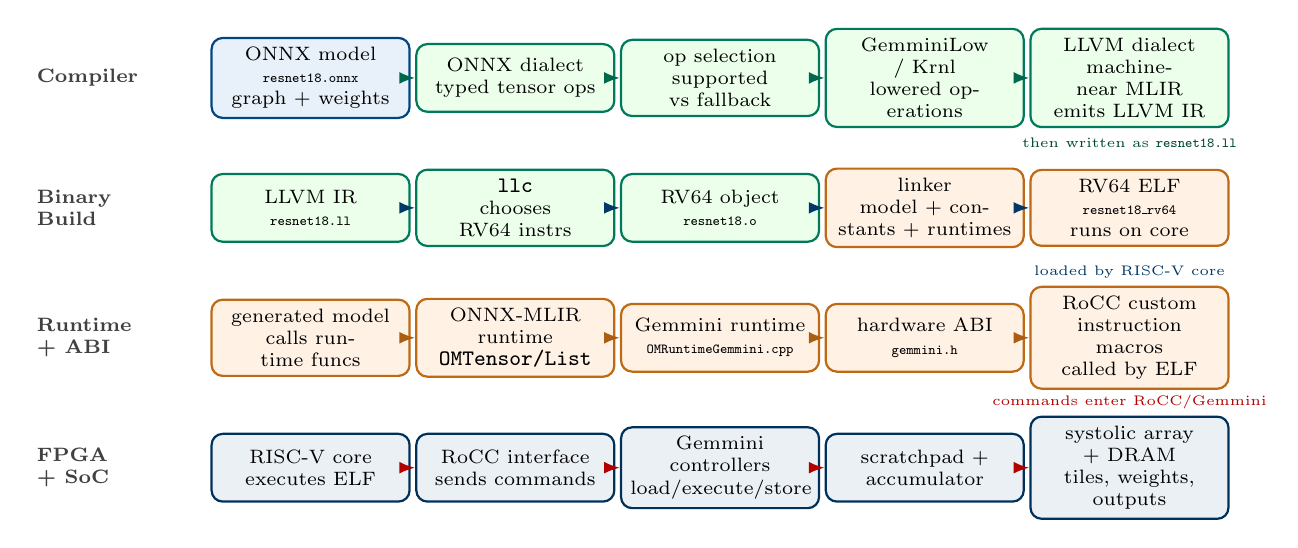
\begin{tikzpicture}[
    lane/.style={font=\scriptsize\bfseries\color{codegray},align=left,text width=1.55cm,anchor=west},
    src/.style={rectangle,rounded corners,draw=ieeeblue,fill=ieeelight,thick,
      text width=2.28cm,minimum height=0.86cm,align=center,font=\scriptsize},
    comp/.style={rectangle,rounded corners,draw=stagegreen,fill=green!8,thick,
      text width=2.28cm,minimum height=0.86cm,align=center,font=\scriptsize},
    rt/.style={rectangle,rounded corners,draw=stageorange,fill=orange!10,thick,
      text width=2.28cm,minimum height=0.86cm,align=center,font=\scriptsize},
    hw/.style={rectangle,rounded corners,draw=ieeeblue!70!black,fill=ieeeblue!8,thick,
      text width=2.28cm,minimum height=0.86cm,align=center,font=\scriptsize},
    compilearrow/.style={-{Latex[length=2mm]},thick,draw=stagegreen!85!black},
    buildarrow/.style={-{Latex[length=2mm]},thick,draw=ieeeblue!80!black},
    runtimearrow/.style={-{Latex[length=2mm]},thick,draw=stageorange!90!black},
    hwarrow/.style={-{Latex[length=2mm]},thick,draw=red!70!black},
    notelabel/.style={font=\tiny,fill=white,inner sep=1pt,text=black}
  ]
    \node[lane] at (-0.45,0) {Compiler};
    \node[src] (onnx) at (3.15,0) {ONNX model\\\tinycode{resnet18.onnx}\\graph + weights};
    \node[comp] (onnxmlir) at (5.75,0) {ONNX dialect\\typed tensor ops};
    \node[comp] (select) at (8.35,0) {op selection\\supported vs fallback};
    \node[comp] (gemlow) at (10.95,0) {GemminiLow / Krnl\\lowered operations};
    \node[comp] (llvmmlir) at (13.55,0) {LLVM dialect\\machine-near MLIR\\emits LLVM IR};

    \node[lane] at (-0.45,-1.65) {Binary\\Build};
    \node[comp] (llvmir) at (3.15,-1.65) {LLVM IR\\\tinycode{resnet18.ll}};
    \node[comp] (llc) at (5.75,-1.65) {\code{llc}\\chooses RV64 instrs};
    \node[comp] (obj) at (8.35,-1.65) {RV64 object\\\tinycode{resnet18.o}};
    \node[rt] (linker) at (10.95,-1.65) {linker\\model + constants + runtimes};
    \node[rt] (elf) at (13.55,-1.65) {RV64 ELF\\\tinycode{resnet18\_rv64}\\runs on core};

    \node[lane] at (-0.45,-3.30) {Runtime\\+ ABI};
    \node[rt] (modelcode) at (3.15,-3.30) {generated model\\calls runtime funcs};
    \node[rt] (onnxrt) at (5.75,-3.30) {ONNX-MLIR runtime\\\code{OMTensor/List}};
    \node[rt] (runtime) at (8.35,-3.30) {Gemmini runtime\\\tinycode{OMRuntimeGemmini.cpp}};
    \node[rt] (abi) at (10.95,-3.30) {hardware ABI\\\tinycode{gemmini.h}};
    \node[rt] (rocc) at (13.55,-3.30) {RoCC custom\\instruction macros\\called by ELF};

    \node[lane] at (-0.45,-4.95) {FPGA\\+ SoC};
    \node[hw] (core) at (3.15,-4.95) {RISC-V core\\executes ELF};
    \node[hw] (roccif) at (5.75,-4.95) {RoCC interface\\sends commands};
    \node[hw] (ctrl) at (8.35,-4.95) {Gemmini controllers\\load/execute/store};
    \node[hw] (spad) at (10.95,-4.95) {scratchpad +\\accumulator};
    \node[hw] (array) at (13.55,-4.95) {systolic array + DRAM\\tiles, weights, outputs};

    \draw[compilearrow] (onnx) -- (onnxmlir);
    \draw[compilearrow] (onnxmlir) -- (select);
    \draw[compilearrow] (select) -- (gemlow);
    \draw[compilearrow] (gemlow) -- (llvmmlir);

    \draw[buildarrow] (llvmir) -- (llc);
    \draw[buildarrow] (llc) -- (obj);
    \draw[buildarrow] (obj) -- (linker);
    \draw[buildarrow] (linker) -- (elf);

    \draw[runtimearrow] (modelcode) -- (onnxrt);
    \draw[runtimearrow] (onnxrt) -- (runtime);
    \draw[runtimearrow] (runtime) -- (abi);
    \draw[runtimearrow] (abi) -- (rocc);

    \draw[hwarrow] (core) -- (roccif);
    \draw[hwarrow] (roccif) -- (ctrl);
    \draw[hwarrow] (ctrl) -- (spad);
    \draw[hwarrow] (spad) -- (array);

    \node[notelabel,text=stagegreen!60!black] at (13.55,-0.82) {then written as \tinycode{resnet18.ll}};
    \node[notelabel,text=ieeeblue!80!black] at (13.55,-2.47) {loaded by RISC-V core};
    \node[notelabel,text=red!70!black] at (13.55,-4.12) {commands enter RoCC/Gemmini};
  \end{tikzpicture}
  }
  \vfill
  \begin{minipage}{0.94\textwidth}
    {\tiny\color{codegray}\textbf{How to Read This Slide:}
    green arrows = compiler lowering, blue arrows = binary build/link, orange arrows = runtime/ABI calls, red arrows = hardware command/data movement.
    Text boxes are separated by lanes to avoid mixing source files, compiler IR, runtime code, and FPGA blocks.}
  \end{minipage}
\end{frame}

% 2a
\begin{frame}{Pipeline Summary: Why Each Layer Exists}
  \scriptsize
  \begin{tabularx}{\textwidth}{@{}lXX@{}}
    \toprule
    Layer & Why it exists & What it produces \\
    \midrule
    \edgeword{Compiler IR} &
      Keeps model meaning visible while choosing Gemmini or fallback paths. &
      ONNX, Gemmini, GemminiLow, Krnl, and LLVM dialect forms. \\
    \edgeword{Binary build} &
      Turns typed LLVM IR into RV64 machine code and links required runtimes. &
      Object files, linked ELF, constants, runtime symbols. \\
    \edgeword{Runtime} &
      Gives generated model code stable functions that understand tensor descriptors. &
      Calls such as \code{om\_gemmini\_conv\_f32}. \\
    \edgeword{ABI} &
      Makes separately compiled code and hardware commands agree at binary level. &
      C calls, \code{gemmini.h} macros, RoCC instruction fields. \\
    \edgeword{Hardware} &
      Executes tiled matrix operations using scratchpad, accumulator, and systolic array. &
      Gemmini load, execute, and store behavior. \\
    \bottomrule
  \end{tabularx}
  \vspace{0.5em}
  \begin{block}{One sentence}
    The compiler decides and lowers; the runtime bridges tensors to helper code; the ABI keeps binary calls and hardware commands correct.
  \end{block}
\end{frame}

% 2b
\begin{frame}{Why ONNX-MLIR Is Useful}
  \scriptsize
  \begin{block}{Paper basis}
    Based on \textit{Compiling ONNX Neural Network Models Using MLIR} by Tian Jin, Gheorghe-Teodor Bercea, Tung D. Le, Tong Chen, Gong Su, Haruki Imai, Yasushi Negishi, Anh Leu, Kevin O'Brien, Kiyokuni Kawachiya, and Alexandre E. Eichenberger.
  \end{block}

  \vspace{0.3em}
  \centering
  \resizebox{0.96\textwidth}{!}{%
  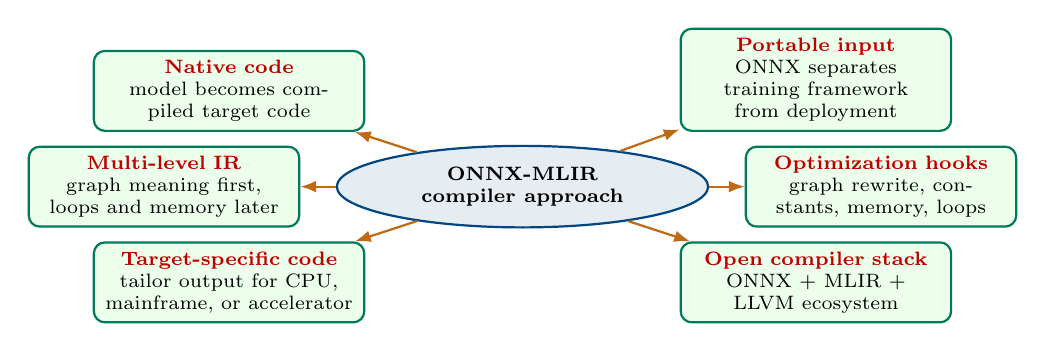
\begin{tikzpicture}[
    node distance=0.45cm,
    center/.style={ellipse,draw=ieeeblue,fill=ieeeblue!10,thick,
      text width=3.1cm,minimum height=1.0cm,align=center,font=\scriptsize\bfseries},
    benefit/.style={rectangle,rounded corners,draw=stagegreen,fill=green!8,thick,
      text width=3.2cm,minimum height=0.82cm,align=center,font=\scriptsize},
    arrow/.style={-{Latex[length=2mm]},thick,draw=stageorange}
  ]
    \node[center] (core) {ONNX-MLIR\\compiler approach};
    \node[benefit,above left=of core] (native) {\edgeword{Native code}\\model becomes compiled target code};
    \node[benefit,above right=of core] (portable) {\edgeword{Portable input}\\ONNX separates training framework from deployment};
    \node[benefit,left=of core] (multi) {\edgeword{Multi-level IR}\\graph meaning first, loops and memory later};
    \node[benefit,right=of core] (opt) {\edgeword{Optimization hooks}\\graph rewrite, constants, memory, loops};
    \node[benefit,below left=of core] (target) {\edgeword{Target-specific code}\\tailor output for CPU, mainframe, or accelerator};
    \node[benefit,below right=of core] (open) {\edgeword{Open compiler stack}\\ONNX + MLIR + LLVM ecosystem};

    \draw[arrow] (core) -- (native);
    \draw[arrow] (core) -- (portable);
    \draw[arrow] (core) -- (multi);
    \draw[arrow] (core) -- (opt);
    \draw[arrow] (core) -- (target);
    \draw[arrow] (core) -- (open);
  \end{tikzpicture}}

  \vspace{0.35em}
  {\tiny Source: \href{https://arxiv.org/abs/2008.08272}{arXiv:2008.08272, Compiling ONNX Neural Network Models Using MLIR}}
\end{frame}

% 2c
\begin{frame}{Why Compile Instead of Only Calling Libraries?}
  \scriptsize
  \begin{columns}[T,onlytextwidth]
    \begin{column}{0.48\textwidth}
      \begin{block}{Library-call approach}
        Replace model operations with calls into an optimized library.
      \end{block}
      \begin{tabularx}{\textwidth}{@{}lX@{}}
        \toprule
        Issue & Why it matters \\
        \midrule
        \edgeword{Coverage limit} & Only operations with available library functions are easy to rewrite. \\
        \edgeword{Extra packages} & Deployment may depend on target-specific runtime stacks. \\
        \edgeword{Generic kernels} & One library function may not fit every model shape or memory pattern. \\
        \bottomrule
      \end{tabularx}
    \end{column}
    \begin{column}{0.48\textwidth}
      \begin{block}{ONNX-MLIR compiler approach}
        Rewrite the trained model into native code for the target.
      \end{block}
      \begin{tabularx}{\textwidth}{@{}lX@{}}
        \toprule
        Benefit & Why it matters \\
        \midrule
        \edgeword{Specialization} & The compiler can tailor loops, memory, and calls for this exact model. \\
        \edgeword{Optimization} & Graph rewriting, constant propagation, memory planning, and loop transforms can happen before runtime. \\
        \edgeword{Deployment} & The final artifact can be a library or executable with less runtime decision making. \\
        \bottomrule
      \end{tabularx}
    \end{column}
  \end{columns}

  \vspace{0.45em}
  \begin{block}{Connection to Gemmini}
    Gemmini uses the same compiler logic, but adds accelerator-specific dialects, passes, runtime calls, and ABI instructions after ONNX-MLIR has preserved the model semantics.
  \end{block}
\end{frame}

% 2d
\begin{frame}{ONNX-MLIR Benefits Come from Multiple IR Levels}
  \centering
  \resizebox{0.96\textwidth}{!}{%
  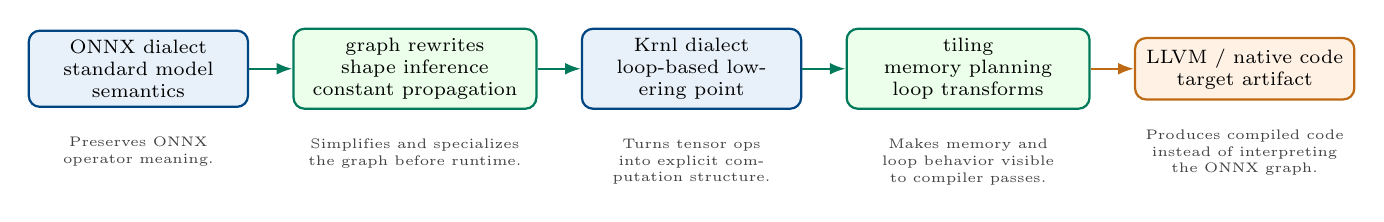
\begin{tikzpicture}[
    node distance=0.55cm,
    ir/.style={rectangle,rounded corners,draw=ieeeblue,fill=ieeelight,thick,
      text width=2.55cm,minimum height=0.78cm,align=center,font=\scriptsize},
    pass/.style={rectangle,rounded corners,draw=stagegreen,fill=green!8,thick,
      text width=2.85cm,minimum height=0.78cm,align=center,font=\scriptsize},
    artifactbox/.style={rectangle,rounded corners,draw=stageorange,fill=orange!10,thick,
      text width=2.55cm,minimum height=0.78cm,align=center,font=\scriptsize},
    arrow/.style={-{Latex[length=2mm]},thick}
  ]
    \node[ir] (onnx) {ONNX dialect\\standard model semantics};
    \node[pass,right=of onnx] (graph) {graph rewrites\\shape inference\\constant propagation};
    \node[ir,right=of graph] (krnl) {Krnl dialect\\loop-based lowering point};
    \node[pass,right=of krnl] (loop) {tiling\\memory planning\\loop transforms};
    \node[artifactbox,right=of loop] (llvm) {LLVM / native code\\target artifact};

    \draw[arrow,draw=stagegreen] (onnx) -- (graph);
    \draw[arrow,draw=stagegreen] (graph) -- (krnl);
    \draw[arrow,draw=stagegreen] (krnl) -- (loop);
    \draw[arrow,draw=stageorange] (loop) -- (llvm);

    \node[font=\tiny,text=codegray,align=center,text width=2.55cm,below=0.25cm of onnx]
      {Preserves ONNX operator meaning.};
    \node[font=\tiny,text=codegray,align=center,text width=2.85cm,below=0.25cm of graph]
      {Simplifies and specializes the graph before runtime.};
    \node[font=\tiny,text=codegray,align=center,text width=2.55cm,below=0.25cm of krnl]
      {Turns tensor ops into explicit computation structure.};
    \node[font=\tiny,text=codegray,align=center,text width=2.85cm,below=0.25cm of loop]
      {Makes memory and loop behavior visible to compiler passes.};
    \node[font=\tiny,text=codegray,align=center,text width=2.55cm,below=0.25cm of llvm]
      {Produces compiled code instead of interpreting the ONNX graph.};
  \end{tikzpicture}}

  \vspace{0.55em}
  \scriptsize
  \begin{block}{Why this matters}
    Each IR level exposes a different kind of optimization: ONNX exposes graph semantics, Krnl exposes loops and memory, and LLVM exposes machine-code generation. Gemmini extends this idea with Gemmini and GemminiLow dialects for accelerator-aware lowering.
  \end{block}
\end{frame}

% 2e
\begin{frame}{Optimization Map from the ONNX-MLIR Paper}
  \centering
  \resizebox{0.97\textwidth}{!}{%
  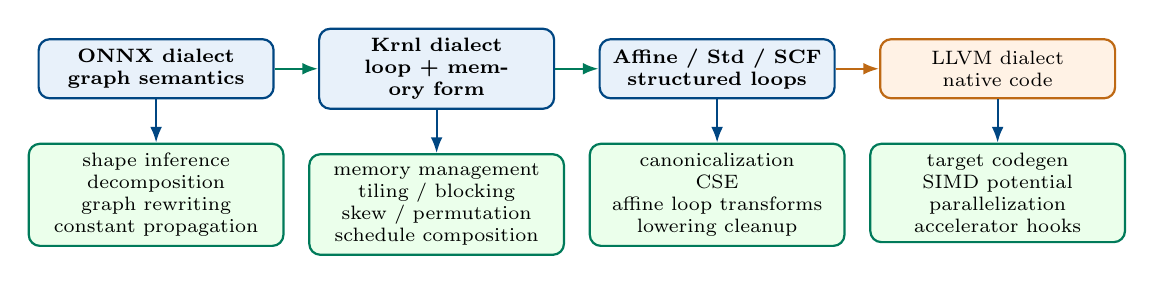
\begin{tikzpicture}[
    node distance=0.55cm,
    level/.style={rectangle,rounded corners,draw=ieeeblue,fill=ieeelight,thick,
      text width=2.75cm,minimum height=0.75cm,align=center,font=\scriptsize\bfseries},
    optbox/.style={rectangle,rounded corners,draw=stagegreen,fill=green!8,thick,
      text width=3.0cm,minimum height=0.75cm,align=center,font=\scriptsize},
    outbox/.style={rectangle,rounded corners,draw=stageorange,fill=orange!10,thick,
      text width=2.75cm,minimum height=0.75cm,align=center,font=\scriptsize},
    arrow/.style={-{Latex[length=2mm]},thick}
  ]
    \node[level] (onnx) {ONNX dialect\\graph semantics};
    \node[optbox,below=of onnx] (gopt) {shape inference\\decomposition\\graph rewriting\\constant propagation};
    \node[level,right=of onnx] (krnl) {Krnl dialect\\loop + memory form};
    \node[optbox,below=of krnl] (kopt) {memory management\\tiling / blocking\\skew / permutation\\schedule composition};
    \node[level,right=of krnl] (affine) {Affine / Std / SCF\\structured loops};
    \node[optbox,below=of affine] (aopt) {canonicalization\\CSE\\affine loop transforms\\lowering cleanup};
    \node[outbox,right=of affine] (llvm) {LLVM dialect\\native code};
    \node[optbox,below=of llvm] (native) {target codegen\\SIMD potential\\parallelization\\accelerator hooks};

    \draw[arrow,draw=stagegreen] (onnx) -- (krnl);
    \draw[arrow,draw=stagegreen] (krnl) -- (affine);
    \draw[arrow,draw=stageorange] (affine) -- (llvm);
    \draw[arrow,draw=ieeeblue] (onnx) -- (gopt);
    \draw[arrow,draw=ieeeblue] (krnl) -- (kopt);
    \draw[arrow,draw=ieeeblue] (affine) -- (aopt);
    \draw[arrow,draw=ieeeblue] (llvm) -- (native);
  \end{tikzpicture}}

  \vspace{0.45em}
  \scriptsize
  \begin{block}{Main idea}
    The paper's key benefit is not one single optimization. It is that each lowering level exposes a different optimization surface: graph transformations at ONNX level, loop and memory transformations at Krnl/Affine level, and native-code generation at LLVM level.
  \end{block}
\end{frame}

% 2f
\begin{frame}{Graph-Level Optimizations: Simplify the Model Early}
  \scriptsize
  \begin{tabularx}{\textwidth}{@{}lXX@{}}
    \toprule
    Optimization & What it does & Why it helps \\
    \midrule
    \edgeword{Operation decomposition} &
      Replaces complex ONNX ops with simpler supported ops. Example from the paper: \code{ReduceL1(x)} can become \code{ReduceSum(Abs(x))}. &
      The compiler only needs strong lowerings for a smaller core set of operations. Unsupported-looking models become easier to compile. \\
    \edgeword{Graph rewriting} &
      Replaces patterns of operations with better patterns. Example from the paper: \code{MatMul + Add} can become \code{Gemm}. &
      Removes redundant graph structure and exposes kernels that are easier to optimize or accelerate. \\
    \edgeword{Identity elimination} &
      Removes operations that only forward their input. &
      Reduces graph size and avoids generating useless runtime work. \\
    \bottomrule
  \end{tabularx}

  \vspace{0.45em}
  \centering
  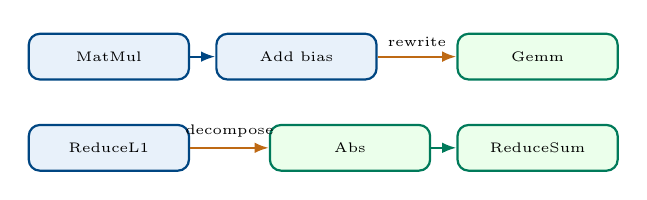
\begin{tikzpicture}[
    node distance=0.32cm,
    box/.style={rectangle,rounded corners,draw=ieeeblue,fill=ieeelight,thick,
      text width=1.8cm,minimum height=0.58cm,align=center,font=\tiny},
    good/.style={rectangle,rounded corners,draw=stagegreen,fill=green!8,thick,
      text width=1.8cm,minimum height=0.58cm,align=center,font=\tiny},
    arrow/.style={-{Latex[length=1.8mm]},thick}
  ]
    \node[box] (matmul) {MatMul};
    \node[box,right=of matmul] (add) {Add bias};
    \node[good,right=1.0cm of add] (gemm) {Gemm};
    \draw[arrow,draw=ieeeblue] (matmul) -- (add);
    \draw[arrow,draw=stageorange] (add) -- node[above,font=\tiny] {rewrite} (gemm);

    \node[box,below=0.55cm of matmul] (reduce) {ReduceL1};
    \node[good,right=1.0cm of reduce] (abs) {Abs};
    \node[good,right=of abs] (sum) {ReduceSum};
    \draw[arrow,draw=stageorange] (reduce) -- node[above,font=\tiny] {decompose} (abs);
    \draw[arrow,draw=stagegreen] (abs) -- (sum);
  \end{tikzpicture}
\end{frame}

% 2g
\begin{frame}{Shape, Constant, and Memory Optimizations}
  \scriptsize
  \begin{columns}[T,onlytextwidth]
    \begin{column}{0.32\textwidth}
      \begin{block}{\edgeword{Shape inference}}
        Infers ranked tensor shapes from ONNX operations and propagates them to consumers.
      \end{block}
      \withoutit{later passes see unknown tensor ranks, so buffer allocation and loop bounds become harder or impossible.}
    \end{column}
    \begin{column}{0.32\textwidth}
      \begin{block}{\edgeword{Constant propagation}}
        Computes operations at compile time when their inputs are constants, and normalizes expressions so more constants can fold.
      \end{block}
      \withoutit{weights, bias transforms, and static shape calculations may become unnecessary runtime work.}
    \end{column}
    \begin{column}{0.32\textwidth}
      \begin{block}{\edgeword{Memory management}}
        Converts abstract tensors into allocated buffers, tracks lifetimes, and prepares data for lower-level loops and calls.
      \end{block}
      \withoutit{compiled code would know the math but not where intermediate tensors should live.}
    \end{column}
  \end{columns}

  \vspace{0.45em}
  \centering
  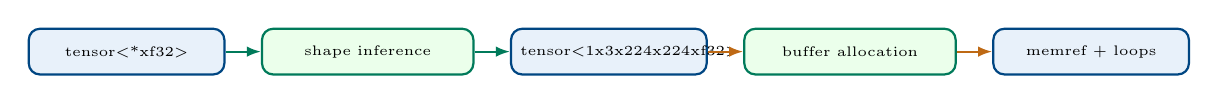
\begin{tikzpicture}[
    node distance=0.45cm,
    box/.style={rectangle,rounded corners,draw=ieeeblue,fill=ieeelight,thick,
      text width=2.25cm,minimum height=0.58cm,align=center,font=\tiny},
    optbox/.style={rectangle,rounded corners,draw=stagegreen,fill=green!8,thick,
      text width=2.45cm,minimum height=0.58cm,align=center,font=\tiny},
    arrow/.style={-{Latex[length=1.8mm]},thick}
  ]
    \node[box] (unknown) {tensor<*xf32>};
    \node[optbox,right=of unknown] (shape) {shape inference};
    \node[box,right=of shape] (ranked) {tensor<1x3x224x224xf32>};
    \node[optbox,right=of ranked] (alloc) {buffer allocation};
    \node[box,right=of alloc] (memref) {memref + loops};
    \draw[arrow,draw=stagegreen] (unknown) -- (shape);
    \draw[arrow,draw=stagegreen] (shape) -- (ranked);
    \draw[arrow,draw=stageorange] (ranked) -- (alloc);
    \draw[arrow,draw=stageorange] (alloc) -- (memref);
  \end{tikzpicture}
\end{frame}

% 2h
\begin{frame}[fragile]{Krnl Optimizations: Separate What to Compute from How to Schedule}
  \scriptsize
  \begin{block}{Krnl purpose from the paper}
    Krnl is a loop-based dialect that gives all ONNX operations a common lowering point. It keeps program semantics separate from schedules, so the compiler can change loop order, tile size, or blocking strategy without changing the mathematical meaning.
  \end{block}

  \vspace{0.3em}
  \begin{columns}[T,onlytextwidth]
    \begin{column}{0.47\textwidth}
\begin{lstlisting}
%ii = krnl.define_loops 1
krnl.iterate(%ii) with (%ii -> %i = 0 to 10) {
  // original computation
}
\end{lstlisting}
      \centering{\tiny Original loop: simple semantics.}
    \end{column}
    \begin{column}{0.47\textwidth}
\begin{lstlisting}
%ii = krnl.define_loops 1
%ib, %il = krnl.block %ii 2
krnl.iterate(%ib, %il) with (%ii -> %i = 0 to 10) {
  // same computation, scheduled in tiles
}
\end{lstlisting}
      \centering{\tiny Scheduled loop: same math, different execution plan.}
    \end{column}
  \end{columns}

  \vspace{0.4em}
  \begin{tabularx}{\textwidth}{@{}lX@{}}
    \toprule
    Schedule optimization & Meaning \\
    \midrule
    \edgeword{Blocking / tiling} & Split a loop into outer and inner loops so data can fit cache, scratchpad, or accelerator tiles. \\
    \edgeword{Permutation} & Reorder loops to improve memory access order or match hardware traversal. \\
    \edgeword{Skewing} & Change loop coordinates to expose parallelism or legalize transformations. \\
    \edgeword{Composition} & Combine schedules, such as tile then permute, while keeping the original computation readable. \\
    \bottomrule
  \end{tabularx}
\end{frame}

% 2i
\begin{frame}{How These Optimizations Help the Gemmini Backend}
  \scriptsize
  \begin{tabularx}{\textwidth}{@{}lXX@{}}
    \toprule
    ONNX-MLIR optimization idea & General benefit & Gemmini-specific benefit \\
    \midrule
    \edgeword{Shape inference} &
      Makes tensor ranks and dimensions explicit. &
      Gives Conv/MatMul lowering concrete dimensions for tile sizes, scratchpad planning, and runtime parameters. \\
    \edgeword{Graph rewriting} &
      Turns model patterns into better compiler patterns. &
      Helps identify accelerator-friendly operations such as Conv, MatMul, Gemm-like forms, Add, Pool, and Relu. \\
    \edgeword{Constant propagation} &
      Moves static computation to compile time. &
      Keeps weights and derived constants in the binary instead of recomputing them during inference. \\
    \edgeword{Memory management} &
      Decides where intermediate tensors live. &
      Bridges normal memory buffers to Gemmini runtime calls that move data into scratchpad and accumulator storage. \\
    \edgeword{Loop tiling} &
      Breaks large tensor work into smaller chunks. &
      Matches Gemmini's tile-based systolic array execution and local memory capacity. \\
    \bottomrule
  \end{tabularx}

  \vspace{0.45em}
  \begin{block}{Key message}
    ONNX-MLIR optimizations are not only CPU optimizations. They are also preparation steps that make accelerator lowering possible: operations become legal, shapes become known, constants become stable, memory becomes explicit, and loops become tileable.
  \end{block}
\end{frame}

% 2j
\begin{frame}{Optimization Terms to Remember}
  \scriptsize
  \begin{tabularx}{\textwidth}{@{}lX@{}}
    \toprule
    Term & Simple definition \\
    \midrule
    \edgeword{Canonicalization} & Rewrite IR into a simpler standard form so later passes see fewer special cases. \\
    \edgeword{CSE} & Common subexpression elimination: if the same computation appears twice, compute it once and reuse it. \\
    \edgeword{DRR} & Declarative Rewrite Rule: TableGen-based pattern that says ``replace this operation graph with that one.'' \\
    \edgeword{Polyhedral optimization} & Mathematical loop optimization for regular loop nests; useful for tiling, scheduling, and memory locality. \\
    \edgeword{Loop fusion} & Combine neighboring loops so data loaded once can be reused before it leaves cache or scratchpad. \\
    \edgeword{SIMD optimization} & Generate vector instructions so one CPU instruction operates on multiple data elements. \\
    \edgeword{Parallelization} & Split independent work across cores, threads, lanes, or accelerator units. \\
    \bottomrule
  \end{tabularx}

  \vspace{0.45em}
  {\tiny Source basis: \href{https://arxiv.org/abs/2008.08272}{Compiling ONNX Neural Network Models Using MLIR}; terms are explained here in presentation language and connected to the Gemmini backend.}
\end{frame}

% 2k
\begin{frame}{Who Uses ONNX-MLIR and Why It Matters}
  \scriptsize
  \begin{block}{Context}
    ONNX-MLIR is not end-user software. It is a developer-facing compiler framework, so adoption is concentrated around hardware vendors, cloud/runtime builders, AI framework teams, and compiler researchers.
  \end{block}

  \vspace{0.25em}
  \begin{tabularx}{\textwidth}{@{}lXX@{}}
    \toprule
    Group & Role in the ecosystem & Why it matters for this project \\
    \midrule
    \edgeword{IBM} &
      Origin and named adopter. The ONNX-MLIR README lists IBM zDLC using ONNX-MLIR technology for IBM Telum servers. &
      Shows the same compiler idea can target real accelerator-backed production hardware. \\
    \edgeword{Microsoft + Meta} &
      Core ONNX ecosystem leaders and ONNX standard originators; relevant to model interchange and framework compatibility. &
      ONNX-MLIR depends on stable ONNX semantics before any Gemmini lowering can happen. \\
    \edgeword{Arm / edge CPU ecosystem} &
      Important target space for efficient neural-network lowering on CPUs and edge processors. &
      Reinforces why compiler IR, lowering, and hardware-aware code generation matter beyond one chip. \\
    \edgeword{Serving + downstream hardware} &
      Related serving projects and custom accelerator forks can use ONNX-MLIR as a pluggable frontend. &
      Gemmini follows this pattern: reuse ONNX-MLIR frontend/compiler structure, then add accelerator-specific dialect/runtime/ABI. \\
    \bottomrule
  \end{tabularx}

  \vspace{0.35em}
  {\tiny Sources:
  \href{https://github.com/onnx/onnx-mlir}{ONNX-MLIR GitHub README}
  \quad|\quad
  \href{https://www.youtube.com/watch?v=V70XXsPVrzg}{ONNX-MLIR ecosystem talk}
  \quad|\quad
  \href{https://www.youtube.com/watch?v=cXHTu2wI5Ps}{IBM Research talk}
  \quad|\quad
  \href{https://www.youtube.com/watch?v=kJ9JoOoOj1A}{Arm/compiler talk}}
\end{frame}

% 3
\begin{frame}{Why This Project Exists}
  \begin{block}{Goal}
    Compile neural-network models represented in ONNX into RISC-V executables that can use the Gemmini matrix accelerator.
  \end{block}
  \begin{itemize}
    \item ONNX expresses the model as graph operations such as Conv, MatMul, Add, Relu, and Pool.
    \item ONNX-MLIR translates the graph through progressively lower compiler IR levels.
    \item Gemmini-specific passes identify operations that should run on the accelerator.
    \item The final binary contains normal RISC-V code plus runtime calls and Gemmini custom instructions.
  \end{itemize}
\end{frame}

% 4
\begin{frame}{How the Final Binary Is Built}
  \centering
  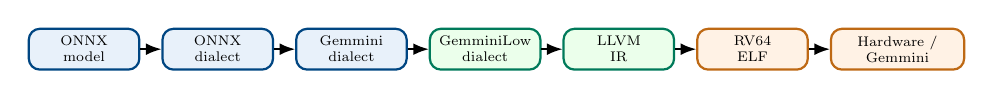
\begin{tikzpicture}[
    scale=0.72,
    every node/.style={transform shape},
    node distance=0.38cm,
    box/.style={rectangle,rounded corners,draw=ieeeblue,fill=ieeelight,thick,
      minimum width=1.95cm,minimum height=0.72cm,align=center,font=\scriptsize},
    low/.style={rectangle,rounded corners,draw=stagegreen,fill=green!8,thick,
      minimum width=1.95cm,minimum height=0.72cm,align=center,font=\scriptsize},
    hw/.style={rectangle,rounded corners,draw=stageorange,fill=orange!10,thick,
      minimum width=1.95cm,minimum height=0.72cm,align=center,font=\scriptsize},
    arrow/.style={-{Latex[length=2mm]},thick}
  ]
    \node[box] (onnx) {ONNX\\model};
    \node[box,right=of onnx] (onnxd) {ONNX\\dialect};
    \node[box,right=of onnxd] (gemmini) {Gemmini\\dialect};
    \node[low,right=of gemmini] (low) {GemminiLow\\dialect};
    \node[low,right=of low] (llvm) {LLVM\\IR};
    \node[hw,right=of llvm] (elf) {RV64\\ELF};
    \node[hw,minimum width=2.35cm,right=of elf] (hw) {Hardware /\\Gemmini};
    \draw[arrow] (onnx) -- (onnxd);
    \draw[arrow] (onnxd) -- (gemmini);
    \draw[arrow] (gemmini) -- (low);
    \draw[arrow] (low) -- (llvm);
    \draw[arrow] (llvm) -- (elf);
    \draw[arrow] (elf) -- (hw);
  \end{tikzpicture}
  \vspace{0.7em}
  \begin{block}{Important}
    The final RV64 executable is a linked program, not a one-to-one copy of the ONNX graph.
    It contains:
    \begin{itemize}
      \item generated model code for graph control, tensor setup, and calls;
      \item constants such as weights and bias tensors in read-only data;
      \item ONNX-MLIR runtime code for \code{OMTensor} and \code{OMTensorList};
      \item Gemmini runtime code such as \code{om\_gemmini\_conv\_f32};
      \item Gemmini hardware ABI calls that become RISC-V custom instructions.
    \end{itemize}
  \end{block}
  \vspace{-0.2em}
  Each step removes abstraction: graph operation, compiler operation, runtime call, object symbol, linked address, and finally disassembled RISC-V instructions.
\end{frame}

% 5
\sectiondivider{Core Terms}{Define the vocabulary before using it repeatedly in compiler and runtime diagrams.}

% 5
\begin{frame}{ABI Defines the Binary Contract}
  \begin{columns}
    \begin{column}{0.45\textwidth}
      \centering
      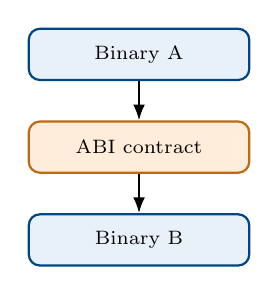
\begin{tikzpicture}[node distance=0.5cm, every node/.style={transform shape},
        box/.style={rectangle,rounded corners,draw=ieeeblue,fill=ieeelight,thick,
          minimum width=2.8cm,minimum height=0.65cm,align=center,font=\scriptsize},
        abi/.style={rectangle,rounded corners,draw=stageorange,fill=orange!15,thick,
          minimum width=2.8cm,minimum height=0.65cm,align=center,font=\scriptsize},
        arrow/.style={-{Latex[length=2mm]},thick}]
        \node[box] (a) {Binary A};
        \node[abi,below=of a] (b) {ABI contract};
        \node[box,below=of b] (c) {Binary B};
        \draw[arrow] (a) -- (b);
        \draw[arrow] (b) -- (c);
      \end{tikzpicture}
    \end{column}
    \begin{column}{0.52\textwidth}
      \begin{block}{Application Binary Interface}
        Rules that let compiled code and binary components call each other correctly.
      \end{block}
      \begin{itemize}
        \item Calling convention, registers, stack.
        \item Pointer sizes, alignment, data layout.
        \item Symbol names, relocation records, libraries.
        \item Linux example: ELF binary + libc + syscalls.
        \item Gemmini example: runtime calls + hardware commands.
      \end{itemize}
    \end{column}
  \end{columns}
\end{frame}

% 5b
\begin{frame}{How Linux Uses an ABI}
  \centering
  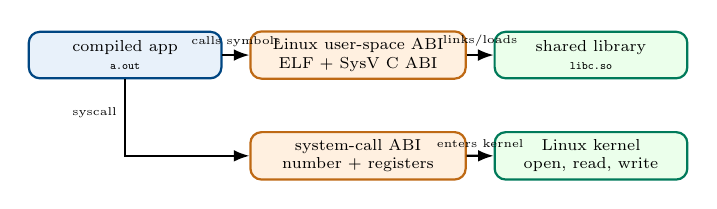
\begin{tikzpicture}[
    scale=0.82,
    every node/.style={transform shape},
    node distance=0.42cm,
    bin/.style={rectangle,rounded corners,draw=ieeeblue,fill=ieeelight,thick,
      text width=2.75cm,minimum height=0.72cm,align=center,font=\scriptsize},
    abi/.style={rectangle,rounded corners,draw=stageorange,fill=orange!12,thick,
      text width=3.1cm,minimum height=0.72cm,align=center,font=\scriptsize},
    sys/.style={rectangle,rounded corners,draw=stagegreen,fill=green!8,thick,
      text width=2.75cm,minimum height=0.72cm,align=center,font=\scriptsize},
    arrow/.style={-{Latex[length=2mm]},thick}
  ]
    \node[bin] (app) {compiled app\\\tinycode{a.out}};
    \node[abi,right=of app] (cabi) {Linux user-space ABI\\ELF + SysV C ABI};
    \node[sys,right=of cabi] (libc) {shared library\\\tinycode{libc.so}};
    \node[abi,below=0.8cm of cabi] (syscall) {system-call ABI\\number + registers};
    \node[sys,right=of syscall] (kernel) {Linux kernel\\open, read, write};

    \draw[arrow] (app) -- node[above,font=\tiny] {calls symbols} (cabi);
    \draw[arrow] (cabi) -- node[above,font=\tiny] {links/loads} (libc);
    \draw[arrow] (app) |- node[pos=0.22,left,font=\tiny] {syscall} (syscall);
    \draw[arrow] (syscall) -- node[above,font=\tiny] {enters kernel} (kernel);
  \end{tikzpicture}

  \vspace{0.4em}
  \begin{block}{Concrete Linux Meaning}
    A Linux binary works because it follows agreed binary rules: ELF file format, symbol names, register usage for function calls, stack layout, syscall numbers, and which registers carry syscall arguments.
  \end{block}
\end{frame}

% 5c
\begin{frame}{What Breaks Without an ABI?}
  \centering
  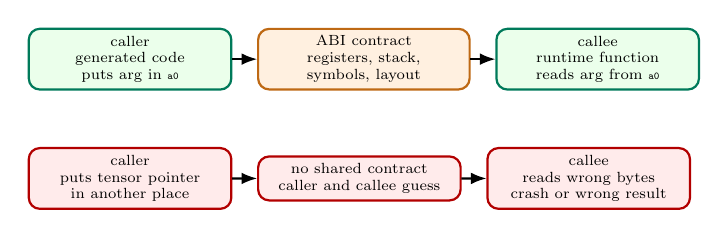
\begin{tikzpicture}[
    scale=0.76,
    every node/.style={transform shape},
    node distance=0.42cm,
    good/.style={rectangle,rounded corners,draw=stagegreen,fill=green!8,thick,
      text width=3.15cm,minimum height=0.72cm,align=center,font=\scriptsize},
    bad/.style={rectangle,rounded corners,draw=red!70!black,fill=red!8,thick,
      text width=3.15cm,minimum height=0.72cm,align=center,font=\scriptsize},
    abi/.style={rectangle,rounded corners,draw=stageorange,fill=orange!12,thick,
      text width=3.3cm,minimum height=0.72cm,align=center,font=\scriptsize},
    arrow/.style={-{Latex[length=2mm]},thick}
  ]
    \node[good] (caller) {caller\\generated code\\puts arg in \tinycode{a0}};
    \node[abi,right=of caller] (contract) {ABI contract\\registers, stack, symbols, layout};
    \node[good,right=of contract] (callee) {callee\\runtime function\\reads arg from \tinycode{a0}};
    \node[bad,below=0.95cm of caller] (wrongCaller) {caller\\puts tensor pointer\\in another place};
    \node[bad,right=of wrongCaller] (missing) {no shared contract\\caller and callee guess};
    \node[bad,right=of missing] (wrongCallee) {callee\\reads wrong bytes\\crash or wrong result};

    \draw[arrow] (caller) -- (contract);
    \draw[arrow] (contract) -- (callee);
    \draw[arrow] (wrongCaller) -- (missing);
    \draw[arrow] (missing) -- (wrongCallee);
  \end{tikzpicture}

  \vspace{0.35em}
  \begin{itemize}
    \item The caller is the code that starts the call; in this project it can be generated model code.
    \item The callee is the code receiving the call; here it can be \code{om\_gemmini\_conv\_f32}.
    \item Without an ABI, both sides may disagree on symbol names, registers, stack slots, and struct layout.
    \item The program may still link or run, but it can pass corrupted arguments to the runtime or hardware.
  \end{itemize}
\end{frame}

\begin{frame}{How Caller/Callee Mismatch Breaks Execution}
  \centering
  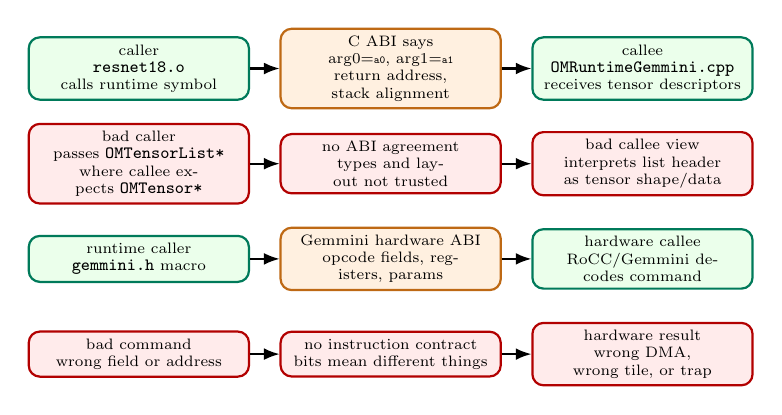
\begin{tikzpicture}[
    scale=0.78,
    every node/.style={transform shape},
    good/.style={rectangle,rounded corners,draw=stagegreen,fill=green!8,thick,
      text width=3.35cm,minimum height=0.72cm,align=center,font=\scriptsize},
    bad/.style={rectangle,rounded corners,draw=red!70!black,fill=red!8,thick,
      text width=3.35cm,minimum height=0.72cm,align=center,font=\scriptsize},
    abi/.style={rectangle,rounded corners,draw=stageorange,fill=orange!12,thick,
      text width=3.35cm,minimum height=0.72cm,align=center,font=\scriptsize},
    arrow/.style={-{Latex[length=2mm]},thick}
  ]
    \node[good] (model) at (0,0) {caller\\\code{resnet18.o}\\calls runtime symbol};
    \node[abi] (cabi) at (4.1,0) {C ABI says\\arg0=\tinycode{a0}, arg1=\tinycode{a1}\\return address, stack alignment};
    \node[good] (rt) at (8.2,0) {callee\\\code{OMRuntimeGemmini.cpp}\\receives tensor descriptors};

    \node[bad] (badmodel) at (0,-1.55) {bad caller\\passes \code{OMTensorList*}\\where callee expects \code{OMTensor*}};
    \node[bad] (badcontract) at (4.1,-1.55) {no ABI agreement\\types and layout not trusted};
    \node[bad] (badrt) at (8.2,-1.55) {bad callee view\\interprets list header\\as tensor shape/data};

    \node[good] (runtime) at (0,-3.1) {runtime caller\\\code{gemmini.h} macro};
    \node[abi] (hwabi) at (4.1,-3.1) {Gemmini hardware ABI\\opcode fields, registers, params};
    \node[good] (hw) at (8.2,-3.1) {hardware callee\\RoCC/Gemmini decodes command};

    \node[bad] (badcmd) at (0,-4.65) {bad command\\wrong field or address};
    \node[bad] (badhwabi) at (4.1,-4.65) {no instruction contract\\bits mean different things};
    \node[bad] (badhw) at (8.2,-4.65) {hardware result\\wrong DMA, wrong tile, or trap};

    \draw[arrow] (model) -- (cabi);
    \draw[arrow] (cabi) -- (rt);
    \draw[arrow] (badmodel) -- (badcontract);
    \draw[arrow] (badcontract) -- (badrt);
    \draw[arrow] (runtime) -- (hwabi);
    \draw[arrow] (hwabi) -- (hw);
    \draw[arrow] (badcmd) -- (badhwabi);
    \draw[arrow] (badhwabi) -- (badhw);
  \end{tikzpicture}

  \vspace{0.25em}
  \begin{minipage}{0.94\textwidth}
    {\tiny\color{codegray}
    \edgeword{Caller}: the side that starts a call or sends a command, for example \code{resnet18.o} or a \code{gemmini.h} macro.
    \edgeword{Callee}: the side that receives it, for example \code{OMRuntimeGemmini.cpp} or Gemmini hardware.
    The ABI is the shared promise that lets both sides understand the same call, data layout, and hardware command bits.}
  \end{minipage}
\end{frame}

% 5d
\begin{frame}{Where ABI Boundaries Appear in This Project}
  \centering
  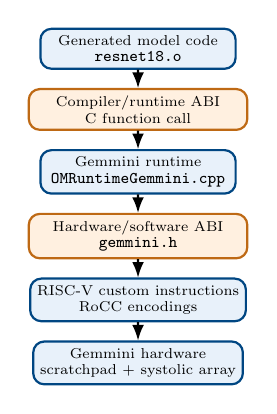
\begin{tikzpicture}[
    scale=0.74,
    every node/.style={transform shape},
    node distance=0.32cm,
    layer/.style={rectangle,rounded corners,draw=ieeeblue,fill=ieeelight,thick,
      minimum width=3.35cm,minimum height=0.62cm,align=center,font=\scriptsize},
    abi/.style={rectangle,rounded corners,draw=stageorange,fill=orange!12,thick,
      minimum width=3.75cm,minimum height=0.62cm,align=center,font=\scriptsize},
    arrow/.style={-{Latex[length=2mm]},thick}
  ]
    \node[layer] (model) {Generated model code\\\code{resnet18.o}};
    \node[abi,below=of model] (cabi) {Compiler/runtime ABI\\C function call};
    \node[layer,below=of cabi] (runtime) {Gemmini runtime\\\code{OMRuntimeGemmini.cpp}};
    \node[abi,below=of runtime] (hwabi) {Hardware/software ABI\\\code{gemmini.h}};
    \node[layer,below=of hwabi] (insn) {RISC-V custom instructions\\RoCC encodings};
    \node[layer,below=of insn] (hardware) {Gemmini hardware\\scratchpad + systolic array};
    \draw[arrow] (model) -- (cabi);
    \draw[arrow] (cabi) -- (runtime);
    \draw[arrow] (runtime) -- (hwabi);
    \draw[arrow] (hwabi) -- (insn);
    \draw[arrow] (insn) -- (hardware);
  \end{tikzpicture}
  \vspace{0.15em}
  \begin{block}{Key idea}
    There are two practical ABI boundaries: generated code follows a C ABI when it calls runtime functions, then runtime code follows the Gemmini hardware ABI when it issues accelerator commands.
  \end{block}
\end{frame}

% 5e
\begin{frame}{Which Files Define the ABI Boundary}
  \begin{block}{Compiler/runtime ABI}
    Generated model code calls functions declared in:
    \pathcode{src/Accelerators/Gemmini/Runtime/OMRuntimeGemmini.hpp}
  \end{block}
  \begin{itemize}
    \item Example function: \code{om\_gemmini\_conv\_f32(out, x, w, stride, pad)}.
    \item Inputs and outputs cross this boundary as \code{OMTensor *} descriptors.
    \item The implementation lives in \code{OMRuntimeGemmini.cpp}.
  \end{itemize}
  \begin{block}{Hardware/software ABI}
    Runtime code reaches Gemmini through:
    \pathcode{src/Accelerators/Gemmini/Runtime/gemmini-hardware-abi/include/gemmini.h}
  \end{block}
  \begin{itemize}
    \item \code{gemmini.h} defines macros/helpers for Gemmini RoCC custom instructions.
    \item In disassembly, these hardware commands can appear as raw \code{.insn} encodings.
  \end{itemize}
\end{frame}

% 5f
\begin{frame}{Remember These Terms: Compiler Pipeline}
  \scriptsize
  \begin{tabularx}{\textwidth}{@{}lX@{}}
    \toprule
    Term & Definition to remember \\
    \midrule
    \edgeword{Compiler} &
      Program that rewrites source/model representation into lower-level code until it becomes an object file or executable. \\
    \edgeword{Compiler pass} &
      One compiler step that analyzes or rewrites IR, such as converting ONNX Conv to Gemmini runtime calls. \\
    \edgeword{Pass pipeline} &
      Ordered list of passes; order matters because each pass expects a specific input form and produces the next form. \\
    \edgeword{Dialect} &
      MLIR namespace with its own operations, attributes, and types, such as \code{onnx}, \code{gemmini}, \code{gemminilow}, or LLVM dialect. \\
    \edgeword{Conversion} &
      Pattern-based rewrite from one dialect/form to another, for example ONNX to Gemmini or GemminiLow to LLVM. \\
    \edgeword{Lowering} &
      Rewriting the same computation closer to execution: model operation to runtime call, hardware step, or machine instruction. \\
    \bottomrule
  \end{tabularx}
  \vspace{0.35em}
  {\tiny\color{codegray}
  Memory rule: compiler chooses the path, passes do the work, dialects name each level, conversions/lowering move between levels.}
\end{frame}

% 5g
\begin{frame}{Remember These Terms: Runtime and Data}
  \scriptsize
  \begin{tabularx}{\textwidth}{@{}lX@{}}
    \toprule
    Term & Definition to remember \\
    \midrule
    \edgeword{Runtime} &
      Linked support code that executes inside the final binary between generated model code and low-level hardware or library calls. \\
    \edgeword{ABI} &
      Binary contract that tells caller and callee how to agree on symbols, registers, stack, data layout, and hardware instruction fields. \\
    \edgeword{OMTensor} &
      ONNX-MLIR tensor descriptor: points to tensor data and records shape, strides, rank, element type, and ownership metadata. \\
    \edgeword{OMTensorList} &
      Container of \code{OMTensor *} entries used for model inputs and outputs at the model boundary. \\
    \edgeword{Gemmini runtime} &
      Runtime functions such as \code{om\_gemmini\_conv\_f32} that read tensors and call Gemmini helper/ABI code. \\
    \edgeword{Hardware ABI} &
      \code{gemmini.h} contract for encoding Gemmini/RoCC commands, parameters, registers, and generated hardware constants. \\
    \bottomrule
  \end{tabularx}
  \vspace{0.35em}
  {\tiny\color{codegray}
  Memory rule: runtime executes, ABI defines the binary agreement, OMTensor describes one tensor, OMTensorList groups tensors.}
\end{frame}

% 5h
\begin{frame}{Remember These Terms: IR and Binary Build}
  \scriptsize
  \begin{tabularx}{\textwidth}{@{}lX@{}}
    \toprule
    Term & Definition to remember \\
    \midrule
    \edgeword{Krnl} &
      ONNX-MLIR internal dialect for kernel-like implementation details: loops, memory, constants, and calls before LLVM lowering. \\
    \edgeword{memref} &
      MLIR memory-reference type that describes shaped memory buffers before they become lower-level pointers. \\
    \edgeword{LLVM IR} &
      Typed compiler IR consumed by LLVM tools; in this project it contains calls such as \code{om\_gemmini\_conv\_f32}. \\
    \edgeword{Object file} &
      Relocatable machine-code file such as \code{resnet18.o}; symbols may still need the linker. \\
    \edgeword{Linker} &
      Tool that combines model object code, constants, ONNX-MLIR runtime, Gemmini runtime, and libraries into the final ELF. \\
    \edgeword{ELF} &
      Executable and Linkable Format; the final RV64 binary loaded by Spike or hardware. \\
    \bottomrule
  \end{tabularx}
  \vspace{0.35em}
  {\tiny\color{codegray}
  Memory rule: Krnl/memref are still compiler-level implementation forms; object/linker/ELF are binary build forms.}
\end{frame}

% 5i
\begin{frame}{ONNX Runtime vs ONNX-MLIR Runtime}
  \scriptsize
  \begin{tabularx}{\textwidth}{@{}lXX@{}}
    \toprule
    Term & What it is & Relation to this project \\
    \midrule
    \edgeword{ONNX Runtime} &
      A separate inference engine that loads and executes ONNX models directly. &
      Useful for normal ONNX inference, but it is not the runtime linked into the generated RV64 Gemmini binary. \\
    \edgeword{ONNX-MLIR Runtime} &
      Runtime support library used by code produced by the ONNX-MLIR compiler. &
      Provides \code{OMTensor}, \code{OMTensorList}, entry/return conventions, and support code for compiled model execution. \\
    \edgeword{Gemmini Runtime} &
      Accelerator-specific runtime code under \pathcode{src/Accelerators/Gemmini/Runtime/}. &
      Adds functions such as \code{om\_gemmini\_conv\_f32} and bridges ONNX-MLIR tensor descriptors to Gemmini ABI calls. \\
    \bottomrule
  \end{tabularx}
  \vspace{0.3em}
  \centering
  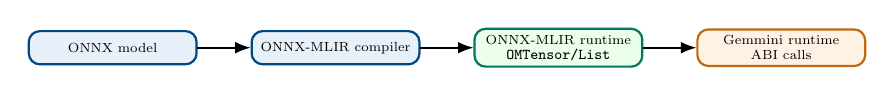
\begin{tikzpicture}[
    scale=0.68,
    every node/.style={transform shape},
    box/.style={rectangle,rounded corners,draw=ieeeblue,fill=ieeelight,thick,
      text width=2.9cm,minimum height=0.62cm,align=center,font=\scriptsize},
    rt/.style={rectangle,rounded corners,draw=stagegreen,fill=green!8,thick,
      text width=2.9cm,minimum height=0.62cm,align=center,font=\scriptsize},
    gem/.style={rectangle,rounded corners,draw=stageorange,fill=orange!10,thick,
      text width=2.9cm,minimum height=0.62cm,align=center,font=\scriptsize},
    arrow/.style={-{Latex[length=2mm]},thick}
  ]
    \node[box] (onnx) {ONNX model};
    \node[box,right=of onnx] (compiler) {ONNX-MLIR compiler};
    \node[rt,right=of compiler] (omrt) {ONNX-MLIR runtime\\\code{OMTensor/List}};
    \node[gem,right=of omrt] (gemrt) {Gemmini runtime\\ABI calls};
    \draw[arrow] (onnx) -- (compiler);
    \draw[arrow] (compiler) -- (omrt);
    \draw[arrow] (omrt) -- (gemrt);
  \end{tikzpicture}
  \vspace{0.2em}
  {\tiny\color{codegray}
  In this deck, ``runtime'' usually means ONNX-MLIR runtime plus Gemmini runtime linked into the compiled executable, not Microsoft ONNX Runtime.}
\end{frame}

% 5j
\begin{frame}{Why ONNX Runtime Is Not Used Here}
  \centering
  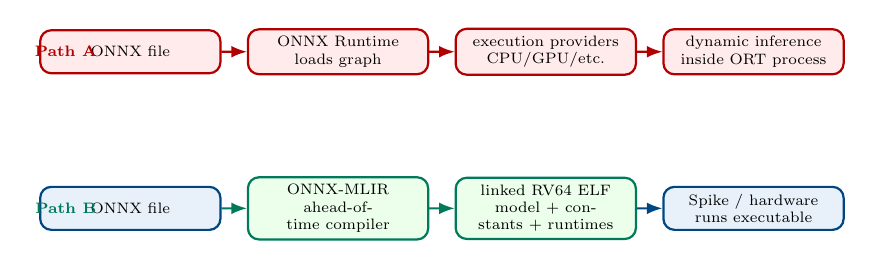
\begin{tikzpicture}[
    scale=0.78,
    every node/.style={transform shape},
    node distance=0.42cm,
    ort/.style={rectangle,rounded corners,draw=red!70!black,fill=red!8,thick,
      text width=2.7cm,minimum height=0.7cm,align=center,font=\scriptsize},
    comp/.style={rectangle,rounded corners,draw=stagegreen,fill=green!8,thick,
      text width=2.7cm,minimum height=0.7cm,align=center,font=\scriptsize},
    bin/.style={rectangle,rounded corners,draw=ieeeblue,fill=ieeelight,thick,
      text width=2.7cm,minimum height=0.7cm,align=center,font=\scriptsize},
    arrow/.style={-{Latex[length=2mm]},thick}
  ]
    \node[ort] (onnx1) at (0,1.2) {ONNX file};
    \node[ort,right=of onnx1] (ort) {ONNX Runtime\\loads graph};
    \node[ort,right=of ort] (providers) {execution providers\\CPU/GPU/etc.};
    \node[ort,right=of providers] (run1) {dynamic inference\\inside ORT process};

    \node[bin] (onnx2) at (0,-1.35) {ONNX file};
    \node[comp,right=of onnx2] (compiler) {ONNX-MLIR\\ahead-of-time compiler};
    \node[comp,right=of compiler] (elf) {linked RV64 ELF\\model + constants + runtimes};
    \node[bin,right=of elf] (run2) {Spike / hardware\\runs executable};

    \draw[arrow,draw=red!70!black] (onnx1) -- (ort);
    \draw[arrow,draw=red!70!black] (ort) -- (providers);
    \draw[arrow,draw=red!70!black] (providers) -- (run1);

    \draw[arrow,draw=stagegreen] (onnx2) -- (compiler);
    \draw[arrow,draw=stagegreen] (compiler) -- (elf);
    \draw[arrow,draw=ieeeblue] (elf) -- (run2);

    \node[font=\scriptsize\bfseries\color{red!70!black}] at (-1.05,1.2) {Path A};
    \node[font=\scriptsize\bfseries\color{stagegreen}] at (-1.05,-1.35) {Path B};
  \end{tikzpicture}

  \vspace{0.55em}
  \scriptsize
  \begin{tabularx}{\textwidth}{@{}lX@{}}
    \toprule
    Question & Answer for this project \\
    \midrule
    \edgeword{Why not ONNX Runtime?} &
      Because after compilation there is no ONNX graph to interpret at execution time. The model has already become RV64 code, constants, runtime calls, and Gemmini custom instructions. \\
    \edgeword{What replaces it?} &
      The linked executable uses ONNX-MLIR runtime for \code{OMTensor}/\code{OMTensorList} and Gemmini runtime for accelerator kernels. \\
    \edgeword{What would ONNX Runtime do?} &
      It would load the original \code{.onnx} model and dispatch nodes through its own execution-provider system. That is a different execution architecture from this AOT Gemmini binary. \\
    \bottomrule
  \end{tabularx}
\end{frame}

% 5k
\begin{frame}{What Breaks If We Expect ONNX Runtime Here?}
  \scriptsize
  \begin{tabularx}{\textwidth}{@{}lX@{}}
    \toprule
    Confusion & Clear mental model \\
    \midrule
    \edgeword{``The binary should call ONNX Runtime.''} &
      No. The binary calls generated functions and runtime helpers such as \code{om\_gemmini\_conv\_f32}. ONNX Runtime APIs like \code{OrtSession} are not part of this RV64/Gemmini path. \\
    \edgeword{``ONNX Runtime will choose Gemmini.''} &
      No. Gemmini selection happens during ONNX-MLIR lowering passes, before the final executable is linked. \\
    \edgeword{``The \code{.onnx} file is needed at inference time.''} &
      No. The final executable already contains model code and constants. The ONNX file is an input to compilation, not an input to the deployed RV64 binary. \\
    \edgeword{``Runtime means ONNX Runtime.''} &
      Not in this deck. Here, runtime means the small support code linked with compiled model code: ONNX-MLIR runtime plus Gemmini runtime. \\
    \bottomrule
  \end{tabularx}

  \vspace{0.55em}
  \begin{block}{Short rule}
    ONNX Runtime executes ONNX models dynamically. ONNX-MLIR produces an executable ahead of time. This project is the second path.
  \end{block}
\end{frame}

% 5l
\begin{frame}{Utility of ONNX Runtime}
  \scriptsize
  \begin{block}{Simple definition}
    ONNX Runtime is useful when the deployment goal is: load a \code{model.onnx} file at execution time, choose kernels dynamically, and run inference through an inference engine.
  \end{block}

  \vspace{0.25em}
  \begin{tabularx}{\textwidth}{@{}lX@{}}
    \toprule
    Utility & Meaning \\
    \midrule
    \edgeword{Direct ONNX execution} &
      It reads the ONNX graph at runtime and executes nodes without first producing a standalone compiler-generated executable. \\
    \edgeword{Execution providers} &
      It can dispatch work to CPU, CUDA, TensorRT, DirectML, and other provider backends depending on the installed platform. \\
    \edgeword{Flexible deployment} &
      The same \code{.onnx} model can be moved between machines and providers without rebuilding a target-specific binary each time. \\
    \edgeword{Runtime services} &
      It handles graph loading, operator scheduling, kernel dispatch, memory planning, and model session APIs. \\
    \bottomrule
  \end{tabularx}

  \vspace{0.35em}
  \begin{center}
    \code{model.onnx} \quad$\rightarrow$\quad \code{ONNX Runtime} \quad$\rightarrow$\quad inference result
  \end{center}
\end{frame}

% 5m
\begin{frame}{Can We Use ONNX Runtime in Our Gemmini Case?}
  \scriptsize
  \begin{tabularx}{\textwidth}{@{}lXX@{}}
    \toprule
    Use & Yes / No & Explanation \\
    \midrule
    \edgeword{Final RV64/Gemmini execution} &
      No &
      The final executable does not load \code{model.onnx}; it runs compiled RV64 code and calls ONNX-MLIR/Gemmini runtime functions. \\
    \edgeword{CPU baseline} &
      Yes &
      Run the same \code{resnet18.onnx} with ONNX Runtime on CPU and compare outputs or timing against the Gemmini binary. \\
    \edgeword{Golden reference output} &
      Yes &
      Use ONNX Runtime to generate expected output tensors, then check whether Gemmini output matches. \\
    \edgeword{Model validity check} &
      Yes &
      If ONNX-MLIR or Gemmini lowering fails, ONNX Runtime can confirm whether the original ONNX model itself is valid. \\
    \edgeword{Direct Gemmini provider} &
      Not currently &
      That would require a custom ONNX Runtime Execution Provider for Gemmini. This project instead uses ONNX-MLIR AOT compilation. \\
    \bottomrule
  \end{tabularx}
\end{frame}

% 5n
\begin{frame}{Compare ONNX Runtime and ONNX-MLIR Runtime}
  \scriptsize
  \begin{tabularx}{\textwidth}{@{}lXX@{}}
    \toprule
    Point & ONNX Runtime & ONNX-MLIR Runtime \\
    \midrule
    \edgeword{Main role} & Runs \code{.onnx} models directly. & Supports code generated by ONNX-MLIR. \\
    \edgeword{Execution style} & Dynamic inference engine. & Linked support library for compiled model execution. \\
    \edgeword{Inference input} & \code{model.onnx}. & Compiled binary/shared library plus user input tensors. \\
    \edgeword{Who reads graph?} & ONNX Runtime reads the graph at runtime. & ONNX-MLIR compiler reads the graph before runtime. \\
    \edgeword{Kernel choice} & Runtime chooses kernels/providers. & Compiler/lowering already selected calls and code paths. \\
    \edgeword{Gemmini path} & Would need a Gemmini Execution Provider. & Uses generated code, Gemmini runtime, and Gemmini ABI. \\
    \edgeword{Our project} & Useful as CPU/reference baseline. & Required for \code{OMTensor}, \code{OMTensorList}, and compiled model support. \\
    \bottomrule
  \end{tabularx}

  \vspace{0.35em}
  \begin{center}
    \code{ONNX Runtime = dynamic ONNX inference} \qquad
    \code{ONNX-MLIR Runtime = support for compiled ONNX}
  \end{center}
\end{frame}

% 5o
\begin{frame}{Why ONNX-MLIR Avoids Depending on ONNX Runtime}
  \scriptsize
  \begin{tabularx}{\textwidth}{@{}lX@{}}
    \toprule
    Reason & Explanation \\
    \midrule
    \edgeword{Ahead-of-time compilation} &
      ONNX-MLIR wants the ONNX graph compiled before execution, not interpreted at execution time. \\
    \edgeword{Compiler optimizations} &
      It can lower operations into loops, LLVM IR, target-specific calls, and accelerator instructions. \\
    \edgeword{Smaller deployment dependency} &
      The final program needs only compiled model code and support runtimes, not a full ONNX inference engine. \\
    \edgeword{Hardware backend control} &
      Compiler passes can target CPUs, IBM NNPA, Gemmini, or other accelerators directly through lowering and ABI code. \\
    \edgeword{Static embedded path} &
      A standalone RV64 binary is easier to run on Spike, FPGA SoCs, or constrained systems than a dynamic ONNX Runtime stack. \\
    \edgeword{Clear ABI} &
      Generated code calls known functions such as \code{om\_gemmini\_conv\_f32}; hardware commands are emitted through \code{gemmini.h}. \\
    \bottomrule
  \end{tabularx}

  \vspace{0.35em}
  \begin{block}{Important}
    ONNX Runtime is not bad or useless globally. It is simply the wrong execution architecture for this AOT Gemmini compiler pipeline.
  \end{block}
\end{frame}

% 5p
\begin{frame}{Why Our Path Is Better for Gemmini}
  \scriptsize
  \begin{block}{Scope}
    This does not mean ONNX-MLIR is always better than ONNX Runtime. It means ONNX-MLIR is better for this Gemmini/RV64 accelerator pipeline.
  \end{block}

  \vspace{0.25em}
  \begin{tabularx}{\textwidth}{@{}lX@{}}
    \toprule
    Advantage & Why it matters for Gemmini \\
    \midrule
    \edgeword{Direct hardware targeting} &
      Conv and MatMul can lower into Gemmini runtime calls, RoCC custom instructions, and Gemmini ABI commands. \\
    \edgeword{Ahead-of-time binary} &
      Spike or hardware runs a normal RV64 ELF; it does not need to load or interpret an ONNX graph. \\
    \edgeword{Compiler visibility} &
      ONNX-MLIR can inspect, rewrite, lower, tile, and specialize operations before inference starts. \\
    \edgeword{Smaller execution stack} &
      The final path links only needed support code instead of carrying a full dynamic inference engine. \\
    \edgeword{ABI control} &
      We control the exact boundary from generated code to \code{om\_gemmini\_conv\_f32}, then to \code{gemmini.h} custom instructions. \\
    \edgeword{Research extensibility} &
      New dialects, passes, lowering rules, and Gemmini-specific optimizations can be added inside the compiler pipeline. \\
    \bottomrule
  \end{tabularx}

  \vspace{0.35em}
  \begin{center}
    \code{ONNX Runtime = flexible general inference engine}\\
    \code{ONNX-MLIR + Gemmini = specialized compiler path for hardware acceleration}
  \end{center}
\end{frame}

% 5q
\begin{frame}{When to Choose Each Path}
  \scriptsize
  \begin{tabularx}{\textwidth}{@{}lXX@{}}
    \toprule
    Choose & Best target environment & Why \\
    \midrule
    \edgeword{ONNX Runtime + Custom EP} &
      Cloud servers, PCs, and powerful edge systems such as Jetson-class devices. &
      RAM is usually not the main constraint, models may change frequently, and dynamic provider dispatch is useful. \\
    \edgeword{ONNX-MLIR} &
      Proprietary ASIC/FPGA accelerators, critical embedded systems, RISC-V SoCs, and IoT processors. &
      Every kilobyte matters, the target hardware is highly specific, and raw execution speed matters more than software flexibility. \\
    \bottomrule
  \end{tabularx}

  \vspace{0.55em}
  \begin{block}{Decision rule}
    ONNX Runtime is the strong default for standard cloud inference. ONNX-MLIR is preferred when the goal is to remove software overhead and produce maximum raw performance on highly specialized hardware.
  \end{block}

  \vspace{0.35em}
  \begin{center}
    \code{Custom EP path = flexible engine}\\
    \code{ONNX-MLIR path = compiled hardware-specific executable}
  \end{center}
\end{frame}

% 5r
\begin{frame}{Hailo Pipeline: AOT Compiler Suite Example}
  \centering
  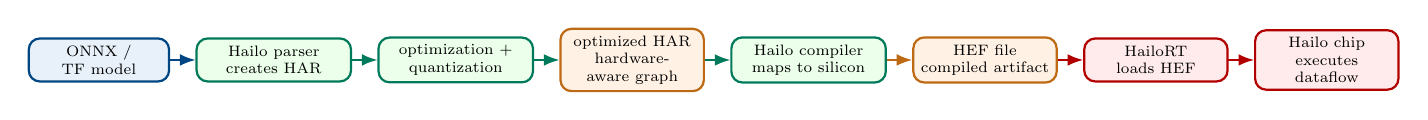
\begin{tikzpicture}[
    scale=0.78,
    every node/.style={transform shape},
    node distance=0.42cm,
    src/.style={rectangle,rounded corners,draw=ieeeblue,fill=ieeelight,thick,
      text width=2.05cm,minimum height=0.70cm,align=center,font=\scriptsize},
    comp/.style={rectangle,rounded corners,draw=stagegreen,fill=green!8,thick,
      text width=2.28cm,minimum height=0.70cm,align=center,font=\scriptsize},
    art/.style={rectangle,rounded corners,draw=stageorange,fill=orange!10,thick,
      text width=2.10cm,minimum height=0.70cm,align=center,font=\scriptsize},
    rt/.style={rectangle,rounded corners,draw=red!70!black,fill=red!8,thick,
      text width=2.10cm,minimum height=0.70cm,align=center,font=\scriptsize},
    arrow/.style={-{Latex[length=2mm]},thick}
  ]
    \node[src] (onnx) {ONNX / TF model};
    \node[comp,right=of onnx] (parse) {Hailo parser\\creates HAR};
    \node[comp,right=of parse] (opt) {optimization +\\quantization};
    \node[art,right=of opt] (har) {optimized HAR\\hardware-aware graph};
    \node[comp,right=of har] (compile) {Hailo compiler\\maps to silicon};
    \node[art,right=of compile] (hef) {HEF file\\compiled artifact};
    \node[rt,right=of hef] (hailort) {HailoRT\\loads HEF};
    \node[rt,right=of hailort] (chip) {Hailo chip\\executes dataflow};

    \draw[arrow,draw=ieeeblue] (onnx) -- (parse);
    \draw[arrow,draw=stagegreen] (parse) -- (opt);
    \draw[arrow,draw=stagegreen] (opt) -- (har);
    \draw[arrow,draw=stagegreen] (har) -- (compile);
    \draw[arrow,draw=stageorange] (compile) -- (hef);
    \draw[arrow,draw=red!70!black] (hef) -- (hailort);
    \draw[arrow,draw=red!70!black] (hailort) -- (chip);
  \end{tikzpicture}

  \vspace{0.55em}
  \scriptsize
  \begin{block}{What this shows}
    Hailo uses an ahead-of-time compiler flow: the model is parsed, optimized, quantized, mapped onto the physical dataflow resources of the chip, and emitted as a fixed compiled artifact. Production inference loads the compiled artifact; it does not need ONNX Runtime to interpret the original graph.
  \end{block}

  \vspace{0.2em}
  {\tiny Sources:
  \href{https://hailo.ai/developer-zone/documentation/}{Hailo Developer Zone documentation}
  \quad|\quad
  \href{https://github.com/hailo-ai/hailo_model_zoo}{Hailo Model Zoo}}
\end{frame}

% 5s
\begin{frame}{Hailo and ONNX-MLIR Share the Same Compiler Philosophy}
  \centering
  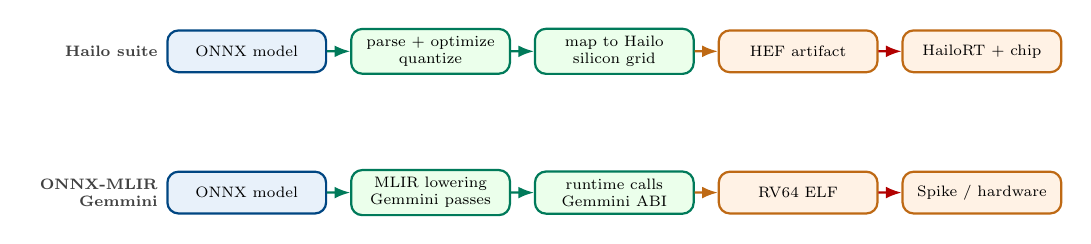
\begin{tikzpicture}[
    scale=0.78,
    every node/.style={transform shape},
    node distance=0.38cm,
    label/.style={font=\scriptsize\bfseries,text=codegray,align=right,text width=2.0cm},
    box/.style={rectangle,rounded corners,draw=ieeeblue,fill=ieeelight,thick,
      text width=2.35cm,minimum height=0.68cm,align=center,font=\scriptsize},
    comp/.style={rectangle,rounded corners,draw=stagegreen,fill=green!8,thick,
      text width=2.35cm,minimum height=0.68cm,align=center,font=\scriptsize},
    artifact/.style={rectangle,rounded corners,draw=stageorange,fill=orange!10,thick,
      text width=2.35cm,minimum height=0.68cm,align=center,font=\scriptsize},
    arrow/.style={-{Latex[length=2mm]},thick}
  ]
    \node[label] at (-1.0,1.15) {Hailo suite};
    \node[box] (h1) at (1.45,1.15) {ONNX model};
    \node[comp,right=of h1] (h2) {parse + optimize\\quantize};
    \node[comp,right=of h2] (h3) {map to Hailo\\silicon grid};
    \node[artifact,right=of h3] (h4) {HEF artifact};
    \node[artifact,right=of h4] (h5) {HailoRT + chip};

    \node[label] at (-1.0,-1.15) {ONNX-MLIR\\Gemmini};
    \node[box] (g1) at (1.45,-1.15) {ONNX model};
    \node[comp,right=of g1] (g2) {MLIR lowering\\Gemmini passes};
    \node[comp,right=of g2] (g3) {runtime calls\\Gemmini ABI};
    \node[artifact,right=of g3] (g4) {RV64 ELF};
    \node[artifact,right=of g4] (g5) {Spike / hardware};

    \draw[arrow,draw=stagegreen] (h1) -- (h2);
    \draw[arrow,draw=stagegreen] (h2) -- (h3);
    \draw[arrow,draw=stageorange] (h3) -- (h4);
    \draw[arrow,draw=red!70!black] (h4) -- (h5);

    \draw[arrow,draw=stagegreen] (g1) -- (g2);
    \draw[arrow,draw=stagegreen] (g2) -- (g3);
    \draw[arrow,draw=stageorange] (g3) -- (g4);
    \draw[arrow,draw=red!70!black] (g4) -- (g5);
  \end{tikzpicture}

  \vspace{0.55em}
  \scriptsize
  \begin{tabularx}{\textwidth}{@{}lX@{}}
    \toprule
    Shared idea & Explanation \\
    \midrule
    \edgeword{AOT compilation} &
      Both paths move expensive graph analysis and hardware mapping before deployment. \\
    \edgeword{No production ONNX graph interpreter} &
      In production, Hailo loads HEF and ONNX-MLIR/Gemmini runs an ELF; neither path needs ONNX Runtime to interpret the original ONNX graph. \\
    \edgeword{Hardware-specific artifact} &
      Hailo emits an artifact for Hailo silicon; ONNX-MLIR/Gemmini emits code and ABI calls for RISC-V + Gemmini. \\
    \bottomrule
  \end{tabularx}
\end{frame}

% 5t
\begin{frame}[fragile]{Mirror Code: HailoRT vs ONNX-MLIR Runtime}
  \scriptsize
  \begin{columns}[T,onlytextwidth]
    \begin{column}{0.48\textwidth}
      \begin{block}{HailoRT idea}
        Python loads a compiled \edgeword{HEF} artifact, opens hardware streams, and pushes preprocessed tensors toward the Hailo NPU.
      \end{block}
      \centering
      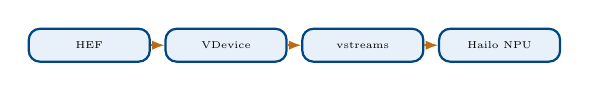
\begin{tikzpicture}[
        scale=0.72,
        every node/.style={transform shape},
        node distance=0.25cm,
        flowbox/.style={rectangle,rounded corners,draw=ieeeblue,fill=ieeelight,thick,
          text width=1.9cm,minimum height=0.58cm,align=center,font=\tiny},
        arrow/.style={-{Latex[length=1.6mm]},thick,draw=stageorange}
      ]
        \node[flowbox] (hef) {HEF};
        \node[flowbox,right=of hef] (vdev) {VDevice};
        \node[flowbox,right=of vdev] (stream) {vstreams};
        \node[flowbox,right=of stream] (npu) {Hailo NPU};
        \draw[arrow] (hef) -- (vdev);
        \draw[arrow] (vdev) -- (stream);
        \draw[arrow] (stream) -- (npu);
      \end{tikzpicture}
    \end{column}
    \begin{column}{0.50\textwidth}
      \begin{block}{Equivalent ONNX-MLIR PyRuntime idea}
        Python loads a compiled \edgeword{.so} artifact and calls native compiled model code through \code{OMExecutionSession}.
      \end{block}
\begin{lstlisting}[language=Python]
import numpy as np
import cv2
from PyRuntime import OMExecutionSession

SO_FILE = "my_compiled_model.so"   # like Hailo .hef
IMAGE_FILE = "test_image.jpg"

session = OMExecutionSession(SO_FILE)

batch, channels, height, width = 1, 3, 224, 224
img = cv2.imread(IMAGE_FILE)
img = cv2.resize(img, (width, height))
img = cv2.cvtColor(img, cv2.COLOR_BGR2RGB)
img = img.transpose(2, 0, 1)       # NHWC -> NCHW
input_data = np.ascontiguousarray(
    np.expand_dims(img, axis=0), dtype=np.float32)

outputs = session.run([input_data])
print(outputs[0].shape)
\end{lstlisting}
    \end{column}
  \end{columns}

  \vspace{0.25em}
  {\tiny
  In both versions, Python is only the host-side plumbing: it prepares NumPy memory and sends it into a compiled black box. No runtime loop inspects the ONNX graph during inference.}
\end{frame}

% 5u
\begin{frame}{What Changes Between HailoRT and ONNX-MLIR Runtime}
  \scriptsize
  \begin{tabularx}{\textwidth}{@{}lXX@{}}
    \toprule
    Logical step & HailoRT inference on NPU & ONNX-MLIR Runtime inference on compiled \code{.so} \\
    \midrule
    \edgeword{Binary artifact} &
      \code{.hef}: a spatial dataflow configuration compiled for Hailo silicon. &
      \code{.so} / \code{.dll}: native machine-code library produced by ONNX-MLIR. \\
    \edgeword{Hardware setup} &
      \code{VDevice()} initializes the physical NPU through PCIe, USB, or the platform driver. &
      \code{OMExecutionSession()} loads the shared library into RAM and prepares calls into compiled model code. \\
    \edgeword{Tensor layout} &
      Often \code{NHWC}, because vision accelerators like contiguous pixel streams. &
      Often \code{NCHW}, the common ONNX/PyTorch-style layout, so image data may need transposition. \\
    \edgeword{Data type} &
      Usually \code{uint8} or \code{int8}; quantization is part of the hardware contract. &
      Usually \code{float32} unless the model and compiler flow are explicitly quantized. \\
    \edgeword{Data transfer} &
      \code{input\_vstreams[0].write(data)} pushes bytes into hardware stream/DMA channels. &
      \code{session.run([data])} converts NumPy arrays to internal OMTensors and calls compiled C entry points. \\
    \bottomrule
  \end{tabularx}

  \vspace{0.45em}
  \begin{block}{Conclusion}
    Both paths use the same AOT philosophy: the compiler resolves graph structure before deployment. Runtime code only injects tensors into a fast compiled artifact, not into a graph interpreter.
  \end{block}
\end{frame}

% 5t
\begin{frame}{Engine vs Interface: Runtime Mental Model}
  \scriptsize
  \begin{tabularx}{\textwidth}{@{}lXX@{}}
    \toprule
    Runtime & Analogy & Technical meaning \\
    \midrule
    \edgeword{ONNX Runtime} &
      A large factory engine. You give it the machine plan, the \code{.onnx} file. It loads the plan, prepares tools, schedules work, and runs the gears for every inference. &
      A full inference framework: graph loader, optimizer, scheduler, execution-provider dispatcher, kernel library, and session API. \\
    \edgeword{ONNX-MLIR Runtime} &
      A small funnel attached to a pre-molded metal block. The compiler already shaped the block, the \code{.so}, \code{.jar}, or executable. The runtime only feeds data into it cleanly. &
      A lightweight interface library: passes tensors between user code and compiled model code using structures such as \code{OMTensor} and \code{OMTensorList}. \\
    \bottomrule
  \end{tabularx}

  \vspace{0.55em}
  \begin{block}{For Gemmini}
    The Gemmini binary should behave like the pre-molded block: compiled code, constants, runtime wrappers, and hardware ABI calls are already prepared before execution.
  \end{block}
\end{frame}

% 6
\begin{frame}{LLVM Carries Typed Code Toward RV64}
  \begin{columns}
    \begin{column}{0.47\textwidth}
      \centering
      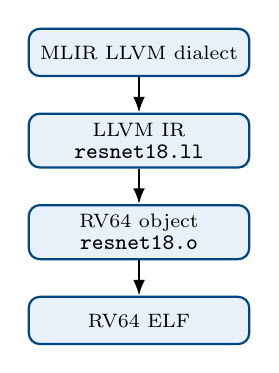
\begin{tikzpicture}[node distance=0.45cm, every node/.style={transform shape},
        box/.style={rectangle,rounded corners,draw=ieeeblue,fill=ieeelight,thick,
          minimum width=2.8cm,minimum height=0.6cm,align=center,font=\scriptsize},
        arrow/.style={-{Latex[length=2mm]},thick}]
        \node[box] (mlir) {MLIR LLVM dialect};
        \node[box,below=of mlir] (ir) {LLVM IR\\\code{resnet18.ll}};
        \node[box,below=of ir] (obj) {RV64 object\\\code{resnet18.o}};
        \node[box,below=of obj] (elf) {RV64 ELF};
        \draw[arrow] (mlir) -- (ir);
        \draw[arrow] (ir) -- (obj);
        \draw[arrow] (obj) -- (elf);
      \end{tikzpicture}
    \end{column}
    \begin{column}{0.5\textwidth}
      \begin{block}{LLVM}
        Compiler layer that turns typed LLVM IR into target machine code.
      \end{block}
      \begin{itemize}
        \item Every value in LLVM IR has a type.
        \item Examples: \code{i64}, \code{float}, \code{ptr}, \code{void}.
        \item Function calls must match declared argument types.
        \item \code{llc} emits RV64 object code.
        \item Target: \code{riscv64-unknown-linux-gnu}.
      \end{itemize}
      \withoutit{the compiler would not have a typed, target-independent handoff to produce RV64 object code. Runtime calls and data pointers would be much easier to miscompile.}
    \end{column}
  \end{columns}
\end{frame}

% 6b
\begin{frame}[fragile]{How LLVM Types Protect Runtime Calls}
  \begin{columns}[T]
    \begin{column}{0.52\textwidth}
      \begin{lstlisting}
declare void @om_gemmini_conv_f32(
  ptr, ptr, ptr, i64, i64)

call void @om_gemmini_conv_f32(
  ptr %16, ptr %25, ptr %34,
  i64 2, i64 3)
      \end{lstlisting}
    \end{column}
    \begin{column}{0.45\textwidth}
      \begin{block}{Typed Means Explicit Shape of Values}
        LLVM does not see only names. It sees what binary kind each value has.
      \end{block}
      \begin{itemize}
        \item \code{void}: function returns no value.
        \item \code{ptr}: address of an \code{OMTensor} descriptor.
        \item \code{i64}: 64-bit integer, used here for stride and padding.
        \item \code{float}: 32-bit floating-point data in constants.
      \end{itemize}
    \end{column}
  \end{columns}
\end{frame}

% 6c
\begin{frame}{Why Typed Calls Matter}
  \centering
  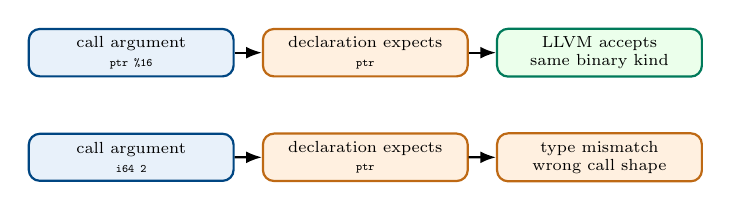
\begin{tikzpicture}[
    scale=0.83,
    every node/.style={transform shape},
    node distance=0.42cm,
    box/.style={rectangle,rounded corners,draw=ieeeblue,fill=ieeelight,thick,
      text width=2.9cm,minimum height=0.72cm,align=center,font=\scriptsize},
    type/.style={rectangle,rounded corners,draw=stageorange,fill=orange!12,thick,
      text width=2.9cm,minimum height=0.72cm,align=center,font=\scriptsize},
    ok/.style={rectangle,rounded corners,draw=stagegreen,fill=green!8,thick,
      text width=2.9cm,minimum height=0.72cm,align=center,font=\scriptsize},
    arrow/.style={-{Latex[length=2mm]},thick}
  ]
    \node[box] (call) {call argument\\\tinycode{ptr \%16}};
    \node[type,right=of call] (decl) {declaration expects\\\tinycode{ptr}};
    \node[ok,right=of decl] (ok) {LLVM accepts\\same binary kind};
    \node[box,below=0.85cm of call] (bad) {call argument\\\tinycode{i64 2}};
    \node[type,right=of bad] (baddecl) {declaration expects\\\tinycode{ptr}};
    \node[type,right=of baddecl] (reject) {type mismatch\\wrong call shape};

    \draw[arrow] (call) -- (decl);
    \draw[arrow] (decl) -- (ok);
    \draw[arrow] (bad) -- (baddecl);
    \draw[arrow] (baddecl) -- (reject);
  \end{tikzpicture}

  \vspace{0.4em}
  \begin{block}{In This Project}
    LLVM types make the runtime boundary explicit: three tensor descriptor addresses, then two 64-bit convolution parameters.
  \end{block}
\end{frame}

% 6d
\begin{frame}{llc Turns LLVM IR into RV64 Objects}
  \begin{columns}
    \begin{column}{0.44\textwidth}
      \centering
      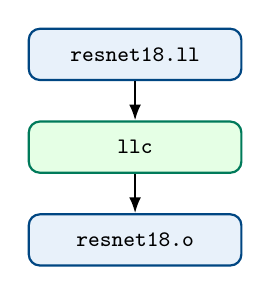
\begin{tikzpicture}[node distance=0.5cm, every node/.style={transform shape},
        box/.style={rectangle,rounded corners,draw=ieeeblue,fill=ieeelight,thick,
          minimum width=2.7cm,minimum height=0.65cm,align=center,font=\scriptsize},
        tool/.style={rectangle,rounded corners,draw=stagegreen,fill=green!10,thick,
          minimum width=2.7cm,minimum height=0.65cm,align=center,font=\scriptsize},
        arrow/.style={-{Latex[length=2mm]},thick}]
        \node[box] (in) {\code{resnet18.ll}};
        \node[tool,below=of in] (llc) {\code{llc}};
        \node[box,below=of llc] (out) {\code{resnet18.o}};
        \draw[arrow] (in) -- (llc);
        \draw[arrow] (llc) -- (out);
      \end{tikzpicture}
    \end{column}
    \begin{column}{0.53\textwidth}
      \begin{block}{LLVM Static Compiler}
        \code{llc} lowers LLVM IR into target assembly or object code.
      \end{block}
      \begin{itemize}
        \item Input: \code{resnet18.ll}.
        \item Output: relocatable RV64 object.
        \item Runtime symbols are resolved later by the linker.
      \end{itemize}
      \withoutit{\code{resnet18.ll} remains compiler IR. The model cannot become \code{resnet18.o}, so the linker cannot produce the final RV64 executable.}
    \end{column}
  \end{columns}
\end{frame}

% 7
\begin{frame}{MLIR Keeps Multiple Abstraction Levels}
  \begin{columns}
    \begin{column}{0.5\textwidth}
      \centering
      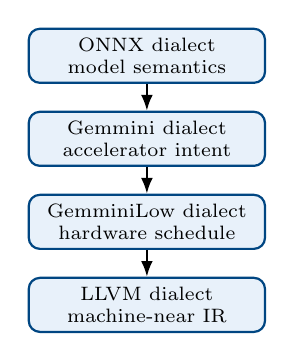
\begin{tikzpicture}[node distance=0.34cm, every node/.style={transform shape},
        box/.style={rectangle,rounded corners,draw=ieeeblue,fill=ieeelight,thick,
          minimum width=3.0cm,minimum height=0.52cm,align=center,font=\scriptsize},
        arrow/.style={-{Latex[length=2mm]},thick}]
        \node[box] (a) {ONNX dialect\\model semantics};
        \node[box,below=of a] (b) {Gemmini dialect\\accelerator intent};
        \node[box,below=of b] (c) {GemminiLow dialect\\hardware schedule};
        \node[box,below=of c] (d) {LLVM dialect\\machine-near IR};
        \draw[arrow] (a) -- (b);
        \draw[arrow] (b) -- (c);
        \draw[arrow] (c) -- (d);
      \end{tikzpicture}
    \end{column}
    \begin{column}{0.47\textwidth}
      \begin{block}{Multi-Level IR}
        MLIR represents the same program at multiple abstraction levels.
      \end{block}
      \begin{itemize}
        \item High level: ONNX graph ops.
        \item Middle: accelerator intent.
        \item Low: hardware and binary details.
      \end{itemize}
      \withoutit{all compiler stages would need one flat representation. ONNX semantics, Gemmini intent, and hardware details would be mixed and difficult to verify or rewrite safely.}
    \end{column}
  \end{columns}
\end{frame}

% 8
\begin{frame}{Dialects Give Each Level Its Own Language}
  \begin{columns}
    \begin{column}{0.48\textwidth}
      \centering
      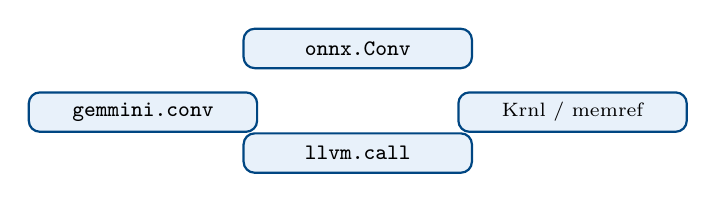
\begin{tikzpicture}[node distance=0.25cm, every node/.style={transform shape},
        box/.style={rectangle,rounded corners,draw=ieeeblue,fill=ieeelight,thick,
          minimum width=2.9cm,minimum height=0.5cm,align=center,font=\scriptsize}]
        \node[box] (o) {\code{onnx.Conv}};
        \node[box,below left=0.28cm and -0.2cm of o] (g) {\code{gemmini.conv}};
        \node[box,below right=0.28cm and -0.2cm of o] (k) {Krnl / memref};
        \node[box,below=0.8cm of o] (l) {\code{llvm.call}};
      \end{tikzpicture}
    \end{column}
    \begin{column}{0.49\textwidth}
      \begin{block}{Dialect}
        Namespace of MLIR operations, attributes, and types for one domain.
      \end{block}
      \begin{itemize}
        \item ONNX: model semantics.
        \item Gemmini: accelerator semantics.
        \item GemminiLow: hardware actions.
        \item LLVM: machine-near calls and types.
      \end{itemize}
      \withoutit{operations would have no clear namespace or rules. A pass could confuse model-level Conv with hardware-level load/execute/store details.}
    \end{column}
  \end{columns}
\end{frame}

% 8b
\begin{frame}{How Dialects Map to Pipeline Stages}
  \scriptsize
  \begin{tabularx}{\textwidth}{@{}lX@{}}
    \toprule
    Dialect / Layer & Example Meaning \\
    \midrule
    ONNX & \code{onnx.Conv}: neural-network graph convolution. \\
    Krnl & ONNX-MLIR kernel dialect: loops, \code{memref} buffers, allocations, constants, and runtime-call setup before LLVM. \\
    Gemmini & Accelerator intent: this operation is selected for Gemmini. \\
    GemminiLow & Hardware-level schedule: configure, load, execute, store. \\
    LLVM dialect & MLIR representation close to LLVM IR. \\
    LLVM IR & Textual LLVM form consumed by LLVM tools. \\
    RV64 ELF & Final executable binary for Spike or hardware. \\
    \bottomrule
  \end{tabularx}
\end{frame}

% 9
\begin{frame}{Conversion Chooses the Next Representation}
  \begin{columns}
    \begin{column}{0.48\textwidth}
      \centering
      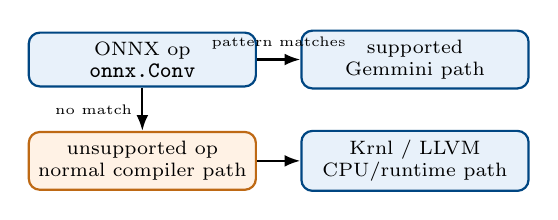
\begin{tikzpicture}[node distance=0.55cm, every node/.style={transform shape},
        box/.style={rectangle,rounded corners,draw=ieeeblue,fill=ieeelight,thick,
          text width=2.65cm,minimum height=0.62cm,align=center,font=\scriptsize},
        fallback/.style={rectangle,rounded corners,draw=stageorange,fill=orange!10,thick,
          text width=2.65cm,minimum height=0.62cm,align=center,font=\scriptsize},
        arrow/.style={-{Latex[length=2mm]},thick}]
        \node[box] (a) {ONNX op\\\code{onnx.Conv}};
        \node[box,right=of a] (b) {supported\\Gemmini path};
        \node[fallback,below=of a] (f) {unsupported op\\normal compiler path};
        \node[box,right=of f] (k) {Krnl / LLVM\\CPU/runtime path};
        \draw[arrow] (a) -- node[above,font=\tiny]{pattern matches} (b);
        \draw[arrow] (a) -- node[left,font=\tiny]{no match} (f);
        \draw[arrow] (f) -- (k);
      \end{tikzpicture}
    \end{column}
    \begin{column}{0.49\textwidth}
      \begin{block}{Conversion}
        Tries to rewrite an operation when a valid pattern exists.
      \end{block}
      \begin{itemize}
        \item A pattern says: this source op can become that target op.
        \item Legality checks shape, type, padding, stride, and attributes.
        \item If no safe Gemmini pattern exists, the op stays on the standard lowering path.
      \end{itemize}
      \withoutit{ONNX operations would stay in the wrong form. Supported Conv could not become Gemmini code, and unsupported ops could not be separated cleanly for fallback.}
    \end{column}
  \end{columns}
\end{frame}

% 10
\begin{frame}{Fallback Preserves Correctness}
  \centering
  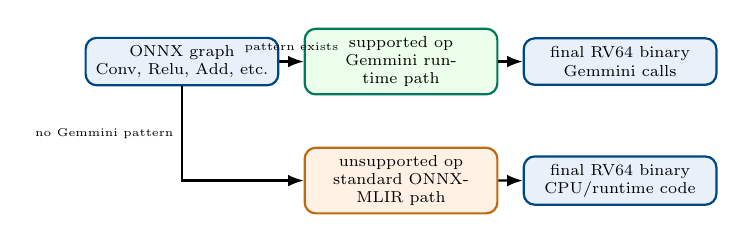
\begin{tikzpicture}[
    scale=0.82,
    every node/.style={transform shape},
    node distance=0.38cm,
    op/.style={rectangle,rounded corners,draw=ieeeblue,fill=ieeelight,thick,
      text width=2.75cm,minimum height=0.72cm,align=center,font=\scriptsize},
    gem/.style={rectangle,rounded corners,draw=stagegreen,fill=green!8,thick,
      text width=2.75cm,minimum height=0.72cm,align=center,font=\scriptsize},
    fall/.style={rectangle,rounded corners,draw=stageorange,fill=orange!10,thick,
      text width=2.75cm,minimum height=0.72cm,align=center,font=\scriptsize},
    arrow/.style={-{Latex[length=2mm]},thick}
  ]
    \node[op] (onnx) {ONNX graph\\Conv, Relu, Add, etc.};
    \node[gem,right=of onnx] (gemmini) {supported op\\Gemmini runtime path};
    \node[fall,below=0.8cm of gemmini] (fallback) {unsupported op\\standard ONNX-MLIR path};
    \node[op,right=of gemmini] (binaryA) {final RV64 binary\\Gemmini calls};
    \node[op,right=of fallback] (binaryB) {final RV64 binary\\CPU/runtime code};

    \draw[arrow] (onnx) -- node[above,font=\tiny] {pattern exists} (gemmini);
    \draw[arrow] (onnx) |- node[pos=0.25,left,font=\tiny] {no Gemmini pattern} (fallback);
    \draw[arrow] (gemmini) -- (binaryA);
    \draw[arrow] (fallback) -- (binaryB);
  \end{tikzpicture}

  \vspace{0.35em}
  \begin{block}{Meaning}
    Fallback means correctness first: unsupported operations are still compiled and executed, just not through Gemmini acceleration.
  \end{block}
  \withoutit{an unsupported operation might be forced into Gemmini incorrectly or dropped from the model. Fallback preserves correctness even when acceleration is not available.}
\end{frame}

% 10a
\begin{frame}{Lowering Moves Closer to Execution}
  \begin{columns}
    \begin{column}{0.50\textwidth}
      \centering
      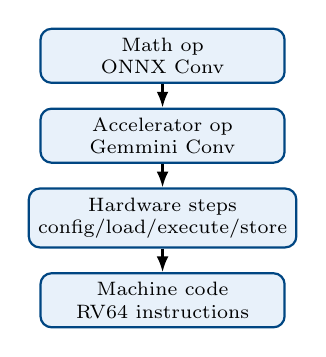
\begin{tikzpicture}[node distance=0.3cm, every node/.style={transform shape},
        box/.style={rectangle,rounded corners,draw=ieeeblue,fill=ieeelight,thick,
          minimum width=3.1cm,minimum height=0.5cm,align=center,font=\scriptsize},
        arrow/.style={-{Latex[length=2mm]},thick}]
        \node[box] (a) {Math op\\ONNX Conv};
        \node[box,below=of a] (b) {Accelerator op\\Gemmini Conv};
        \node[box,below=of b] (c) {Hardware steps\\config/load/execute/store};
        \node[box,below=of c] (d) {Machine code\\RV64 instructions};
        \draw[arrow] (a) -- (b);
        \draw[arrow] (b) -- (c);
        \draw[arrow] (c) -- (d);
      \end{tikzpicture}
    \end{column}
    \begin{column}{0.47\textwidth}
      \begin{block}{Lowering}
        Rewriting the same computation into a form with more execution details.
      \end{block}
      \begin{itemize}
        \item Preserves behavior: same input tensors must produce the same output tensors.
        \item Exposes details: buffers, loops, calls, memory addresses, and hardware commands become visible.
        \item Moves closer to executable code: fewer model concepts, more instructions and symbols.
      \end{itemize}
      \withoutit{the model would remain too abstract for execution. A neural-network Conv would never become calls, buffers, RV64 instructions, or Gemmini commands.}
    \end{column}
  \end{columns}
\end{frame}

% 10b
\begin{frame}{What ``Lowered'' Means in Practice}
  \begin{columns}
    \begin{column}{0.48\textwidth}
      \centering
      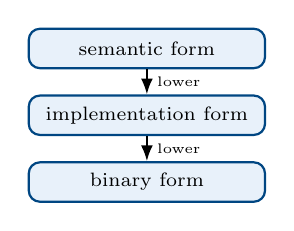
\begin{tikzpicture}[node distance=0.32cm, every node/.style={transform shape},
        box/.style={rectangle,rounded corners,draw=ieeeblue,fill=ieeelight,thick,
          minimum width=3.0cm,minimum height=0.5cm,align=center,font=\scriptsize},
        arrow/.style={-{Latex[length=2mm]},thick}]
        \node[box] (a) {semantic form};
        \node[box,below=of a] (b) {implementation form};
        \node[box,below=of b] (c) {binary form};
        \draw[arrow] (a) -- node[right,font=\tiny]{lower} (b);
        \draw[arrow] (b) -- node[right,font=\tiny]{lower} (c);
      \end{tikzpicture}
    \end{column}
    \begin{column}{0.49\textwidth}
      \begin{block}{Lowered}
        Rewritten closer to the machine while preserving behavior.
      \end{block}
      \begin{itemize}
        \item Conv becomes runtime setup/calls.
        \item Constants become global symbols.
        \item Runtime calls become RV64 calls.
        \item Gemmini helpers become custom instructions.
      \end{itemize}
    \end{column}
  \end{columns}
\end{frame}

% 11
\begin{frame}{Runtime Bridges Generated Code to Hardware}
  \begin{columns}[T]
    \begin{column}{0.54\textwidth}
      \centering
      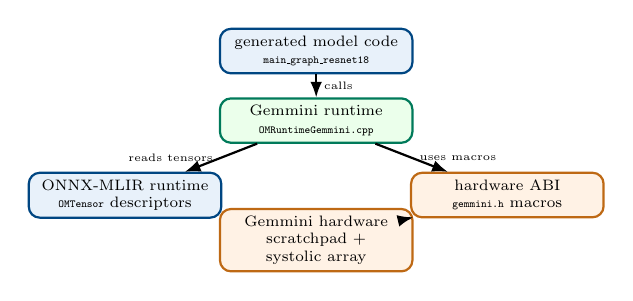
\begin{tikzpicture}[scale=0.78,node distance=0.38cm, every node/.style={transform shape},
        box/.style={rectangle,rounded corners,draw=ieeeblue,fill=ieeelight,thick,
          text width=2.9cm,minimum height=0.62cm,align=center,font=\scriptsize},
        gem/.style={rectangle,rounded corners,draw=stagegreen,fill=green!8,thick,
          text width=2.9cm,minimum height=0.62cm,align=center,font=\scriptsize},
        abibox/.style={rectangle,rounded corners,draw=stageorange,fill=orange!10,thick,
          text width=2.9cm,minimum height=0.62cm,align=center,font=\scriptsize},
        arrow/.style={-{Latex[length=2mm]},thick}]
        \node[box] (model) {generated model code\\\tinycode{main\_graph\_resnet18}};
        \node[gem,below=of model] (runtime) {Gemmini runtime\\\tinycode{OMRuntimeGemmini.cpp}};
        \node[box,below left=0.46cm and -0.05cm of runtime] (tensor) {ONNX-MLIR runtime\\\tinycode{OMTensor} descriptors};
        \node[abibox,below right=0.46cm and -0.05cm of runtime] (abiNode) {hardware ABI\\\tinycode{gemmini.h} macros};
        \node[abibox,below=1.05cm of runtime] (hw) {Gemmini hardware\\scratchpad + systolic array};
        \draw[arrow] (model) -- node[right,font=\tiny] {calls} (runtime);
        \draw[arrow] (runtime) -- node[left,font=\tiny] {reads tensors} (tensor);
        \draw[arrow] (runtime) -- node[right,font=\tiny] {uses macros} (abiNode);
        \draw[arrow] (abiNode) -- (hw);
      \end{tikzpicture}
    \end{column}
    \begin{column}{0.43\textwidth}
      \begin{block}{Runtime}
        Linked support code that executes between generated model code and low-level hardware access.
      \end{block}
      \begin{itemize}
        \item Gives generated code stable C functions to call.
        \item Interprets \code{OMTensor} metadata.
        \item Chooses Gemmini helper kernels and data movement.
        \item Crosses into \code{gemmini.h} for custom instructions.
      \end{itemize}
      \withoutit{generated model code would have to program tensor layouts and Gemmini instructions directly. That would duplicate low-level logic and make the final executable fragile.}
    \end{column}
  \end{columns}
\end{frame}

% 11a
\begin{frame}{How Runtime Moves Tensor Data}
  \centering
  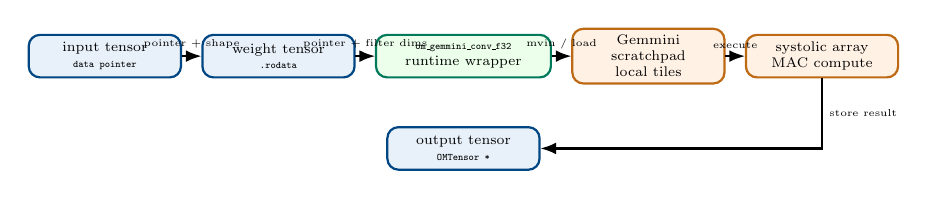
\begin{tikzpicture}[
    scale=0.72,
    every node/.style={transform shape},
    node distance=0.35cm,
    data/.style={rectangle,rounded corners,draw=ieeeblue,fill=ieeelight,thick,
      text width=2.45cm,minimum height=0.75cm,align=center,font=\scriptsize},
    rt/.style={rectangle,rounded corners,draw=stagegreen,fill=green!8,thick,
      text width=2.85cm,minimum height=0.75cm,align=center,font=\scriptsize},
    hw/.style={rectangle,rounded corners,draw=stageorange,fill=orange!10,thick,
      text width=2.45cm,minimum height=0.75cm,align=center,font=\scriptsize},
    arrow/.style={-{Latex[length=2mm]},thick}
  ]
    \node[data] (input) {input tensor\\\tinycode{data pointer}};
    \node[data,right=of input] (weight) {weight tensor\\\tinycode{.rodata}};
    \node[rt,right=of weight] (conv) {\tinycode{om\_gemmini\_conv\_f32}\\runtime wrapper};
    \node[hw,right=of conv] (scratch) {Gemmini scratchpad\\local tiles};
    \node[hw,right=of scratch] (array) {systolic array\\MAC compute};
    \node[data,below=0.85cm of conv] (output) {output tensor\\\tinycode{OMTensor *}};

    \draw[arrow] (input) -- node[above,font=\tiny] {pointer + shape} (weight);
    \draw[arrow] (weight) -- node[above,font=\tiny] {pointer + filter dims} (conv);
    \draw[arrow] (conv) -- node[above,font=\tiny] {mvin / load} (scratch);
    \draw[arrow] (scratch) -- node[above,font=\tiny] {execute} (array);
    \draw[arrow] (array) |- node[pos=0.25,right,font=\tiny] {store result} (output);
  \end{tikzpicture}

  \vspace{0.4em}
  \begin{block}{Meaning}
    Runtime is the active bridge: it reads tensor descriptors, moves tiles to Gemmini-local memory, starts compute, and writes the result back into the output descriptor.
  \end{block}
\end{frame}

% 11b
\begin{frame}{OMTensor Describes One Tensor}
  \begin{columns}
    \begin{column}{0.48\textwidth}
      \centering
      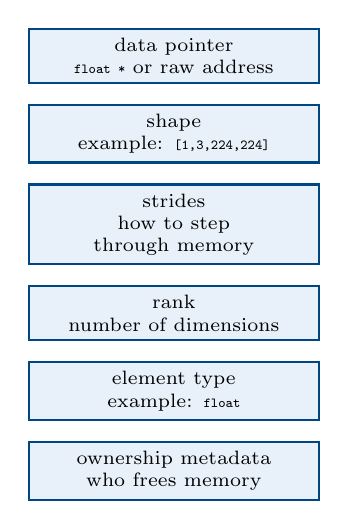
\begin{tikzpicture}[node distance=0.25cm, every node/.style={transform shape},
        field/.style={rectangle,draw=ieeeblue,fill=ieeelight,thick,
          text width=3.45cm,minimum height=0.48cm,align=center,font=\scriptsize}]
        \node[field] (d) {data pointer\\\tinycode{float *} or raw address};
        \node[field,below=of d] (shape) {shape\\example: \tinycode{[1,3,224,224]}};
        \node[field,below=of shape] (strides) {strides\\how to step through memory};
        \node[field,below=of strides] (rank) {rank\\number of dimensions};
        \node[field,below=of rank] (etype) {element type\\example: \tinycode{float}};
        \node[field,below=of etype] (own) {ownership metadata\\who frees memory};
      \end{tikzpicture}
    \end{column}
    \begin{column}{0.49\textwidth}
      \begin{block}{ONNX-MLIR Tensor Descriptor}
        \code{OMTensor} is not the tensor data itself. It is a descriptor that tells runtime code where the data is and how to interpret it.
      \end{block}
      \begin{itemize}
        \item Input image: descriptor points to input floats.
        \item Weight tensor: descriptor points to constant weight memory.
        \item Output tensor: descriptor points to output memory.
        \item Gemmini runtime reads pointer, shape, rank, and type.
      \end{itemize}
      \withoutit{runtime would receive only raw addresses. It would not know shape, rank, element type, strides, or ownership, so convolution dimensions and memory access could be wrong.}
    \end{column}
  \end{columns}
\end{frame}

% 11c
\begin{frame}{How Conv Receives OMTensor Descriptors}
  \centering
  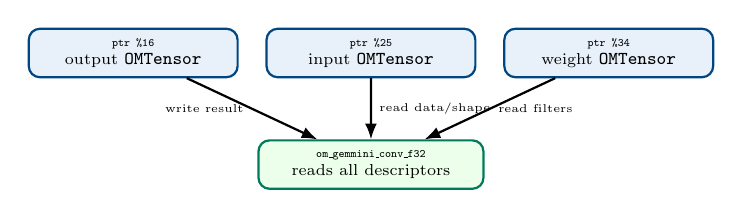
\begin{tikzpicture}[
    scale=0.82,
    every node/.style={transform shape},
    node distance=0.42cm,
    tensor/.style={rectangle,rounded corners,draw=ieeeblue,fill=ieeelight,thick,
      text width=3.0cm,minimum height=0.75cm,align=center,font=\scriptsize},
    rt/.style={rectangle,rounded corners,draw=stagegreen,fill=green!8,thick,
      text width=3.25cm,minimum height=0.75cm,align=center,font=\scriptsize},
    arrow/.style={-{Latex[length=2mm]},thick}
  ]
    \node[tensor] (out) {\tinycode{ptr \%16}\\output \code{OMTensor}};
    \node[tensor,right=of out] (input) {\tinycode{ptr \%25}\\input \code{OMTensor}};
    \node[tensor,right=of input] (weight) {\tinycode{ptr \%34}\\weight \code{OMTensor}};
    \node[rt,below=0.95cm of input] (runtime) {\tinycode{om\_gemmini\_conv\_f32}\\reads all descriptors};

    \draw[arrow] (out) -- node[left,font=\tiny] {write result} (runtime);
    \draw[arrow] (input) -- node[right,font=\tiny] {read data/shape} (runtime);
    \draw[arrow] (weight) -- node[right,font=\tiny] {read filters} (runtime);
  \end{tikzpicture}

  \vspace{0.4em}
  \begin{block}{Concrete Meaning}
    The LLVM call passes addresses of descriptors. The runtime follows each descriptor to find the real tensor memory and dimensions.
  \end{block}
\end{frame}

% 11d
\begin{frame}{OMTensorList Groups Model Inputs and Outputs}
  \begin{columns}
    \begin{column}{0.5\textwidth}
      \centering
      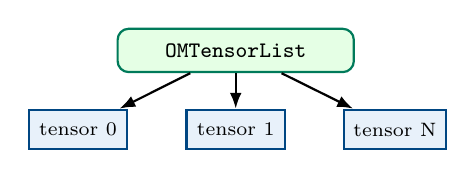
\begin{tikzpicture}[node distance=0.35cm, every node/.style={transform shape},
        list/.style={rectangle,rounded corners,draw=stagegreen,fill=green!10,thick,
          minimum width=3.0cm,minimum height=0.55cm,align=center,font=\scriptsize},
        tensor/.style={rectangle,draw=ieeeblue,fill=ieeelight,thick,
          minimum width=1.25cm,minimum height=0.5cm,align=center,font=\scriptsize},
        arrow/.style={-{Latex[length=2mm]},thick}]
        \node[list] (lst) {\code{OMTensorList}};
        \node[tensor,below left=0.45cm and -0.15cm of lst] (a) {tensor 0};
        \node[tensor,below=0.45cm of lst] (b) {tensor 1};
        \node[tensor,below right=0.45cm and -0.15cm of lst] (c) {tensor N};
        \draw[arrow] (lst) -- (a);
        \draw[arrow] (lst) -- (b);
        \draw[arrow] (lst) -- (c);
      \end{tikzpicture}
    \end{column}
    \begin{column}{0.47\textwidth}
      \begin{block}{Input/Output Container}
        \code{OMTensorList} is the container used at model entry and model return.
      \end{block}
      \begin{itemize}
        \item Input list: one entry per model input.
        \item Output list: one entry per model output.
        \item Each entry is an \code{OMTensor *}.
        \item The graph function unpacks inputs and repacks outputs.
      \end{itemize}
      \withoutit{model entry and return would have no standard container for multiple tensors. Callers could pass inputs in the wrong order or lose output descriptors.}
    \end{column}
  \end{columns}
\end{frame}

% 11e
\begin{frame}{Types Used in This Pipeline}
  \scriptsize
  \begin{tabularx}{\textwidth}{@{}lX@{}}
    \toprule
    Type term & Concrete meaning in this project \\
    \midrule
    \code{float} & 32-bit floating-point number. ResNet weights and activations use this in the float test case. \\
    \code{i64} & 64-bit integer in LLVM IR. Used for values such as stride, padding, sizes, and dimensions. \\
    \code{ptr} & LLVM IR pointer type. In the Conv call it points to an \code{OMTensor} descriptor. \\
    \code{OMTensor *} & C/C++ pointer to one ONNX-MLIR tensor descriptor. Runtime uses it to find data and shape. \\
    \code{OMTensorList *} & Pointer to a container holding multiple \code{OMTensor *} entries for model inputs or outputs. \\
    \code{AnyType} & TableGen/MLIR placeholder meaning the operation accepts a broad MLIR type; later passes verify the real tensor type. \\
    \bottomrule
  \end{tabularx}
\end{frame}

% 12
\begin{frame}{What Is a .td File?}
  \begin{columns}
    \begin{column}{0.5\textwidth}
      \centering
      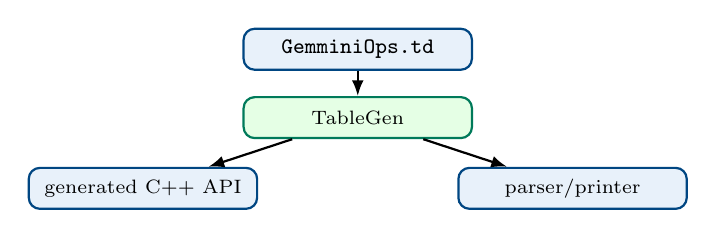
\begin{tikzpicture}[node distance=0.32cm, every node/.style={transform shape},
        box/.style={rectangle,rounded corners,draw=ieeeblue,fill=ieeelight,thick,
          minimum width=2.9cm,minimum height=0.52cm,align=center,font=\scriptsize},
        tool/.style={rectangle,rounded corners,draw=stagegreen,fill=green!10,thick,
          minimum width=2.9cm,minimum height=0.52cm,align=center,font=\scriptsize},
        arrow/.style={-{Latex[length=2mm]},thick}]
        \node[box] (td) {\code{GemminiOps.td}};
        \node[tool,below=of td] (tg) {TableGen};
        \node[box,below left=0.35cm and -0.2cm of tg] (h) {generated C++ API};
        \node[box,below right=0.35cm and -0.2cm of tg] (p) {parser/printer};
        \draw[arrow] (td) -- (tg);
        \draw[arrow] (tg) -- (h);
        \draw[arrow] (tg) -- (p);
      \end{tikzpicture}
    \end{column}
    \begin{column}{0.47\textwidth}
      \begin{block}{TableGen Definition}
        Declarative source for MLIR operations and dialect metadata.
      \end{block}
      \begin{itemize}
        \item Defines operands/results/traits.
        \item Generates C++ declarations.
        \item C++ files implement custom behavior.
      \end{itemize}
    \end{column}
  \end{columns}
\end{frame}

% 13
\begin{frame}[fragile]{TableGen Example: Concept}
  \begin{lstlisting}
// Conceptual shape of a TableGen operation definition.
def Gemmini_ConvOp : Gemmini_Op<"conv", [...]> {
  let arguments = (ins AnyType:$input, AnyType:$weight);
  let results   = (outs AnyType:$output);
  let summary   = "High-level Gemmini convolution";
}
  \end{lstlisting}
  \begin{itemize}
    \item The \code{def} declares an operation.
    \item The operation belongs to a dialect.
    \item \code{AnyType} means TableGen allows a broad MLIR operand type here; verification/lowering decides the concrete tensor type later.
    \item Arguments, results, and attributes become part of the generated C++ API.
  \end{itemize}
\end{frame}

% 14
\sectiondivider{Source Tree Map}{Connect each folder to its compiler responsibility before looking at individual files.}

\begin{frame}{How the Repository Is Organized}
  \scriptsize
  \begin{tabularx}{\textwidth}{@{}lX@{}}
    \toprule
    Folder & Meaning \\
    \midrule
    \code{src/} & Main compiler, dialect, accelerator, runtime, and support source. \\
    \code{include/} & Public project headers. \\
    \code{docs/} & Documentation and generated presentation material. \\
    \code{test/} & ONNX-MLIR compiler and runtime tests. \\
    \code{gemmini/} & Gemmini examples, scripts, tests, and generated artifacts. \\
    \code{gemmini\_toolchain\_build/} & Local build tree for the Gemmini-enabled compiler. \\
    \code{third\_party/} & External dependencies managed separately from project source. \\
    \bottomrule
  \end{tabularx}
\end{frame}

% 15
\begin{frame}{Why We Need a Backend Folder Map}
  \begin{columns}
    \begin{column}{0.48\textwidth}
      \begin{block}{What ``Backend'' Means Here}
        A backend is the part of the compiler that turns a general model representation into code for a specific execution target.
      \end{block}
      \begin{itemize}
        \item Front-end: reads ONNX and creates MLIR operations.
        \item Middle-end: optimizes and rewrites operations.
        \item Backend: chooses Gemmini or fallback paths, lowers operations, emits runtime calls, and prepares target-specific code.
      \end{itemize}
    \end{column}
    \begin{column}{0.48\textwidth}
      \begin{block}{What ``Folder Map'' Means}
        A folder map is a guide that connects source directories to their compiler responsibility.
      \end{block}
      \begin{itemize}
        \item It is not only a file tree.
        \item It explains where each stage of the pipeline lives.
        \item It helps trace a feature from pass registration to lowering, runtime, ABI, and tests.
      \end{itemize}
    \end{column}
  \end{columns}
  \vspace{0.5em}
  \pathcode{src/Accelerators/Gemmini/}
\end{frame}

% 15b
\begin{frame}{How the Gemmini Backend Is Organized}
  \centering
  \vspace*{-0.2em}
  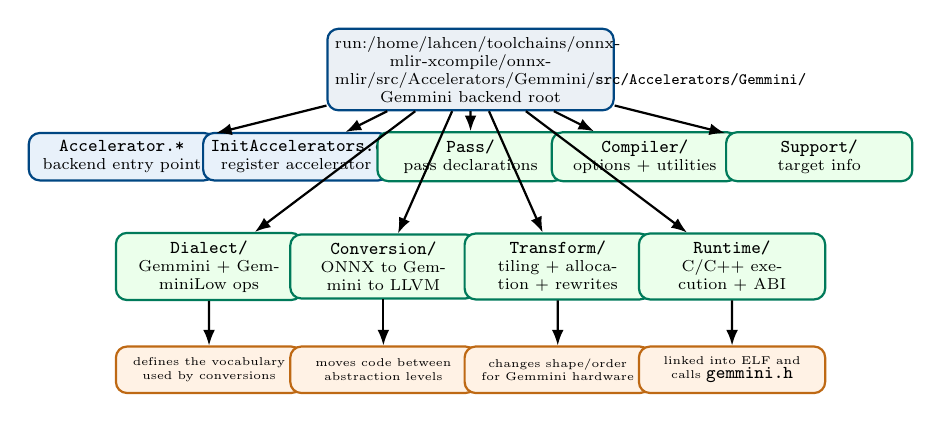
\begin{tikzpicture}[
    scale=0.82,
    every node/.style={transform shape},
    root/.style={rectangle,rounded corners,draw=ieeeblue,fill=ieeeblue!8,thick,
      text width=4.2cm,minimum height=0.7cm,align=center,font=\scriptsize},
    folder/.style={rectangle,rounded corners,draw=stagegreen,fill=green!8,thick,
      text width=2.65cm,minimum height=0.72cm,align=center,font=\scriptsize},
    file/.style={rectangle,rounded corners,draw=ieeeblue,fill=ieeelight,thick,
      text width=2.65cm,minimum height=0.72cm,align=center,font=\scriptsize},
    note/.style={rectangle,rounded corners,draw=stageorange,fill=orange!10,thick,
      text width=2.65cm,minimum height=0.72cm,align=center,font=\tiny},
    arrow/.style={-{Latex[length=2mm]},thick}
  ]
    \node[root] (root) at (0,0) {\pathcode{src/Accelerators/Gemmini/}\\Gemmini backend root};

    \node[file] (entry) at (-5.4,-1.35) {\code{Accelerator.*}\\backend entry point};
    \node[file] (init) at (-2.7,-1.35) {\code{InitAccelerators.cpp}\\register accelerator};
    \node[folder] (pass) at (0,-1.35) {\code{Pass/}\\pass declarations};
    \node[folder] (compiler) at (2.7,-1.35) {\code{Compiler/}\\options + utilities};
    \node[folder] (support) at (5.4,-1.35) {\code{Support/}\\target info};

    \node[folder] (dialect) at (-4.05,-3.05) {\code{Dialect/}\\Gemmini + GemminiLow ops};
    \node[folder] (conversion) at (-1.35,-3.05) {\code{Conversion/}\\ONNX to Gemmini to LLVM};
    \node[folder] (transform) at (1.35,-3.05) {\code{Transform/}\\tiling + allocation + rewrites};
    \node[folder] (runtime) at (4.05,-3.05) {\code{Runtime/}\\C/C++ execution + ABI};

    \node[note] (frontend) at (-4.05,-4.65) {defines the vocabulary\\used by conversions};
    \node[note] (middle) at (-1.35,-4.65) {moves code between\\abstraction levels};
    \node[note] (opt) at (1.35,-4.65) {changes shape/order\\for Gemmini hardware};
    \node[note] (rtNote) at (4.05,-4.65) {linked into ELF and\\calls \code{gemmini.h}};

    \foreach \x in {entry,init,pass,compiler,support,dialect,conversion,transform,runtime}
      \draw[arrow] (root) -- (\x);
    \draw[arrow] (dialect) -- (frontend);
    \draw[arrow] (conversion) -- (middle);
    \draw[arrow] (transform) -- (opt);
    \draw[arrow] (runtime) -- (rtNote);
  \end{tikzpicture}
  \vfill
  \begin{minipage}{0.94\textwidth}
    {\tiny\color{codegray}
    Read this map as responsibilities: registration and options at the top,
    compiler IR vocabulary and lowering in the middle, and runtime/ABI code at the hardware boundary.}
  \end{minipage}
\end{frame}

% 15c
\begin{frame}{What the Backend Root Owns}
  \scriptsize
  \begin{tabularx}{\textwidth}{@{}lX@{}}
    \toprule
    Path & Responsibility \\
    \midrule
    \pathcode{src/Accelerators/Gemmini/} &
      Backend root: owns Gemmini compiler integration, dialects, conversions, transforms, runtime, target info, and pass declarations. \\
    \code{Accelerator.cpp/.hpp} &
      Entry point that lets ONNX-MLIR recognize Gemmini as an accelerator backend. \\
    \code{InitAccelerators.cpp} &
      Registration hook that makes Gemmini available to the accelerator registry. \\
    \pathcode{src/Accelerators/Gemmini/.docs/} &
      Local notes/documentation for the Gemmini backend implementation. \\
    \pathcode{src/Accelerators/Gemmini/Pass/} &
      Public pass declarations. Other compiler code includes these APIs to create and schedule Gemmini passes. \\
    \bottomrule
  \end{tabularx}
\end{frame}

% 15d
\begin{frame}{What Each Backend Subfolder Owns}
  \scriptsize
  \begin{tabularx}{\textwidth}{@{}lX@{}}
    \toprule
    Folder & What It Owns \\
    \midrule
    \pathcode{src/Accelerators/Gemmini/Compiler/} &
      Compiler options and utilities: turns user flags into a concrete Gemmini pass pipeline. \\
    \pathcode{src/Accelerators/Gemmini/Dialect/} &
      MLIR operation vocabulary: defines high-level \code{gemmini} operations and lower-level \code{gemminilow} operations. \\
    \pathcode{src/Accelerators/Gemmini/Conversion/} &
      Lowering between dialects: ONNX to Gemmini, Gemmini to GemminiLow, and GemminiLow to LLVM. \\
    \pathcode{src/Accelerators/Gemmini/Transform/} &
      Optimization and hardware fitting: tiling, static scratchpad allocation, and low-level rewrites. \\
    \pathcode{src/Accelerators/Gemmini/Runtime/} &
      Code linked into the final executable: C/C++ runtime functions plus Gemmini hardware ABI headers. \\
    \pathcode{src/Accelerators/Gemmini/Support/} &
      Target metadata: generated Gemmini hardware parameters used by compiler decisions. \\
    \bottomrule
  \end{tabularx}
\end{frame}

% 15a
\begin{frame}{How to Read Folder Graphs}
  \centering
  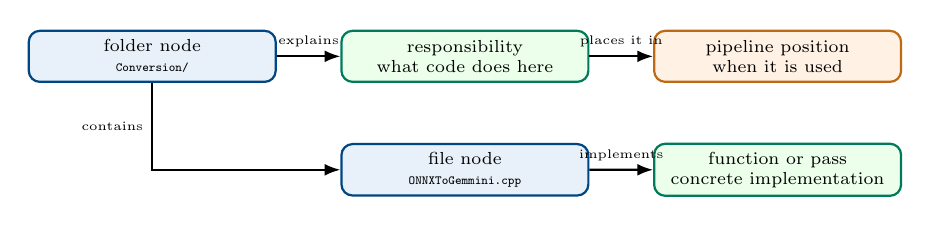
\begin{tikzpicture}[
    scale=0.9,
    every node/.style={transform shape},
    box/.style={rectangle,rounded corners,draw=ieeeblue,fill=ieeelight,thick,
      text width=3.25cm,minimum height=0.72cm,align=center,font=\scriptsize},
    green/.style={rectangle,rounded corners,draw=stagegreen,fill=green!8,thick,
      text width=3.25cm,minimum height=0.72cm,align=center,font=\scriptsize},
    orange/.style={rectangle,rounded corners,draw=stageorange,fill=orange!10,thick,
      text width=3.25cm,minimum height=0.72cm,align=center,font=\scriptsize},
    arrow/.style={-{Latex[length=2mm]},thick}
  ]
    \node[box] (folder) {folder node\\\tinycode{Conversion/}};
    \node[green,right=0.9cm of folder] (meaning) {responsibility\\what code does here};
    \node[orange,right=0.9cm of meaning] (flow) {pipeline position\\when it is used};
    \node[box,below=0.85cm of meaning] (file) {file node\\\tinycode{ONNXToGemmini.cpp}};
    \node[green,right=0.9cm of file] (func) {function or pass\\concrete implementation};

    \draw[arrow] (folder) -- node[above,font=\tiny] {explains} (meaning);
    \draw[arrow] (meaning) -- node[above,font=\tiny] {places it in} (flow);
    \draw[arrow] (folder) |- node[pos=0.25,left,font=\tiny] {contains} (file);
    \draw[arrow] (file) -- node[above,font=\tiny] {implements} (func);
  \end{tikzpicture}

  \vspace{0.5em}
  \begin{block}{Tree Graph Rule}
    Each branch answers one question: where is the code, what responsibility does it own, and when does it participate in the ONNX-to-RV64 pipeline.
  \end{block}
\end{frame}

% 16
\begin{frame}{Compiler Folder Connects Options to Passes}
  \begin{block}{Location}
    \pathcode{src/Accelerators/Gemmini/Compiler/}
  \end{block}
  \begin{itemize}
    \item \code{GemminiCompilerOptions.hpp}: user-facing compiler flags and options.
    \item \code{GemminiCompilerUtils.cpp}: pass-pipeline utility logic.
    \item \code{GemminiCompilerUtils.hpp}: declarations for Gemmini pipeline setup.
  \end{itemize}
  \begin{block}{Purpose}
    This folder connects command-line or build-time Gemmini options to the actual compiler pass pipeline.\\
    It decides which Gemmini-specific passes should be added when the accelerator is enabled.\\
    It keeps pipeline setup code separate from the implementation of each conversion or transform pass.\\
    It gives the compiler one organized place to prepare ONNX-to-Gemmini lowering before code generation.
  \end{block}
\end{frame}

\begin{frame}{How Compiler Files Build the Pass Pipeline}
  \centering
  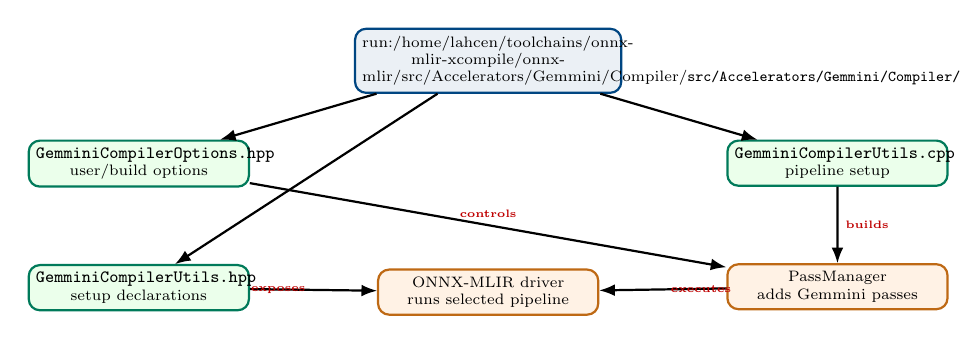
\begin{tikzpicture}[
    scale=0.78,
    every node/.style={transform shape},
    root/.style={rectangle,rounded corners,draw=ieeeblue,fill=ieeeblue!8,thick,
      text width=4.1cm,minimum height=0.68cm,align=center,font=\scriptsize},
    file/.style={rectangle,rounded corners,draw=stagegreen,fill=green!8,thick,
      text width=3.35cm,minimum height=0.72cm,align=center,font=\scriptsize},
    action/.style={rectangle,rounded corners,draw=stageorange,fill=orange!10,thick,
      text width=3.35cm,minimum height=0.72cm,align=center,font=\scriptsize},
    arrow/.style={-{Latex[length=2mm]},thick}
  ]
    \node[root] (root) {\pathcode{src/Accelerators/Gemmini/Compiler/}};
    \node[file,below left=0.75cm and 1.7cm of root] (opts) {\code{GemminiCompilerOptions.hpp}\\user/build options};
    \node[file,below right=0.75cm and 1.7cm of root] (utils) {\code{GemminiCompilerUtils.cpp}\\pipeline setup};
    \node[file,below=1.25cm of opts] (decls) {\code{GemminiCompilerUtils.hpp}\\setup declarations};
    \node[action,below=1.25cm of utils] (pm) {PassManager\\adds Gemmini passes};
    \node[action,below=2.85cm of root] (flow) {ONNX-MLIR driver\\runs selected pipeline};

    \draw[arrow] (root) -- (opts);
    \draw[arrow] (root) -- (utils);
    \draw[arrow] (root) -- (decls);
    \draw[arrow] (opts) -- node[above,font=\tiny] {\edgeword{controls}} (pm);
    \draw[arrow] (utils) -- node[right,font=\tiny] {\edgeword{builds}} (pm);
    \draw[arrow] (decls) -- node[left,font=\tiny] {\edgeword{exposes}} (flow);
    \draw[arrow] (pm) -- node[right,font=\tiny] {\edgeword{executes}} (flow);
  \end{tikzpicture}
  \vspace{0.25em}
  \begin{minipage}{0.94\textwidth}
    {\tiny\color{codegray}
    \edgeword{controls}: options decide which passes are enabled.
    \edgeword{builds}: utility code assembles the pass pipeline.
    \edgeword{exposes}: header gives other code callable declarations.
    \edgeword{executes}: driver runs the selected pass sequence.}
  \end{minipage}
\end{frame}

% 17
\begin{frame}{Conversion Folder Moves Between Dialects}
  \begin{block}{Location}
    \pathcode{src/Accelerators/Gemmini/Conversion/}
  \end{block}
  \begin{itemize}
    \item \code{ONNXToGemmini/}: finds supported ONNX operations and maps them to Gemmini.
    \item \code{GemminiToGemminiLow/}: expands high-level Gemmini intent into lower-level hardware steps.
    \item \code{GemminiLowToLLVM/}: emits LLVM-level calls or inline assembly.
  \end{itemize}
  \begin{block}{Purpose}
    This folder moves the model from high-level graph operations toward executable target code.\\
    It decides when an ONNX operation can become a Gemmini accelerator operation.\\
    It lowers abstract accelerator intent into explicit hardware-oriented load, execute, config, and store steps.\\
    It finally prepares those low-level operations for LLVM and the RISC-V backend.
  \end{block}
\end{frame}

\begin{frame}{How Conversion Files Lower the Model}
  \centering
  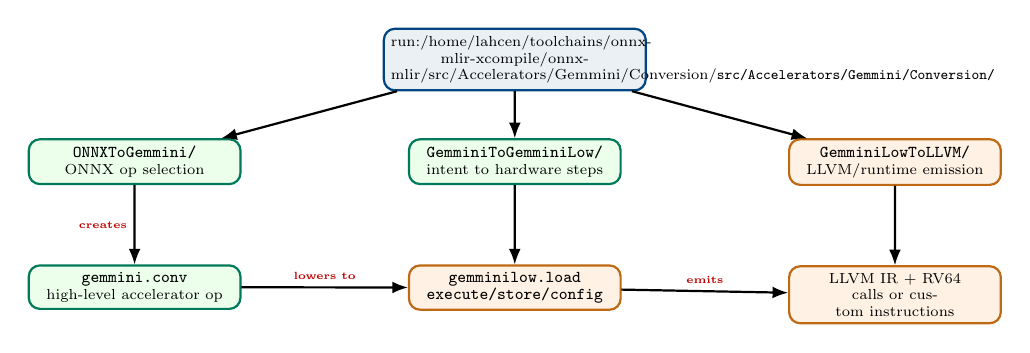
\begin{tikzpicture}[
    scale=0.75,
    every node/.style={transform shape},
    root/.style={rectangle,rounded corners,draw=ieeeblue,fill=ieeeblue!8,thick,
      text width=4.2cm,minimum height=0.68cm,align=center,font=\scriptsize},
    stage/.style={rectangle,rounded corners,draw=stagegreen,fill=green!8,thick,
      text width=3.35cm,minimum height=0.72cm,align=center,font=\scriptsize},
    low/.style={rectangle,rounded corners,draw=stageorange,fill=orange!10,thick,
      text width=3.35cm,minimum height=0.72cm,align=center,font=\scriptsize},
    arrow/.style={-{Latex[length=2mm]},thick}
  ]
    \node[root] (root) {\pathcode{src/Accelerators/Gemmini/Conversion/}};
    \node[stage,below left=0.8cm and 2.4cm of root] (onnx) {\code{ONNXToGemmini/}\\ONNX op selection};
    \node[stage,below=0.8cm of root] (mid) {\code{GemminiToGemminiLow/}\\intent to hardware steps};
    \node[low,below right=0.8cm and 2.4cm of root] (llvm) {\code{GemminiLowToLLVM/}\\LLVM/runtime emission};
    \node[stage,below=1.35cm of onnx] (gemmini) {\code{gemmini.conv}\\high-level accelerator op};
    \node[low,below=1.35cm of mid] (gemlow) {\code{gemminilow.load}\\\code{execute/store/config}};
    \node[low,below=1.35cm of llvm] (rv) {LLVM IR + RV64\\calls or custom instructions};

    \draw[arrow] (root) -- (onnx);
    \draw[arrow] (root) -- (mid);
    \draw[arrow] (root) -- (llvm);
    \draw[arrow] (onnx) -- node[left,font=\tiny] {\edgeword{creates}} (gemmini);
    \draw[arrow] (gemmini) -- node[above,font=\tiny] {\edgeword{lowers to}} (gemlow);
    \draw[arrow] (mid) -- (gemlow);
    \draw[arrow] (gemlow) -- node[above,font=\tiny] {\edgeword{emits}} (rv);
    \draw[arrow] (llvm) -- (rv);
  \end{tikzpicture}
  \vspace{0.25em}
  \begin{minipage}{0.94\textwidth}
    {\tiny\color{codegray}
    \edgeword{creates}: rewrites an ONNX operation into a Gemmini operation.
    \edgeword{lowers to}: replaces an abstract op with more concrete lower-level steps.
    \edgeword{emits}: produces LLVM/runtime/RV64-facing code from GemminiLow.}
  \end{minipage}
\end{frame}

% 18
\begin{frame}{Dialect Folder Defines Gemmini Vocabulary}
  \begin{block}{Location}
    \pathcode{src/Accelerators/Gemmini/Dialect/}
  \end{block}
  \begin{itemize}
    \item \code{Dialect/Gemmini/}: high-level accelerator operations such as conv and matmul.
    \item \code{Dialect/GemminiLow/}: hardware-near operations such as load, execute, store, and config.
    \item \code{*.td}: declarative operation definitions.
    \item \code{*Ops.cpp}: operation behavior, side effects, folding, verification support.
  \end{itemize}
  \begin{block}{Purpose}
    This folder defines the words that Gemmini passes are allowed to use inside MLIR.\\
    It separates high-level accelerator meaning from hardware-near scheduling details.\\
    It gives conversion and transform passes typed operations instead of loose strings or comments.\\
    It lets MLIR verify, print, parse, and rewrite Gemmini operations in a structured way.
  \end{block}
\end{frame}

\begin{frame}{How Dialect Files Define Operations}
  \centering
  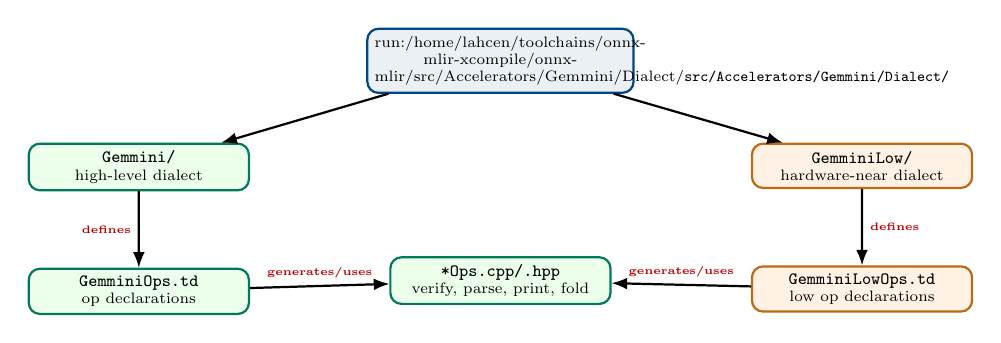
\begin{tikzpicture}[
    scale=0.78,
    every node/.style={transform shape},
    root/.style={rectangle,rounded corners,draw=ieeeblue,fill=ieeeblue!8,thick,
      text width=4.1cm,minimum height=0.68cm,align=center,font=\scriptsize},
    high/.style={rectangle,rounded corners,draw=stagegreen,fill=green!8,thick,
      text width=3.35cm,minimum height=0.72cm,align=center,font=\scriptsize},
    low/.style={rectangle,rounded corners,draw=stageorange,fill=orange!10,thick,
      text width=3.35cm,minimum height=0.72cm,align=center,font=\scriptsize},
    arrow/.style={-{Latex[length=2mm]},thick}
  ]
    \node[root] (root) {\pathcode{src/Accelerators/Gemmini/Dialect/}};
    \node[high,below left=0.8cm and 1.9cm of root] (gemmini) {\code{Gemmini/}\\high-level dialect};
    \node[low,below right=0.8cm and 1.9cm of root] (gemlow) {\code{GemminiLow/}\\hardware-near dialect};
    \node[high,below=1.25cm of gemmini] (td1) {\code{GemminiOps.td}\\op declarations};
    \node[low,below=1.25cm of gemlow] (td2) {\code{GemminiLowOps.td}\\low op declarations};
    \node[high,below=2.65cm of root] (ops) {\code{*Ops.cpp/.hpp}\\verify, parse, print, fold};

    \draw[arrow] (root) -- (gemmini);
    \draw[arrow] (root) -- (gemlow);
    \draw[arrow] (gemmini) -- node[left,font=\tiny] {\edgeword{defines}} (td1);
    \draw[arrow] (gemlow) -- node[right,font=\tiny] {\edgeword{defines}} (td2);
    \draw[arrow] (td1) -- node[above,font=\tiny] {\edgeword{generates/uses}} (ops);
    \draw[arrow] (td2) -- node[above,font=\tiny] {\edgeword{generates/uses}} (ops);
  \end{tikzpicture}
  \vspace{0.25em}
  \begin{minipage}{0.94\textwidth}
    {\tiny\color{codegray}
    \edgeword{defines}: TableGen files declare valid MLIR operations and fields.
    \edgeword{generates/uses}: TableGen creates C++ operation scaffolding, while C++ files add behavior such as verification, parsing, printing, and folding.}
  \end{minipage}
\end{frame}

% 19
\begin{frame}{Transform Folder Fits IR to Hardware}
  \begin{block}{Location}
    \pathcode{src/Accelerators/Gemmini/Transform/}
  \end{block}
  \begin{itemize}
    \item \code{Transform/Gemmini/GemminiTiling.cpp}: high-level tiling.
    \item \code{Transform/GemminiLow/StaticScratchpadAllocation.cpp}: scratchpad address assignment.
    \item \code{Transform/GemminiLow/GemminiLowRewrite.cpp}: low-level cleanup and rewrite patterns.
  \end{itemize}
  \begin{block}{Purpose}
    This folder reshapes the compiler IR so it better matches Gemmini hardware limits.\\
    It tiles large tensors into blocks that can fit in scratchpad and accumulator memory.\\
    It assigns static local-memory locations so later lowering has concrete hardware addresses.\\
    It rewrites low-level operations to reduce ambiguity before LLVM code generation.
  \end{block}
\end{frame}

\begin{frame}{How Transform Files Prepare Hardware-Friendly IR}
  \centering
  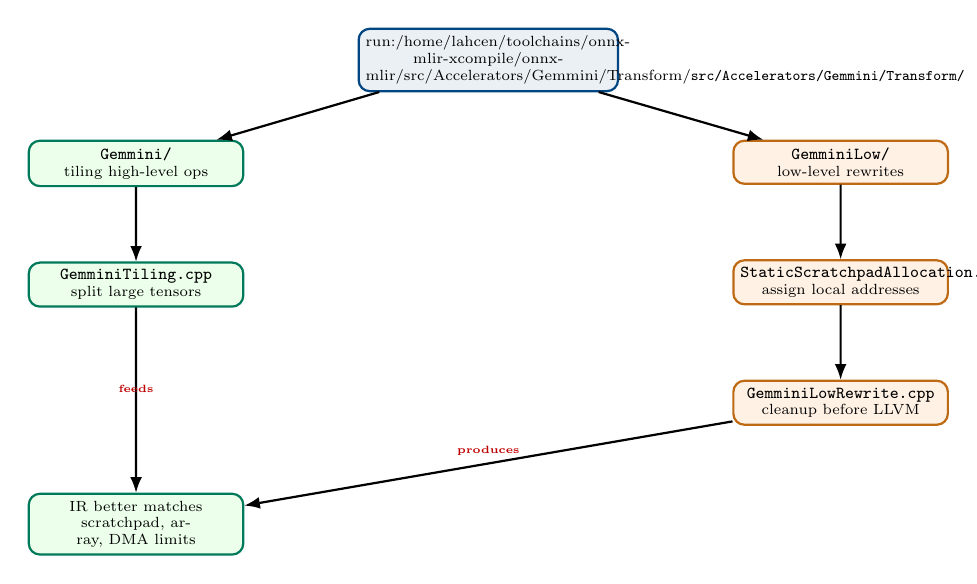
\begin{tikzpicture}[
    scale=0.76,
    every node/.style={transform shape},
    root/.style={rectangle,rounded corners,draw=ieeeblue,fill=ieeeblue!8,thick,
      text width=4.1cm,minimum height=0.68cm,align=center,font=\scriptsize},
    high/.style={rectangle,rounded corners,draw=stagegreen,fill=green!8,thick,
      text width=3.35cm,minimum height=0.72cm,align=center,font=\scriptsize},
    low/.style={rectangle,rounded corners,draw=stageorange,fill=orange!10,thick,
      text width=3.35cm,minimum height=0.72cm,align=center,font=\scriptsize},
    arrow/.style={-{Latex[length=2mm]},thick}
  ]
    \node[root] (root) {\pathcode{src/Accelerators/Gemmini/Transform/}};
    \node[high,below left=0.8cm and 1.9cm of root] (tile) {\code{Gemmini/}\\tiling high-level ops};
    \node[low,below right=0.8cm and 1.9cm of root] (lowdir) {\code{GemminiLow/}\\low-level rewrites};
    \node[high,below=1.25cm of tile] (tilefile) {\code{GemminiTiling.cpp}\\split large tensors};
    \node[low,below=1.25cm of lowdir] (alloc) {\code{StaticScratchpadAllocation.cpp}\\assign local addresses};
    \node[low,below=1.25cm of alloc] (rewrite) {\code{GemminiLowRewrite.cpp}\\cleanup before LLVM};
    \node[high,below=3.1cm of tilefile] (result) {IR better matches\\scratchpad, array, DMA limits};

    \draw[arrow] (root) -- (tile);
    \draw[arrow] (root) -- (lowdir);
    \draw[arrow] (tile) -- (tilefile);
    \draw[arrow] (lowdir) -- (alloc);
    \draw[arrow] (alloc) -- (rewrite);
    \draw[arrow] (tilefile) -- node[above,font=\tiny] {\edgeword{feeds}} (result);
    \draw[arrow] (rewrite) -- node[above,font=\tiny] {\edgeword{produces}} (result);
  \end{tikzpicture}
  \vspace{0.25em}
  \begin{minipage}{0.94\textwidth}
    {\tiny\color{codegray}
    \edgeword{feeds}: high-level tiling output becomes input for later low-level passes.
    \edgeword{produces}: rewrite/allocation passes create IR that is closer to Gemmini hardware limits.}
  \end{minipage}
\end{frame}

% 20
\begin{frame}{Runtime Folder Links Model Code to Gemmini}
  \begin{block}{Location}
    \pathcode{src/Accelerators/Gemmini/Runtime/}
  \end{block}
  \begin{itemize}
    \item \code{OMRuntimeGemmini.hpp}: declarations used by generated or lowered model code.
    \item \code{OMRuntimeGemmini.cpp}: C/C++ implementations linked into the final executable.
    \item \code{gemmini-hardware-abi/include/}: Gemmini macros, parameters, and helper headers.
    \item This folder is where compiler output becomes callable code that can reach the accelerator.
  \end{itemize}
  \begin{block}{Purpose}
    This folder provides the executable software bridge between ONNX-MLIR generated code and Gemmini hardware.\\
    It implements stable runtime functions such as convolution wrappers that the lowered model can call.\\
    It includes the hardware ABI headers that encode Gemmini custom instruction usage and parameters.\\
    It keeps model code, runtime code, and hardware commands connected during final linking and execution.
  \end{block}
\end{frame}

\begin{frame}{How Runtime Files Reach the ABI}
  \centering
  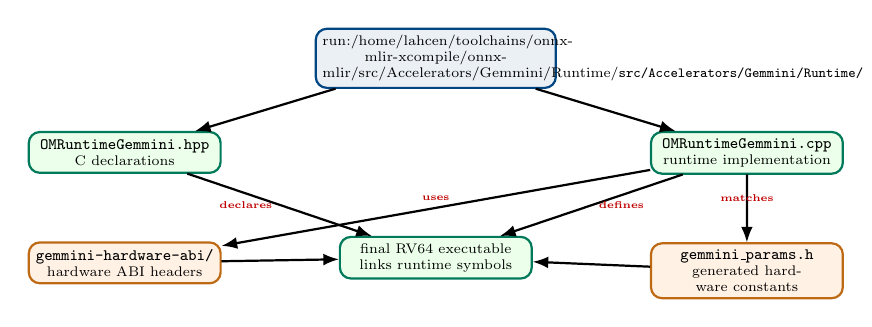
\begin{tikzpicture}[
    scale=0.72,
    every node/.style={transform shape},
    root/.style={rectangle,rounded corners,draw=ieeeblue,fill=ieeeblue!8,thick,
      text width=4.0cm,minimum height=0.68cm,align=center,font=\scriptsize},
    file/.style={rectangle,rounded corners,draw=stagegreen,fill=green!8,thick,
      text width=3.15cm,minimum height=0.72cm,align=center,font=\scriptsize},
    abi/.style={rectangle,rounded corners,draw=stageorange,fill=orange!10,thick,
      text width=3.15cm,minimum height=0.72cm,align=center,font=\scriptsize},
    arrow/.style={-{Latex[length=2mm]},thick}
  ]
    \node[root] (root) {\pathcode{src/Accelerators/Gemmini/Runtime/}};
    \node[file,below left=0.75cm and 1.65cm of root] (hpp) {\code{OMRuntimeGemmini.hpp}\\C declarations};
    \node[file,below right=0.75cm and 1.65cm of root] (cpp) {\code{OMRuntimeGemmini.cpp}\\runtime implementation};
    \node[abi,below=1.2cm of hpp] (abi) {\code{gemmini-hardware-abi/}\\hardware ABI headers};
    \node[abi,below=1.2cm of cpp] (params) {\code{gemmini\_params.h}\\generated hardware constants};
    \node[file,below=2.6cm of root] (elf) {final RV64 executable\\links runtime symbols};

    \draw[arrow] (root) -- (hpp);
    \draw[arrow] (root) -- (cpp);
    \draw[arrow] (hpp) -- node[left,font=\tiny] {\edgeword{declares}} (elf);
    \draw[arrow] (cpp) -- node[right,font=\tiny] {\edgeword{defines}} (elf);
    \draw[arrow] (cpp) -- node[above,font=\tiny] {\edgeword{uses}} (abi);
    \draw[arrow] (cpp) -- node[above,font=\tiny] {\edgeword{matches}} (params);
    \draw[arrow] (abi) -- (elf);
    \draw[arrow] (params) -- (elf);
  \end{tikzpicture}
  \vspace{0.25em}
  \begin{minipage}{0.94\textwidth}
    {\tiny\color{codegray}
    \edgeword{declares}: header publishes runtime function signatures.
    \edgeword{defines}: C++ file implements those functions.
    \edgeword{uses}: runtime calls ABI macros.
    \edgeword{matches}: runtime constants align with generated Gemmini parameters.}
  \end{minipage}
\end{frame}

% 21
\begin{frame}{Support Folder Shares Hardware Facts}
  \begin{block}{Location}
    \pathcode{src/Accelerators/Gemmini/Support/}
  \end{block}
  \begin{itemize}
    \item \code{GemminiTargetInfo.hpp.in}: CMake template generated from \code{gemmini\_params.h}.
    \item \code{GemminiTargetInfo.cpp}: target information implementation.
    \item Important reason: the compiler must know hardware sizes such as mesh dimensions, scratchpad capacity, and data widths before lowering.
    \item Generated information keeps compiler assumptions aligned with the runtime ABI and \code{gemmini\_params.h}.
  \end{itemize}
  \begin{block}{Purpose}
    This folder keeps target-specific hardware facts available to compiler code.\\
    It prevents the compiler from hard-coding a second copy of Gemmini configuration values.\\
    It lets CMake generate target information from the same parameters used by the runtime ABI.\\
    It helps passes make lowering decisions that match the actual configured Gemmini hardware.
  \end{block}
\end{frame}

\begin{frame}{How Support Files Avoid Duplicate Configuration}
  \centering
  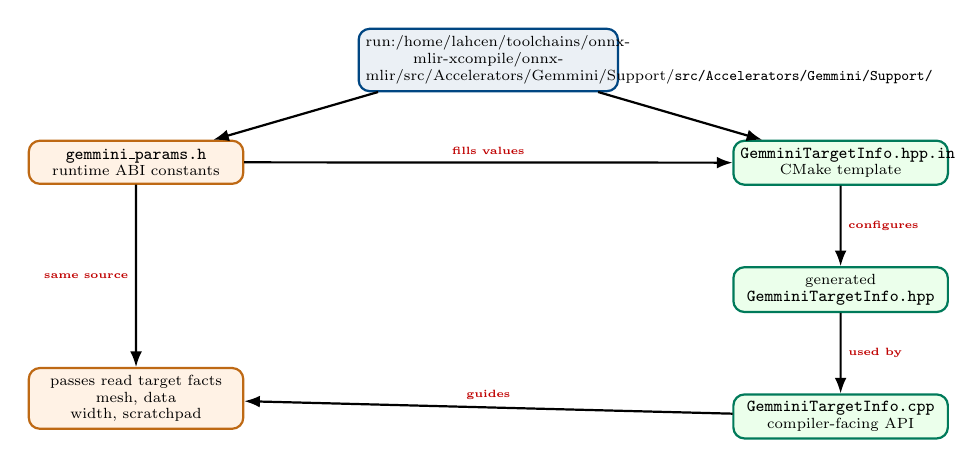
\begin{tikzpicture}[
    scale=0.76,
    every node/.style={transform shape},
    root/.style={rectangle,rounded corners,draw=ieeeblue,fill=ieeeblue!8,thick,
      text width=4.1cm,minimum height=0.68cm,align=center,font=\scriptsize},
    src/.style={rectangle,rounded corners,draw=stageorange,fill=orange!10,thick,
      text width=3.35cm,minimum height=0.72cm,align=center,font=\scriptsize},
    gen/.style={rectangle,rounded corners,draw=stagegreen,fill=green!8,thick,
      text width=3.35cm,minimum height=0.72cm,align=center,font=\scriptsize},
    arrow/.style={-{Latex[length=2mm]},thick}
  ]
    \node[root] (root) {\pathcode{src/Accelerators/Gemmini/Support/}};
    \node[src,below left=0.8cm and 1.9cm of root] (params) {\code{gemmini\_params.h}\\runtime ABI constants};
    \node[gen,below right=0.8cm and 1.9cm of root] (template) {\code{GemminiTargetInfo.hpp.in}\\CMake template};
    \node[gen,below=1.35cm of template] (hpp) {generated\\\code{GemminiTargetInfo.hpp}};
    \node[gen,below=1.35cm of hpp] (cpp) {\code{GemminiTargetInfo.cpp}\\compiler-facing API};
    \node[src,below=3.05cm of params] (passes) {passes read target facts\\mesh, data width, scratchpad};

    \draw[arrow] (root) -- (params);
    \draw[arrow] (root) -- (template);
    \draw[arrow] (params) -- node[above,font=\tiny] {\edgeword{fills values}} (template);
    \draw[arrow] (template) -- node[right,font=\tiny] {\edgeword{configures}} (hpp);
    \draw[arrow] (hpp) -- node[right,font=\tiny] {\edgeword{used by}} (cpp);
    \draw[arrow] (cpp) -- node[above,font=\tiny] {\edgeword{guides}} (passes);
    \draw[arrow] (params) -- node[left,font=\tiny] {\edgeword{same source}} (passes);
  \end{tikzpicture}
  \vspace{0.25em}
  \begin{minipage}{0.94\textwidth}
    {\tiny\color{codegray}
    \edgeword{fills values}: hardware constants are copied into the template.
    \edgeword{configures}: CMake produces the generated target-info header.
    \edgeword{used by}: implementation reads the generated declarations.
    \edgeword{guides}: passes use target facts for lowering decisions.}
  \end{minipage}
\end{frame}

% 21a
\begin{frame}{Pass Folder Exposes Compiler Steps}
  \begin{block}{Location}
    \pathcode{src/Accelerators/Gemmini/Pass/}
  \end{block}
  \begin{itemize}
    \item Main role: declare Gemmini pass creation APIs in one public place.
    \item \code{GemminiPasses.hpp}: exposes pass constructors used by the compiler pipeline.
    \item Pass declarations are not the full implementations; implementations live in \code{Conversion/} and \code{Transform/}.
    \item This folder is the connector between pipeline setup and concrete lowering/optimization code.
    \item Example: a driver can request ``convert ONNX to Gemmini'' without knowing the internal file that implements the rewrite patterns.
  \end{itemize}
  \begin{block}{Purpose}
    This folder gives the rest of ONNX-MLIR a clean way to ask for Gemmini compiler passes.\\
    It exposes pass creation functions without forcing callers to know implementation files.\\
    It keeps the public pass interface separate from conversion and transform internals.\\
    It helps the compiler pipeline schedule Gemmini lowering steps in the correct order.
  \end{block}
\end{frame}

\begin{frame}{How Pass Files Register Lowering Work}
  \centering
  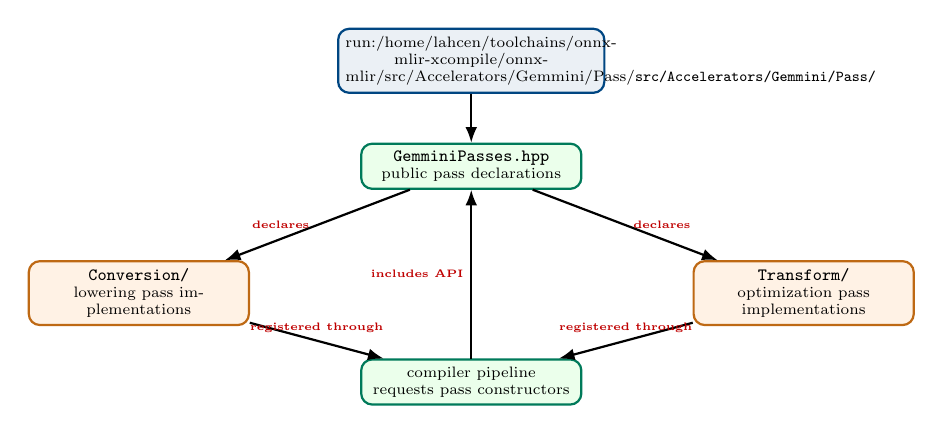
\begin{tikzpicture}[
    scale=0.78,
    every node/.style={transform shape},
    root/.style={rectangle,rounded corners,draw=ieeeblue,fill=ieeeblue!8,thick,
      text width=4.1cm,minimum height=0.68cm,align=center,font=\scriptsize},
    api/.style={rectangle,rounded corners,draw=stagegreen,fill=green!8,thick,
      text width=3.35cm,minimum height=0.72cm,align=center,font=\scriptsize},
    impl/.style={rectangle,rounded corners,draw=stageorange,fill=orange!10,thick,
      text width=3.35cm,minimum height=0.72cm,align=center,font=\scriptsize},
    arrow/.style={-{Latex[length=2mm]},thick}
  ]
    \node[root] (root) {\pathcode{src/Accelerators/Gemmini/Pass/}};
    \node[api,below=0.8cm of root] (hpp) {\code{GemminiPasses.hpp}\\public pass declarations};
    \node[impl,below left=1.15cm and 1.8cm of hpp] (conv) {\code{Conversion/}\\lowering pass implementations};
    \node[impl,below right=1.15cm and 1.8cm of hpp] (trans) {\code{Transform/}\\optimization pass implementations};
    \node[api,below=2.75cm of hpp] (pipeline) {compiler pipeline\\requests pass constructors};

    \draw[arrow] (root) -- (hpp);
    \draw[arrow] (hpp) -- node[left,font=\tiny] {\edgeword{declares}} (conv);
    \draw[arrow] (hpp) -- node[right,font=\tiny] {\edgeword{declares}} (trans);
    \draw[arrow] (pipeline) -- node[left,font=\tiny] {\edgeword{includes API}} (hpp);
    \draw[arrow] (conv) -- node[above,font=\tiny] {\edgeword{registered through}} (pipeline);
    \draw[arrow] (trans) -- node[above,font=\tiny] {\edgeword{registered through}} (pipeline);
  \end{tikzpicture}
  \vspace{0.25em}
  \begin{minipage}{0.94\textwidth}
    {\tiny\color{codegray}
    \edgeword{declares}: public header names pass creation functions.
    \edgeword{includes API}: pipeline code imports those declarations.
    \edgeword{registered through}: concrete conversion/transform passes are made available to the pipeline by this public interface.}
  \end{minipage}
\end{frame}

% 22
\sectiondivider{Compiler Architecture}{Follow the model as compiler passes lower it from ONNX semantics to Gemmini-aware execution.}

\begin{frame}{Use the Real ONNX Folder Layout}
  \begin{block}{Actual Location}
    \pathcode{src/Dialect/ONNX/}
  \end{block}
  \begin{itemize}
    \item The actual tree contains \code{ONNXOps/}, \code{ElementsAttr/}, and \code{Transforms/}.
    \item There is no \code{src/Dialect/ONNX/ShapeInference/} folder in this checkout.
    \item Shape-related logic is organized through ONNX operation implementations, generated code, and transform utilities.
    \item The presentation therefore uses the real folder name: \code{Transforms/}.
  \end{itemize}
\end{frame}

% 23
\begin{frame}{ONNX Stage Preserves Model Semantics}
  \begin{block}{Role}
    Represent the user model in MLIR while preserving ONNX semantics.
  \end{block}
  \begin{itemize}
    \item Input file: \code{model.onnx}.
    \item Important source folder: \pathcode{src/Dialect/ONNX/}.
    \item Main operation definitions: \code{ONNXOps.td} and operation-specific files under \code{ONNXOps/}.
    \item Output: ONNX dialect MLIR that can be transformed by ONNX-MLIR passes.
  \end{itemize}
\end{frame}

% 24
\begin{frame}{ONNX to Gemmini Selects Accelerator Ops}
  \begin{block}{Location}
    \pathcode{src/Accelerators/Gemmini/Conversion/ONNXToGemmini/}
  \end{block}
  \begin{itemize}
    \item Checks whether an ONNX operation is supported by the Gemmini backend.
    \item Converts selected operations such as Conv, MatMul, Gemm, Add, Relu, and pooling.
    \item Keeps unsupported operations available for fallback or other lowering paths.
    \item This is the first accelerator-specific decision point.
  \end{itemize}
\end{frame}

% 25
\begin{frame}{Gemmini Dialect Captures Accelerator Intent}
  \begin{block}{Why it exists}
    The compiler needs a representation that says "this operation should use Gemmini" without committing to every hardware instruction yet.
  \end{block}
  \begin{itemize}
    \item A \code{gemmini.conv} still looks like a convolution.
    \item The operation can carry shape, stride, padding, and dataflow information.
    \item Tiling and legality checks can still operate at a meaningful neural-network level.
    \item This level is easier to reason about than raw DMA and custom instructions.
  \end{itemize}
\end{frame}

% 25b
\begin{frame}{Accelerator Intent Marks Work for Gemmini}
  \begin{columns}
    \begin{column}{0.5\textwidth}
      \centering
      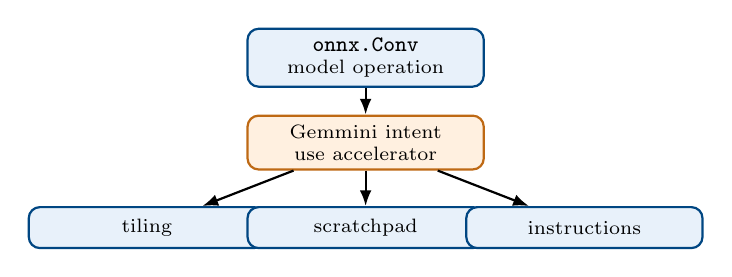
\begin{tikzpicture}[node distance=0.34cm, every node/.style={transform shape},
        box/.style={rectangle,rounded corners,draw=ieeeblue,fill=ieeelight,thick,
          minimum width=3.0cm,minimum height=0.52cm,align=center,font=\scriptsize},
        intent/.style={rectangle,rounded corners,draw=stageorange,fill=orange!12,thick,
          minimum width=3.0cm,minimum height=0.52cm,align=center,font=\scriptsize},
        arrow/.style={-{Latex[length=2mm]},thick}]
        \node[box] (onnx) {\code{onnx.Conv}\\model operation};
        \node[intent,below=of onnx] (intent) {Gemmini intent\\use accelerator};
        \node[box,below left=0.45cm and -0.25cm of intent] (tile) {tiling};
        \node[box,below=0.45cm of intent] (spad) {scratchpad};
        \node[box,below right=0.45cm and -0.25cm of intent] (insn) {instructions};
        \draw[arrow] (onnx) -- (intent);
        \draw[arrow] (intent) -- (tile);
        \draw[arrow] (intent) -- (spad);
        \draw[arrow] (intent) -- (insn);
      \end{tikzpicture}
    \end{column}
    \begin{column}{0.47\textwidth}
      \begin{block}{Accelerator Intent}
        Decision that an operation should use Gemmini before exact hardware steps are chosen.
      \end{block}
      \begin{itemize}
        \item Keeps Conv/MatMul semantics.
        \item Still carries shape, stride, padding.
        \item Later passes choose schedule and instructions.
      \end{itemize}
      \withoutit{the compiler would jump from ONNX directly to raw hardware details. Tiling, legality checks, and accelerator selection would be harder to reason about.}
    \end{column}
  \end{columns}
\end{frame}

% 26
\begin{frame}{GemminiLow Exposes Hardware Steps}
  \begin{block}{Why it exists}
    Gemmini hardware execution is not one abstract operation. It needs configuration, memory transfers, compute commands, and stores.
  \end{block}
  \begin{itemize}
    \item \code{gemminilow.config}: program dataflow, strides, scaling, and mode.
    \item \code{gemminilow.load}: move data into the scratchpad.
    \item \code{gemminilow.execute}: launch systolic-array computation.
    \item \code{gemminilow.store}: move results back to memory.
  \end{itemize}
  \withoutit{one high-level \code{gemmini.conv} would hide the required hardware sequence. The compiler could not schedule loads, compute, stores, or scratchpad use explicitly.}
\end{frame}

% 27
\begin{frame}[fragile]{How Gemmini Becomes GemminiLow}
  \begin{lstlisting}
// High-level intent:
gemmini.conv(input, weight, output, stride=2, pad=3)

// Lower-level execution shape:
gemminilow.config(dataflow, strides, scale)
gemminilow.load(input_tile, scratchpad_A)
gemminilow.load(weight_tile, scratchpad_B)
gemminilow.execute(scratchpad_A, scratchpad_B, accumulator)
gemminilow.store(accumulator, output_tile)
  \end{lstlisting}
  \begin{itemize}
    \item Gemmini is compiler-friendly.
    \item GemminiLow is hardware-scheduling-friendly.
  \end{itemize}
\end{frame}

% 28
\begin{frame}{Tiling Makes Large Tensors Fit}
  \begin{block}{Location}
    \pathcode{src/Accelerators/Gemmini/Transform/Gemmini/GemminiTiling.cpp}
  \end{block}
  \begin{itemize}
    \item Large tensors may not fit directly into accelerator-local storage.
    \item Tiling partitions the work into blocks that match Gemmini array and scratchpad limits.
    \item Tiling exposes reuse: weights or activations can stay in local memory across multiple operations.
    \item The result is a better schedule for later GemminiLow lowering.
  \end{itemize}
  \withoutit{large ResNet tensors may exceed scratchpad or accumulator limits. The runtime would move too much data at once or lose reuse opportunities.}
\end{frame}

% 29
\begin{frame}{Scratchpad Allocation Assigns Local Addresses}
  \begin{block}{Location}
    \pathcode{src/Accelerators/Gemmini/Transform/GemminiLow/StaticScratchpadAllocation.cpp}
  \end{block}
  \begin{itemize}
    \item Gemmini has a scratchpad and accumulator memory separate from normal DRAM.
    \item The compiler must assign addresses for tiles and intermediate results.
    \item Static allocation makes those addresses explicit before LLVM lowering.
    \item This reduces ambiguity when emitting low-level code.
  \end{itemize}
  \withoutit{GemminiLow operations would refer to local memory without stable addresses. Tiles could overlap, overwrite each other, or be loaded from the wrong scratchpad location.}
\end{frame}

% 30
\begin{frame}{GemminiLow to LLVM Emits Runtime/Instruction Hooks}
  \begin{block}{Location}
    \pathcode{src/Accelerators/Gemmini/Conversion/GemminiLowToLLVM/}
  \end{block}
  \begin{itemize}
    \item Converts GemminiLow operations into LLVM-compatible constructs.
    \item Can emit calls to runtime functions.
    \item Can emit inline assembly for RISC-V custom instructions.
    \item The output is ready for LLVM IR generation and RISC-V code generation.
  \end{itemize}
\end{frame}

% 31
\begin{frame}{Hardware ABI Headers Define Gemmini Commands}
  \begin{block}{Location}
    \pathcode{src/Accelerators/Gemmini/Runtime/gemmini-hardware-abi/include/}
  \end{block}
  \begin{itemize}
    \item \code{gemmini.h}: main instruction macros and low-level accelerator interface.
    \item \code{gemmini\_params.h}: generated hardware configuration.
    \item \code{gemmini\_nn.h}: neural-network helper functions.
    \item \code{gemmini\_counter.h}: performance counters.
    \item These files define the contract expected by generated and runtime code.
  \end{itemize}
\end{frame}

% 32
\begin{frame}{Runtime Functions Execute Selected Ops}
  \centering
  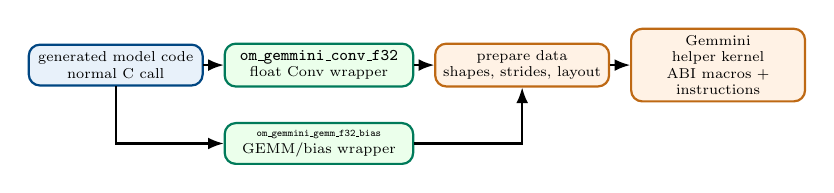
\begin{tikzpicture}[
    scale=0.74,
    every node/.style={transform shape},
    node distance=0.35cm,
    call/.style={rectangle,rounded corners,draw=ieeeblue,fill=ieeelight,thick,
      text width=2.75cm,minimum height=0.7cm,align=center,font=\scriptsize},
    rt/.style={rectangle,rounded corners,draw=stagegreen,fill=green!8,thick,
      text width=3.0cm,minimum height=0.7cm,align=center,font=\scriptsize},
    hw/.style={rectangle,rounded corners,draw=stageorange,fill=orange!10,thick,
      text width=2.75cm,minimum height=0.7cm,align=center,font=\scriptsize},
    arrow/.style={-{Latex[length=2mm]},thick}
  ]
    \node[call] (generated) {generated model code\\normal C call};
    \node[rt,right=of generated] (conv) {\code{om\_gemmini\_conv\_f32}\\float Conv wrapper};
    \node[rt,below=0.6cm of conv] (gemm) {\tinycode{om\_gemmini\_gemm\_f32\_bias}\\GEMM/bias wrapper};
    \node[hw,right=of conv] (prep) {prepare data\\shapes, strides, layout};
    \node[hw,right=of prep] (kernel) {Gemmini helper kernel\\ABI macros + instructions};

    \draw[arrow] (generated) -- (conv);
    \draw[arrow] (generated) |- (gemm);
    \draw[arrow] (conv) -- (prep);
    \draw[arrow] (gemm) -| (prep);
    \draw[arrow] (prep) -- (kernel);
  \end{tikzpicture}

  \vspace{0.45em}
  \begin{block}{Location}
    \pathcode{src/Accelerators/Gemmini/Runtime/OMRuntimeGemmini.cpp}
  \end{block}
\end{frame}

% 32b
\begin{frame}{Which C++ / HPP Files Make the Path Work}
  \scriptsize
  \begin{tabularx}{\textwidth}{@{}lX@{}}
    \toprule
    File & Role in the ResNet-18 Gemmini path \\
    \midrule
    \code{GemminiCompilerUtils.cpp} & Adds Gemmini conversion passes to the pass manager. \\
    \code{ONNXToGemmini.cpp} & Matches supported ONNX Conv and creates Gemmini runtime calls. \\
    \code{ONNXToGemmini.hpp} & Declares the conversion pass and pattern population API. \\
    \code{OMRuntimeGemmini.hpp} & Declares \code{om\_gemmini\_conv\_f32}. \\
    \code{OMRuntimeGemmini.cpp} & Implements \code{om\_gemmini\_conv\_f32} and the shared Conv implementation. \\
    \code{gemmini.h} & Encodes Gemmini hardware ABI macros and custom instructions. \\
    \bottomrule
  \end{tabularx}
\end{frame}

% 32c
\begin{frame}[fragile]{How the Compiler Adds the Gemmini Pass}
  \begin{lstlisting}
// src/Accelerators/Gemmini/Compiler/GemminiCompilerUtils.cpp
pm.addNestedPass<func::FuncOp>(createONNXToGemminiPass());
  \end{lstlisting}
  \begin{itemize}
    \item This is where the Gemmini lowering pass is inserted into the compiler pipeline.
    \item Without this hook, the model would not be rewritten to Gemmini runtime calls.
  \end{itemize}
\end{frame}

% 32d
\begin{frame}[fragile]{How ONNX Conv Converts to Gemmini Runtime}
  \begin{lstlisting}
// src/Accelerators/Gemmini/Conversion/ONNXToGemmini/ONNXToGemmini.cpp
struct ONNXConvToGemminiLowering
    : public OpConversionPattern<ONNXConvOp> {
  LogicalResult matchAndRewrite(ONNXConvOp op,
      ONNXConvOpAdaptor adaptor,
      ConversionPatternRewriter &rewriter) const final {
    if (!isSupportedGemminiConvF32(op))
      return failure();
    ...
    StringRef funcName = "om_gemmini_conv_f32";
  }
};
  \end{lstlisting}
  \begin{itemize}
    \item The pattern recognizes supported ONNX Conv operations.
    \item It chooses the runtime function name used later in LLVM IR.
  \end{itemize}
\end{frame}

% 32e
\begin{frame}[fragile]{How Generated Code Sees the Runtime Function}
  \begin{lstlisting}
// src/Accelerators/Gemmini/Runtime/OMRuntimeGemmini.hpp
void om_gemmini_conv_f32(OMTensor *out, const OMTensor *x,
    const OMTensor *w, int64_t stride, int64_t pad);
  \end{lstlisting}
  \begin{itemize}
    \item Generated code can call this function through the C ABI.
    \item Arguments are tensor descriptors plus convolution attributes.
  \end{itemize}
\end{frame}

% 32f
\begin{frame}[fragile]{How the Runtime Implements Conv}
  \begin{lstlisting}
// src/Accelerators/Gemmini/Runtime/OMRuntimeGemmini.cpp
static void om_gemmini_conv_f32_impl(OMTensor *out,
    const OMTensor *x, const OMTensor *w,
    const OMTensor *b, int64_t stride, int64_t pad);

void om_gemmini_conv_f32(OMTensor *out, const OMTensor *x,
    const OMTensor *w, int64_t stride, int64_t pad) {
  om_gemmini_conv_f32_impl(out, x, w, NULL, stride, pad);
}
  \end{lstlisting}
  \begin{itemize}
    \item Public wrapper calls the shared no-bias/bias implementation.
    \item The implementation prepares data and calls Gemmini kernels.
  \end{itemize}
\end{frame}

% 33
\sectiondivider{Execution Example}{Track one ResNet-18 Conv from ONNX model files to RV64 disassembly.}

\begin{frame}{Where the ResNet-18 Example Lives}
  \begin{block}{Local Test}
    \pathcode{gemmini/tests/15-resnet18-float/}
  \end{block}
  \begin{itemize}
    \item Contains generated MLIR, LLVM IR, RV64 object, linked ELF, and disassembly files.
    \item Used to compare Gemmini and non-Gemmini inference flows.
    \item Main binary: \code{resnet18\_rv64}.
    \item Main disassembly: \code{resnet18\_rv64.disasm}.
  \end{itemize}
\end{frame}

% 34
\begin{frame}[fragile]{How the ResNet-18 Script Runs the Pipeline}
  \begin{lstlisting}[language=bash]
bash "$ROOT_DIR/gemmini/examples/tools/run_float_model_spike.sh" \
  --model   "$MODEL_DIR/resnet18.onnx" \
  --out-dir "$TEST_DIR" \
  --no-sim
  \end{lstlisting}
  \begin{itemize}
    \item The test compiles and links the model without running Spike by default.
    \item The script writes artifacts into \code{gemmini/tests/15-resnet18-float}.
  \end{itemize}
\end{frame}

% 35
\begin{frame}{How ResNet-18 Artifacts Chain Together}
  \begin{enumerate}
    \item \code{resnet18\_onnxir.onnx.mlir}: ONNX dialect inspection output.
    \item \code{resnet18\_krnl.onnx.mlir}: lowered MLIR/Krnl-oriented output.
    \item \code{resnet18.onnx.mlir}: LLVM dialect MLIR.
    \item \code{resnet18.ll}: LLVM IR.
    \item \code{resnet18.o}: RV64 object file.
    \item \code{resnet18\_rv64}: statically linked RV64 ELF executable.
    \item \code{resnet18\_rv64.disasm}: disassembled executable.
  \end{enumerate}
\end{frame}

% 35b
\begin{frame}{Where Conv Starts in the ONNX Model}
  \begin{block}{File}
    \pathcode{gemmini/examples/15-resnet18-float/resnet18.onnx}
  \end{block}
  Local ONNX inspection shows:
  \begin{itemize}
    \item Model nodes: 70.
    \item First node: \code{Conv resnetv15\_conv0\_fwd}.
    \item First Conv inputs: \code{data}, \code{resnetv15\_conv0\_weight}.
    \item First weight initializer: \code{resnetv15\_conv0\_weight [64,3,7,7]}.
    \item Initializers: 102.
  \end{itemize}
\end{frame}

% 35c
\begin{frame}{Why Weight Names Change During Lowering}
  \begin{itemize}
    \item ONNX uses graph names such as \code{resnetv15\_conv0\_weight}.
    \item ONNX-MLIR may fold, fuse, reorder, or rename constants during lowering.
    \item Later artifacts use compiler-generated symbols such as \code{constant\_30\_resnet18}.
    \item Therefore, tracking weights means following both semantic role and emitted symbol names.
  \end{itemize}
  \begin{block}{Example}
    The disassembly uses \code{constant\_30\_resnet18}; the original ONNX model uses named initializers such as \code{resnetv15\_conv0\_weight}.
  \end{block}
\end{frame}

% 35d
\begin{frame}[fragile]{How Krnl Turns Weights into Compiler Globals}
  \begin{lstlisting}
// gemmini/tests/15-resnet18-float/resnet18_krnl.onnx.mlir
%0 = "krnl.global"() <{
  name = "constant_0",
  shape = [512, 1, 1],
  value = dense<...> : tensor<512x1x1xf32>
}> : () -> memref<512x1x1xf32>
  \end{lstlisting}
  \begin{itemize}
    \item Krnl MLIR turns ONNX initializers into compiler-managed global constants.
    \item This stage is still MLIR, not a binary file.
  \end{itemize}
\end{frame}

% 35e
\begin{frame}[fragile]{How LLVM Dialect Carries Weight Symbols}
  \begin{lstlisting}
// gemmini/tests/15-resnet18-float/resnet18.onnx.mlir
llvm.mlir.global internal constant @constant_30_resnet18(
  dense<[[[1.30345976]], [[0.482770979]], ...]>
  : tensor<64x1x1xf32>
) {alignment = 16 : i64}

%47 = llvm.mlir.addressof @constant_30_resnet18
  \end{lstlisting}
  \begin{itemize}
    \item The constant is now an LLVM-dialect global.
    \item The model code takes its address to build an \code{OMTensor} for weights.
  \end{itemize}
\end{frame}

% 35f
\begin{frame}[fragile]{How LLVM IR Declares Runtime and Constants}
  \begin{lstlisting}
// gemmini/tests/15-resnet18-float/resnet18.ll
@constant_30_resnet18 = internal constant
  [64 x [1 x [1 x float]]] ...

declare void @om_gemmini_conv_f32(
  ptr, ptr, ptr, i64, i64)
  \end{lstlisting}
  \begin{itemize}
    \item The weight is now an LLVM IR global.
    \item The Gemmini convolution function is declared but not implemented in this file.
  \end{itemize}
\end{frame}

% 36
\begin{frame}[fragile]{How LLVM IR Calls Gemmini Conv}
  \begin{lstlisting}
store i64 64, ptr %35, align 8
store i64 3,  ptr %37, align 8
store i64 7,  ptr %39, align 8
store i64 7,  ptr %41, align 8

call void @om_gemmini_conv_f32(
  ptr %16, ptr %25, ptr %34, i64 2, i64 3)
  \end{lstlisting}
  \begin{itemize}
    \item This call comes from \code{resnet18.ll}.
    \item The first convolution uses 64 filters, 3 channels, 7x7 kernel, stride 2, padding 3.
  \end{itemize}
\end{frame}

% 36b
\begin{frame}{What the LLVM IR Conv Call Transfers}
  \begin{itemize}
    \item The generated code builds \code{OMTensor} descriptors for input, output, and weights.
    \item The weight tensor data pointer is set to the constant global.
    \item The output tensor points to allocated model memory.
    \item The runtime call transfers control from generated model code into Gemmini runtime code.
    \item Data movement into Gemmini scratchpad happens inside runtime/kernel code, not in the LLVM call line itself.
  \end{itemize}
\end{frame}

% 37
\begin{frame}{How to Read the Conv Call Arguments}
  \begin{itemize}
    \item \code{ptr \%16}: address of the output \code{OMTensor}; runtime writes result metadata/data through it.
    \item \code{ptr \%25}: address of the input \code{OMTensor}; runtime reads input shape and data pointer.
    \item \code{ptr \%34}: address of the weight \code{OMTensor}; runtime reads filter shape and constant-data pointer.
    \item \code{i64 2}: 64-bit integer value for convolution stride.
    \item \code{i64 3}: 64-bit integer value for convolution padding.
    \item The compiled graph calls a Gemmini runtime function instead of emitting a plain CPU convolution loop.
  \end{itemize}
\end{frame}

% 38
\begin{frame}[fragile]{How RV64 Disassembly Calls Runtime}
  \begin{lstlisting}
11474: 00196637  lui   a2,0x196
11478: 3d060613  addi  a2,a2,976
                 # 1963d0 <constant_30_resnet18>
...
114cc: 4689      c.li  a3,2
114ce: 470d      c.li  a4,3
114d6: 0000b097  auipc ra,0xb
114da: 898080e7  jalr  ra,-1896(ra)
                 # 1bd6e <om_gemmini_conv_f32>
  \end{lstlisting}
  \begin{itemize}
    \item The linked binary calls \code{om\_gemmini\_conv\_f32}.
    \item \code{constant\_30\_resnet18} is the first convolution weight block.
  \end{itemize}
\end{frame}

% 38b
\begin{frame}[fragile]{What the Object File Knows Before Linking}
  \begin{lstlisting}
$ nm -n -S resnet18.o
                 U om_gemmini_conv_f32
0000000000000000 0000000000003750 T main_graph_resnet18
0000000000003750 0000000000000064 T _mlir_ciface_main_graph_resnet18
00000000000037b4 0000000000000220 T run_main_graph_resnet18
0000000002c8ec00 0000000000000100 r constant_30_resnet18
  \end{lstlisting}
  \begin{itemize}
    \item \code{U} means the function is unresolved in the object.
    \item The model object contains the graph code and read-only constants.
  \end{itemize}
\end{frame}

% 38c
\begin{frame}[fragile]{What the ELF Contains After Linking}
  \begin{lstlisting}
$ nm -n -S resnet18_rv64
0000000000011bea T main_graph_resnet18
000000000001539e T run_main_graph_resnet18
00000000000174c2 t om_gemmini_conv_f32_impl
000000000001a078 T om_gemmini_conv_f32
0000000002e24b70 r constant_30_resnet18
  \end{lstlisting}
  \begin{itemize}
    \item The linker resolves \code{om\_gemmini\_conv\_f32} from the Gemmini runtime archive.
    \item Constants move into the final executable \code{.rodata} section.
  \end{itemize}
\end{frame}

% 38d
\begin{frame}[fragile]{Where Weights Live in Read-Only Data}
  \begin{lstlisting}
resnet18.o:
  .rodata offset 0x003b20 size 0x2c96e18 align 16

resnet18_rv64:
  .rodata address 0x18b640 offset 0x17b640
  size 0x2cbe900 align 16
  \end{lstlisting}
  \begin{itemize}
    \item Model weights are stored in read-only data.
    \item The object file has section offsets; the linked ELF has final virtual addresses.
  \end{itemize}
\end{frame}

% 39
\begin{frame}{How to Read the Disassembly}
  \begin{itemize}
    \item The compiler has already selected runtime helper calls before linking.
    \item The linker resolves \code{om\_gemmini\_conv\_f32} to an address in the final RV64 executable.
    \item The disassembly shows normal RISC-V setup instructions followed by a function call.
    \item Inside the runtime and Gemmini kernels, custom accelerator instructions are emitted.
  \end{itemize}
\end{frame}

% 39b
\begin{frame}{How \code{om\_gemmini\_conv\_f32} Appears Across Stages}
  \scriptsize
  \begin{tabularx}{\textwidth}{@{}lX@{}}
    \toprule
    File & Evidence \\
    \midrule
    \code{resnet18.onnx} & First Conv node and weight initializer exist in the ONNX graph. \\
    \code{resnet18\_krnl.onnx.mlir} & Constants represented through \code{krnl.global}. \\
    \code{resnet18.onnx.mlir} & LLVM dialect declares and calls \code{om\_gemmini\_conv\_f32}. \\
    \code{resnet18.ll} & LLVM IR contains \code{declare void @om\_gemmini\_conv\_f32} and calls it. \\
    \code{resnet18.o} & Symbol is unresolved; model code and constants are present. \\
    \code{resnet18\_rv64} & Runtime symbol is linked into the final ELF. \\
    \code{resnet18\_rv64.disasm} & Disassembly shows calls and Gemmini custom \code{.insn} instructions. \\
    \bottomrule
  \end{tabularx}
\end{frame}

% 40
\begin{frame}{Why Gemmini Uses Custom Instructions}
  \centering
  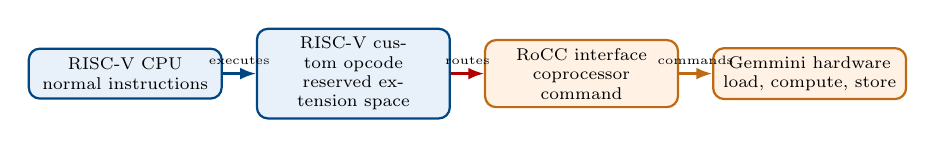
\begin{tikzpicture}[
    scale=0.88,
    every node/.style={transform shape},
    node distance=0.48cm,
    box/.style={rectangle,rounded corners,draw=ieeeblue,fill=ieeelight,thick,
      text width=2.55cm,minimum height=0.72cm,align=center,font=\scriptsize},
    hw/.style={rectangle,rounded corners,draw=stageorange,fill=orange!10,thick,
      text width=2.55cm,minimum height=0.72cm,align=center,font=\scriptsize},
    arrow/.style={-{Latex[length=2mm]},thick}
  ]
    \node[box] (cpu) {RISC-V CPU\\normal instructions};
    \node[box,right=of cpu] (custom) {RISC-V custom opcode\\reserved extension space};
    \node[hw,right=of custom] (rocc) {RoCC interface\\coprocessor command};
    \node[hw,right=of rocc] (gemmini) {Gemmini hardware\\load, compute, store};

    \draw[arrow,draw=ieeeblue] (cpu) -- node[above,font=\tiny]{executes} (custom);
    \draw[arrow,draw=red!70!black] (custom) -- node[above,font=\tiny]{routes} (rocc);
    \draw[arrow,draw=stageorange] (rocc) -- node[above,font=\tiny]{commands} (gemmini);
  \end{tikzpicture}

  \vspace{0.55em}
  \scriptsize
  \begin{tabularx}{\textwidth}{@{}lX@{}}
    \toprule
    Term & Meaning in this project \\
    \midrule
    \edgeword{Instruction} & A binary command decoded by the RISC-V core. Normal instructions do CPU work; custom instructions can command an attached accelerator. \\
    \edgeword{Custom instruction} & A RISC-V instruction using custom opcode space. The CPU recognizes that it belongs to a coprocessor path instead of a standard ALU/load/store path. \\
    \edgeword{RoCC} & Rocket Custom Coprocessor interface. It carries command fields from the CPU pipeline to Gemmini. \\
    \edgeword{Gemmini command} & The hardware meaning attached to a custom instruction, such as configure, move input, compute, or move output. \\
    \bottomrule
  \end{tabularx}

  \vspace{0.25em}
  \pathcode{src/Accelerators/Gemmini/Runtime/gemmini-hardware-abi/include/gemmini.h}
\end{frame}

% 40a
\begin{frame}{How a Gemmini Instruction Is Packed}
  \centering
  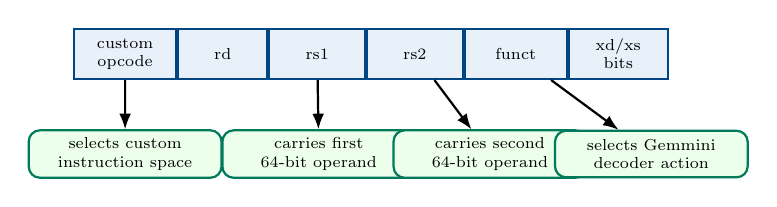
\begin{tikzpicture}[
    scale=0.82,
    every node/.style={transform shape},
    field/.style={rectangle,draw=ieeeblue,fill=ieeelight,thick,
      minimum height=0.78cm,align=center,font=\scriptsize},
    note/.style={rectangle,rounded corners,draw=stagegreen,fill=green!8,thick,
      text width=2.75cm,minimum height=0.72cm,align=center,font=\scriptsize},
    arrow/.style={-{Latex[length=2mm]},thick}
  ]
    \node[field,text width=1.35cm] (opcode) at (0,0) {custom\\opcode};
    \node[field,text width=1.15cm,right=0cm of opcode] (rd) {rd};
    \node[field,text width=1.25cm,right=0cm of rd] (rs1) {rs1};
    \node[field,text width=1.25cm,right=0cm of rs1] (rs2) {rs2};
    \node[field,text width=1.35cm,right=0cm of rs2] (funct) {funct};
    \node[field,text width=1.3cm,right=0cm of funct] (flags) {xd/xs\\bits};

    \node[note] (opn) at (0,-1.55) {selects custom\\instruction space};
    \node[note] (rs1n) at (3.0,-1.55) {carries first\\64-bit operand};
    \node[note] (rs2n) at (5.65,-1.55) {carries second\\64-bit operand};
    \node[note] (fn) at (8.15,-1.55) {selects Gemmini\\decoder action};

    \draw[arrow] (opcode) -- (opn);
    \draw[arrow] (rs1) -- (rs1n);
    \draw[arrow] (rs2) -- (rs2n);
    \draw[arrow] (funct) -- (fn);
  \end{tikzpicture}

  \vspace{0.6em}
  \scriptsize
  In \code{gemmini.h}, most commands use \code{ROCC\_INSTRUCTION\_RS1\_RS2(XCUSTOM\_ACC, rs1, rs2, funct)}.
  The C macro packs normal C values into registers, and the inline assembly emits a RISC-V custom instruction.

  \vspace{0.4em}
  \begin{block}{Why this matters}
    The same binary instruction is understood by three sides: C code knows the macro arguments, the RISC-V core knows how to issue the custom opcode, and Gemmini knows the \code{funct} command number.
  \end{block}
\end{frame}

% 40b
\begin{frame}[fragile]{Macro Path: C Helper to RoCC Instruction}
  \begin{lstlisting}
#define ROCC_INSTRUCTION_RS1_RS2(x, rs1, rs2, funct) \
  ROCC_INSTRUCTION_0_R_R(x, rs1, rs2, funct)

#define gemmini_extended_mvin(dram_addr, spad_addr, cols, rows) \
  ROCC_INSTRUCTION_RS1_RS2(XCUSTOM_ACC, dram_addr, \
    ((uint64_t)(rows) << (ADDR_LEN + 16)) | \
    ((uint64_t)(cols) << ADDR_LEN) | (spad_addr), k_MVIN)
  \end{lstlisting}
  \scriptsize
  \begin{tabularx}{\textwidth}{@{}lX@{}}
    \toprule
    Field & Explanation \\
    \midrule
    \edgeword{\code{XCUSTOM\_ACC}} & Selects the accelerator custom instruction slot used for Gemmini. \\
    \edgeword{\code{dram\_addr}} & First source register: host/DRAM address of the tensor tile. \\
    \edgeword{\code{rows, cols, spad\_addr}} & Packed into the second source register as tile shape plus scratchpad destination. \\
    \edgeword{\code{k\_MVIN}} & Function code telling Gemmini this command is a memory move into scratchpad. \\
    \bottomrule
  \end{tabularx}

  \vspace{0.2em}
  \pathcode{src/Accelerators/Gemmini/Runtime/gemmini-hardware-abi/include/gemmini.h}
\end{frame}

% 40c
\begin{frame}{Instruction Families Used by Gemmini}
  \scriptsize
  \begin{tabularx}{\textwidth}{@{}lXX@{}}
    \toprule
    Family & Example function codes & Purpose \\
    \midrule
    \edgeword{Configure} &
      \code{k\_CONFIG}, \code{CONFIG\_EX}, \code{CONFIG\_LD}, \code{CONFIG\_ST} &
      Program execution mode, dataflow, activation, strides, load scaling, and store behavior. \\
    \edgeword{Move in} &
      \code{k\_MVIN}, \code{k\_MVIN2}, \code{k\_MVIN3} &
      Move input, weights, or bias tiles from DRAM into Gemmini scratchpad or accumulator memory. \\
    \edgeword{Compute} &
      \code{k\_PRELOAD}, \code{k\_COMPUTE\_PRELOADED}, \code{k\_COMPUTE\_ACCUMULATE} &
      Feed matrix tiles into the systolic array and accumulate partial results. \\
    \edgeword{Move out} &
      \code{k\_MVOUT}, \code{k\_MVOUT\_SPAD} &
      Copy completed output tiles from Gemmini memory back to DRAM. \\
    \edgeword{Hardware loops} &
      \code{k\_LOOP\_WS}, \code{k\_LOOP\_CONV\_WS} &
      Let Gemmini run larger matmul/conv loops after receiving packed bounds, addresses, and strides. \\
    \bottomrule
  \end{tabularx}

  \vspace{0.4em}
  \begin{block}{Simple rule}
    \code{k\_*} values are not CPU functions. They are command IDs decoded by Gemmini hardware after the RoCC instruction reaches the accelerator.
  \end{block}
\end{frame}

% 40d
\begin{frame}{How Conv Becomes Several Custom Instructions}
  \centering
  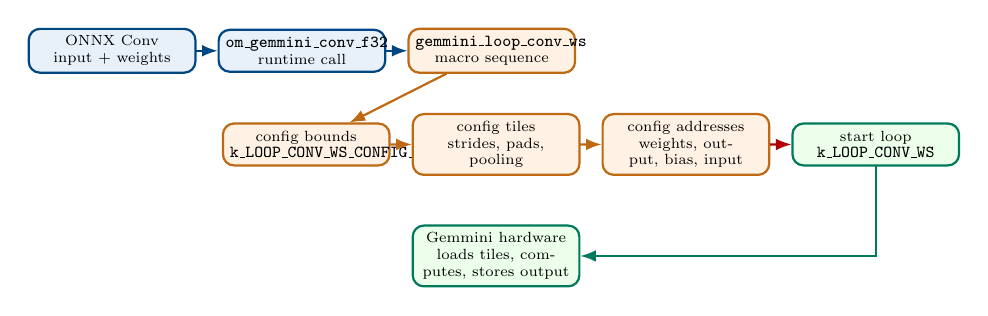
\begin{tikzpicture}[
    scale=0.76,
    every node/.style={transform shape},
    node distance=0.36cm,
    sw/.style={rectangle,rounded corners,draw=ieeeblue,fill=ieeelight,thick,
      text width=2.55cm,minimum height=0.70cm,align=center,font=\scriptsize},
    cmd/.style={rectangle,rounded corners,draw=stageorange,fill=orange!10,thick,
      text width=2.55cm,minimum height=0.70cm,align=center,font=\scriptsize},
    hw/.style={rectangle,rounded corners,draw=stagegreen,fill=green!8,thick,
      text width=2.55cm,minimum height=0.70cm,align=center,font=\scriptsize},
    arrow/.style={-{Latex[length=2mm]},thick}
  ]
    \node[sw] (onnx) {ONNX Conv\\input + weights};
    \node[sw,right=of onnx] (rt) {\code{om\_gemmini\_conv\_f32}\\runtime call};
    \node[cmd,right=of rt] (loop) {\code{gemmini\_loop\_conv\_ws}\\macro sequence};

    \node[cmd,below=0.82cm of loop,xshift=-3.1cm] (c1) {config bounds\\\code{k\_LOOP\_CONV\_WS\_CONFIG\_1}};
    \node[cmd,right=of c1] (c2) {config tiles\\strides, pads, pooling};
    \node[cmd,right=of c2] (c3) {config addresses\\weights, output, bias, input};
    \node[hw,right=of c3] (go) {start loop\\\code{k\_LOOP\_CONV\_WS}};

    \node[hw,below=0.82cm of c2] (gem) {Gemmini hardware\\loads tiles, computes, stores output};

    \draw[arrow,draw=ieeeblue] (onnx) -- (rt);
    \draw[arrow,draw=ieeeblue] (rt) -- (loop);
    \draw[arrow,draw=stageorange] (loop) -- (c1);
    \draw[arrow,draw=stageorange] (c1) -- (c2);
    \draw[arrow,draw=stageorange] (c2) -- (c3);
    \draw[arrow,draw=red!70!black] (c3) -- (go);
    \draw[arrow,draw=stagegreen] (go) |- (gem);
  \end{tikzpicture}

  \vspace{0.45em}
  \scriptsize
  One ONNX Conv is larger than one hardware instruction. The runtime expands it into a command sequence that gives Gemmini dimensions, addresses, padding, strides, activation, and launch information.
\end{frame}

% 40e
\begin{frame}[fragile]{Conv Loop Macro Sends Configuration Commands}
  \begin{lstlisting}
#define gemmini_loop_conv_ws(..., weights, output, bias, input, ...) \
  { \
    ROCC_INSTRUCTION_RS1_RS2(XCUSTOM_ACC, packed_dims_1, packed_dims_2, \
      k_LOOP_CONV_WS_CONFIG_1) \
    ROCC_INSTRUCTION_RS1_RS2(XCUSTOM_ACC, packed_tile_1, packed_tile_2, \
      k_LOOP_CONV_WS_CONFIG_2) \
    ROCC_INSTRUCTION_RS1_RS2(XCUSTOM_ACC, weights, output, \
      k_LOOP_CONV_WS_CONFIG_5) \
    ROCC_INSTRUCTION_RS1_RS2(XCUSTOM_ACC, bias, input, \
      k_LOOP_CONV_WS_CONFIG_6) \
    ROCC_INSTRUCTION_RS1_RS2(XCUSTOM_ACC, packed_flags_1, packed_flags_2, \
      k_LOOP_CONV_WS) \
  }
  \end{lstlisting}
  \scriptsize
  The real macro has many parameters because convolution needs many facts:
  tensor sizes, kernel size, padding, stride, pooling, weight address, input address, bias address, output address, activation, and layout flags.

  \vspace{0.25em}
  \pathcode{src/Accelerators/Gemmini/Runtime/gemmini-hardware-abi/include/gemmini.h}
\end{frame}

% 40f
\begin{frame}{How to Read \code{.insn} in Disassembly}
  \scriptsize
  \begin{tabularx}{\textwidth}{@{}lX@{}}
    \toprule
    Disassembly part & Meaning \\
    \midrule
    \edgeword{Address} & The left address, for example \code{181be}, is where this instruction lives in the linked RV64 executable. \\
    \edgeword{Hex word} & The middle value, for example \code{00e8b07b}, is the raw 32-bit instruction encoding. \\
    \edgeword{\code{.insn}} & The disassembler does not know a nice Gemmini mnemonic, so it prints the generic custom-instruction form. \\
    \edgeword{Runtime location} & These instructions usually appear inside linked Gemmini runtime/helper code, not directly beside the original ONNX node text. \\
    \edgeword{Proof of hardware path} & Seeing \code{.insn} confirms the binary contains RoCC/Gemmini commands, not only CPU fallback code. \\
    \bottomrule
  \end{tabularx}

  \vspace{0.45em}
  \begin{block}{Important}
    \code{.insn} is not an error. It is the assembler/disassembler's generic way to represent an instruction whose exact accelerator meaning is defined by the Gemmini ABI and hardware decoder.
  \end{block}
\end{frame}

% 40g
\begin{frame}{Break Down \code{00e8b07b}}
  \scriptsize
  \begin{block}{Main idea}
    This \code{.insn} line is not a mistake and not a generic placeholder. It is a custom RISC-V instruction that the RISC-V core forwards through RoCC to the Gemmini accelerator.
  \end{block}

  \vspace{0.25em}
  \begin{tabularx}{\textwidth}{@{}lX@{}}
    \toprule
    Field & What it means \\
    \midrule
    \edgeword{\code{0x7b} opcode} &
      The low 7 bits are \code{0x7b}, which is RISC-V \code{custom-3}. RISC-V reserves custom opcode spaces such as \code{0x0b} custom-0, \code{0x2b} custom-1, \code{0x5b} custom-2, and \code{0x7b} custom-3 so extensions do not collide with standard instructions. \\
    \edgeword{\code{funct7}} &
      The high command field selects the Gemmini decoder action. In Gemmini, these values distinguish configuration, data movement, compute, loop setup, and other accelerator commands. \\
    \edgeword{Register fields} &
      The middle bits encode \code{rd}, \code{rs1}, and \code{rs2}. The registers carry values such as DRAM addresses, scratchpad addresses, packed tile sizes, strides, or command flags. \\
    \edgeword{Execution} &
      The CPU does not treat this like a normal ALU instruction. It issues a RoCC command packet containing the instruction and the selected register values. Gemmini decodes that packet and performs the low-level accelerator operation. \\
    \bottomrule
  \end{tabularx}
\end{frame}

% 40h
\begin{frame}{How \code{00e8b07b} Reaches Gemmini}
  \centering
  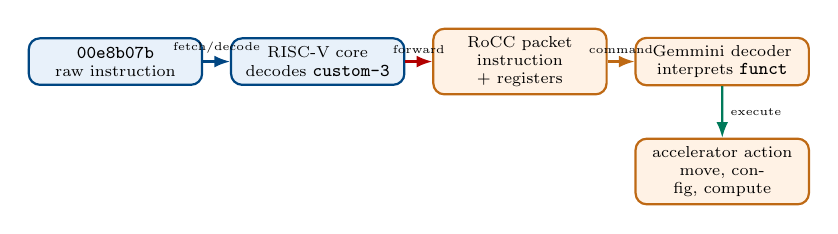
\begin{tikzpicture}[
    scale=0.82,
    every node/.style={transform shape},
    node distance=0.42cm,
    box/.style={rectangle,rounded corners,draw=ieeeblue,fill=ieeelight,thick,
      text width=2.45cm,minimum height=0.72cm,align=center,font=\scriptsize},
    hw/.style={rectangle,rounded corners,draw=stageorange,fill=orange!10,thick,
      text width=2.45cm,minimum height=0.72cm,align=center,font=\scriptsize},
    arrow/.style={-{Latex[length=2mm]},thick}
  ]
    \node[box] (dis) {\code{00e8b07b}\\raw instruction};
    \node[box,right=of dis] (decode) {RISC-V core\\decodes \code{custom-3}};
    \node[hw,right=of decode] (packet) {RoCC packet\\instruction + registers};
    \node[hw,right=of packet] (gem) {Gemmini decoder\\interprets \code{funct}};
    \node[hw,below=0.8cm of gem] (work) {accelerator action\\move, config, compute};

    \draw[arrow,draw=ieeeblue] (dis) -- node[above,font=\tiny]{fetch/decode} (decode);
    \draw[arrow,draw=red!70!black] (decode) -- node[above,font=\tiny]{forward} (packet);
    \draw[arrow,draw=stageorange] (packet) -- node[above,font=\tiny]{command} (gem);
    \draw[arrow,draw=stagegreen] (gem) -- node[right,font=\tiny]{execute} (work);
  \end{tikzpicture}

  \vspace{0.55em}
  \scriptsize
  The line is machine code for telling Gemmini to perform one low-level hardware operation. A complete convolution or matrix multiplication is built from several such commands, plus normal RISC-V instructions and runtime control code.

  \vspace{0.25em}
  \pathcode{src/Accelerators/Gemmini/Runtime/gemmini-hardware-abi/rocc-software/src/xcustom.h}
\end{frame}

% 40i
\begin{frame}[fragile]{Example: Gemmini Custom Instructions}
  \begin{lstlisting}
181be: 00e8b07b  .insn 4, 0x00e8b07b
18234: 04e5b07b  .insn 4, 0x04e5b07b
18262: 00f7307b  .insn 4, 0x00f7307b
182cc: 05e8307b  .insn 4, 0x05e8307b
182fc: 04f8307b  .insn 4, 0x04f8307b
  \end{lstlisting}
  \begin{itemize}
    \item These lines appear in \code{resnet18\_rv64.disasm}.
    \item The generic disassembler prints raw custom RISC-V encodings as \code{.insn}.
    \item They correspond to Gemmini RoCC operations emitted by the ABI/runtime path.
  \end{itemize}
\end{frame}

% 40b
\begin{frame}{How Generated Code Transfers Tensors to Runtime}
  \centering
  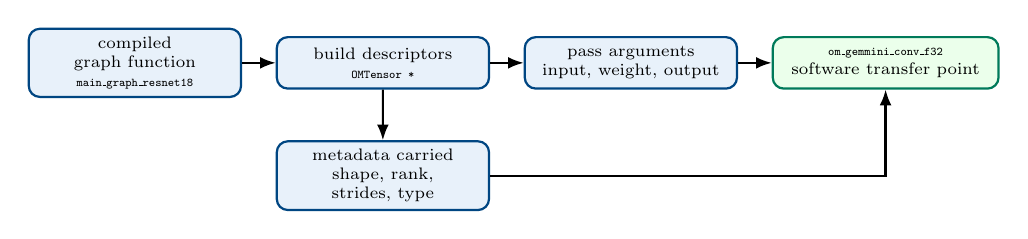
\begin{tikzpicture}[
    scale=0.86,
    every node/.style={transform shape},
    node distance=0.5cm,
    box/.style={rectangle,rounded corners,draw=ieeeblue,fill=ieeelight,thick,
      text width=2.9cm,minimum height=0.76cm,align=center,font=\scriptsize},
    rt/.style={rectangle,rounded corners,draw=stagegreen,fill=green!8,thick,
      text width=3.1cm,minimum height=0.76cm,align=center,font=\scriptsize},
    arrow/.style={-{Latex[length=2mm]},thick}
  ]
    \node[box] (graph) {compiled graph function\\\tinycode{main\_graph\_resnet18}};
    \node[box,right=of graph] (desc) {build descriptors\\\tinycode{OMTensor *}};
    \node[box,right=of desc] (args) {pass arguments\\input, weight, output};
    \node[rt,right=of args] (runtime) {\tinycode{om\_gemmini\_conv\_f32}\\software transfer point};
    \node[box,below=0.75cm of desc] (meta) {metadata carried\\shape, rank, strides, type};

    \draw[arrow] (graph) -- (desc);
    \draw[arrow] (desc) -- (args);
    \draw[arrow] (args) -- (runtime);
    \draw[arrow] (desc) -- (meta);
    \draw[arrow] (meta) -| (runtime);
  \end{tikzpicture}

  \vspace{0.45em}
  \begin{block}{Meaning}
    The generated code does not directly program Gemmini. It hands tensor descriptors to a runtime function with a stable C ABI.
  \end{block}
\end{frame}

% 40c
\begin{frame}{How Runtime Transfers Data to Gemmini Hardware}
  \centering
  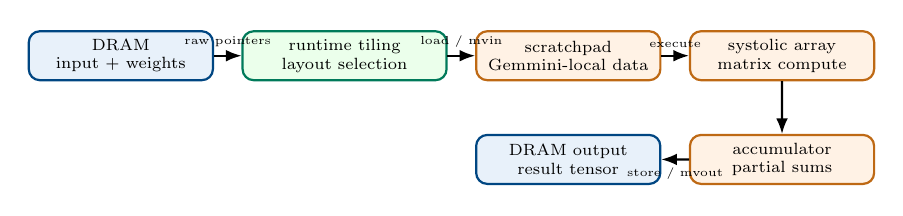
\begin{tikzpicture}[
    scale=0.84,
    every node/.style={transform shape},
    node distance=0.42cm,
    mem/.style={rectangle,rounded corners,draw=ieeeblue,fill=ieeelight,thick,
      text width=2.55cm,minimum height=0.74cm,align=center,font=\scriptsize},
    rt/.style={rectangle,rounded corners,draw=stagegreen,fill=green!8,thick,
      text width=2.85cm,minimum height=0.74cm,align=center,font=\scriptsize},
    hw/.style={rectangle,rounded corners,draw=stageorange,fill=orange!10,thick,
      text width=2.55cm,minimum height=0.74cm,align=center,font=\scriptsize},
    arrow/.style={-{Latex[length=2mm]},thick}
  ]
    \node[mem] (dram) {DRAM\\input + weights};
    \node[rt,right=of dram] (tile) {runtime tiling\\layout selection};
    \node[hw,right=of tile] (spad) {scratchpad\\Gemmini-local data};
    \node[hw,right=of spad] (compute) {systolic array\\matrix compute};
    \node[hw,below=0.8cm of compute] (acc) {accumulator\\partial sums};
    \node[mem,left=of acc] (out) {DRAM output\\result tensor};

    \draw[arrow] (dram) -- node[above,font=\tiny] {raw pointers} (tile);
    \draw[arrow] (tile) -- node[above,font=\tiny] {load / mvin} (spad);
    \draw[arrow] (spad) -- node[above,font=\tiny] {execute} (compute);
    \draw[arrow] (compute) -- (acc);
    \draw[arrow] (acc) -- node[below,font=\tiny] {store / mvout} (out);
  \end{tikzpicture}

  \vspace{0.4em}
  \begin{block}{Meaning}
    Runtime turns model-level tensors into hardware-level transfers: DRAM to scratchpad, scratchpad to compute, accumulator back to DRAM.
  \end{block}
\end{frame}

% 40d
\begin{frame}{Why Transfer Cost Matters}
  \begin{itemize}
    \item Gemmini acceleration is only useful if transfer overhead is controlled.
    \item Tiling decides how much data is moved at once.
    \item Scratchpad reuse reduces repeated DRAM traffic.
    \item Weight constants live in ELF \code{.rodata}; at runtime they are read through pointers and moved into Gemmini-local storage.
  \end{itemize}
\end{frame}

% 41
\begin{frame}{How Conv Moves from ONNX to Binary}
  \begin{enumerate}
    \item ONNX model contains a Conv node and constant weight tensors.
    \item ONNX-MLIR imports the graph into ONNX dialect MLIR.
    \item Gemmini conversion chooses supported Conv operations.
    \item Lowering produces runtime calls such as \code{om\_gemmini\_conv\_f32}.
    \item LLVM produces RV64 object code.
    \item Linker combines model object, Gemmini runtime archive, C runtime archive, and runner.
    \item Disassembly shows calls and raw Gemmini custom instructions.
  \end{enumerate}
\end{frame}

% 42
\begin{frame}{Why Runtime Calls Appear Before Raw Instructions}
  \begin{itemize}
    \item A model-level Conv involves tensor descriptors, shapes, strides, padding, allocation, and cleanup.
    \item It is more maintainable to call a runtime wrapper for complex setup.
    \item The runtime can implement tiling, packing, quantization, and Gemmini kernel calls.
    \item The low-level Gemmini kernel eventually emits custom instructions through the ABI macros.
  \end{itemize}
\end{frame}

% 43
\sectiondivider{Validation and Takeaways}{Use the artifact chain to debug, validate, and explain the pipeline.}

\begin{frame}{Troubleshooting Map: Where Did Conv Go?}
  \centering
  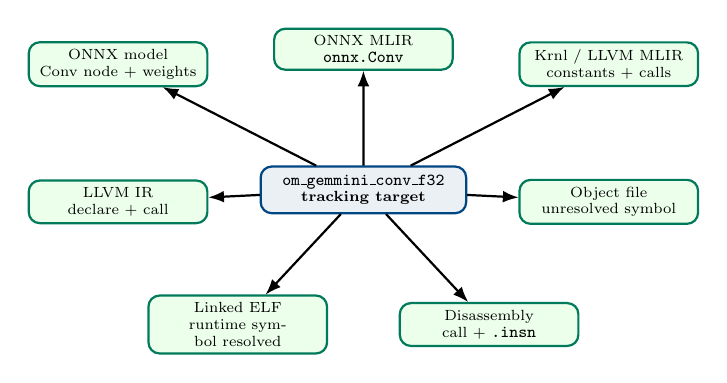
\begin{tikzpicture}[
    scale=0.76,
    every node/.style={transform shape},
    center/.style={rectangle,rounded corners,draw=ieeeblue,fill=ieeeblue!8,thick,
      text width=3.2cm,minimum height=0.78cm,align=center,font=\scriptsize\bfseries},
    check/.style={rectangle,rounded corners,draw=stagegreen,fill=green!8,thick,
      text width=2.75cm,minimum height=0.68cm,align=center,font=\scriptsize},
    warn/.style={rectangle,rounded corners,draw=red!70!black,fill=red!8,thick,
      text width=2.75cm,minimum height=0.68cm,align=center,font=\scriptsize},
    arrow/.style={-{Latex[length=2mm]},thick}
  ]
    \node[center] (conv) at (0,0) {\code{om\_gemmini\_conv\_f32}\\tracking target};
    \node[check] (onnx) at (-4.1,2.1) {ONNX model\\Conv node + weights};
    \node[check] (mlir) at (0,2.35) {ONNX MLIR\\\code{onnx.Conv}};
    \node[check] (krnl) at (4.1,2.1) {Krnl / LLVM MLIR\\constants + calls};
    \node[check] (ll) at (-4.1,-0.2) {LLVM IR\\declare + call};
    \node[check] (obj) at (4.1,-0.2) {Object file\\unresolved symbol};
    \node[check] (elf) at (-2.1,-2.25) {Linked ELF\\runtime symbol resolved};
    \node[check] (dis) at (2.1,-2.25) {Disassembly\\call + \code{.insn}};

    \draw[arrow] (conv) -- (onnx);
    \draw[arrow] (conv) -- (mlir);
    \draw[arrow] (conv) -- (krnl);
    \draw[arrow] (conv) -- (ll);
    \draw[arrow] (conv) -- (obj);
    \draw[arrow] (conv) -- (elf);
    \draw[arrow] (conv) -- (dis);
  \end{tikzpicture}
  \vspace{0.35em}
  \begin{block}{Debug rule}
    If Conv disappears, check the first missing artifact: unsupported ONNX pattern, missing runtime declaration, link failure, or ABI/custom-instruction path.
  \end{block}
\end{frame}

\begin{frame}{Validation Checklist}
  \begin{itemize}
    \item Check the MLIR files after each important pass.
    \item Confirm runtime calls in \code{resnet18.ll}.
    \item Confirm the final ELF is RV64 and statically linked as expected.
    \item Confirm disassembly includes \code{om\_gemmini\_conv\_f32} calls.
    \item Confirm Gemmini custom instructions appear as \code{.insn} in disassembly.
    \item Compare Spike timing JSON outputs for Gemmini vs non-Gemmini.
  \end{itemize}
\end{frame}

% 45
\begin{frame}{Key Takeaways}
  \scriptsize
  \begin{tabularx}{\textwidth}{@{}lX@{}}
    \toprule
    Takeaway & What to remember \\
    \midrule
    \edgeword{Compiler lowers meaning} &
      ONNX starts as graph semantics and becomes Gemmini/LLVM/RV64 execution details. \\
    \edgeword{Runtime bridges tensors} &
      Generated code calls stable functions that understand \code{OMTensor} and \code{OMTensorList}. \\
    \edgeword{ABI protects binary agreement} &
      C calls and Gemmini hardware commands work only when caller and callee agree. \\
    \edgeword{GemminiLow exposes hardware} &
      Config, load, execute, and store become visible before final LLVM/RV64 lowering. \\
    \edgeword{Artifacts prove the path} &
      Follow Conv through ONNX, MLIR, LLVM IR, object, ELF, and disassembly. \\
    \bottomrule
  \end{tabularx}
\end{frame}

\begin{frame}{What This Pipeline Achieves}
  \begin{itemize}
    \item ONNX-MLIR supplies the multi-level compiler infrastructure.
    \item Gemmini adds accelerator-specific dialects, conversion passes, runtime code, and ABI integration.
    \item Gemmini is the high-level accelerator dialect; GemminiLow is the hardware-oriented dialect.
    \item The ResNet-18 example demonstrates the full path from model artifacts to RV64 ELF and disassembly.
  \end{itemize}
  \vfill
  \begin{center}
    \textbf{Project: Gemmini Pipeline in ONNX-MLIR}\\
    \textbf{Company: Siliconesignal Technologies}\\
    July 15, 2026
  \end{center}
\end{frame}

\end{document}
